%% ---------------------------------------------------------------------------
%% Main file -- Accuracy analysis of Kirchhoff plate theory
%% Typeset with the Elsevier CAS single-column class (cas-sc.cls).
%% ---------------------------------------------------------------------------
%% Document class
%\documentclass[a4paper,fleqn,longmktitle]{cas-sc}
\documentclass[a4paper,fleqn]{cas-sc}

%% ---------------------------------------------------------------------------
%% Bibliography: numeric citations, sorted and compressed (e.g. [1-7])
%% ---------------------------------------------------------------------------
%\usepackage[numbers]{natbib}
\usepackage[numbers,sort&compress]{natbib}

%% ---------------------------------------------------------------------------
%% Mathematics
%% ---------------------------------------------------------------------------
\usepackage{amsmath}
\usepackage{amssymb}
\usepackage{amsfonts}
\usepackage{bm}

%% ---------------------------------------------------------------------------
%% Graphics, tables and lists
%% ---------------------------------------------------------------------------
\usepackage{graphicx}
\usepackage{booktabs}
\usepackage{array}
\usepackage{multirow}

%% ---------------------------------------------------------------------------
%% Author macros (as in the CAS sample file)
%% ---------------------------------------------------------------------------
\def\tsc#1{\csdef{#1}{\textsc{\lowercase{#1}}\xspace}}
\tsc{WGM}
\tsc{QE}
\tsc{EP}
\tsc{PMS}
\tsc{BEC}
\tsc{DE}

%% Frequently used notation shortcuts
\newcommand{\dd}{\mathrm{d}}
\newcommand{\A}{\mathrm{A}}
\newcommand{\F}{\mathrm{F}}
\newcommand{\B}{\mathrm{B}}
\newcommand{\bA}{\mathbf{A}}
\newcommand{\bB}{\mathbf{B}}
\newcommand{\bF}{\mathbf{F}}
\newcommand{\bD}{\mathbf{D}}
\newcommand{\bN}{\mathbb{N}}
\newcommand{\bP}{\mathbb{P}}
\newcommand{\sk}{\operatorname{span}}
\newcommand{\supp}{\operatorname{supp}}
\newcommand{\bt}[1]{\tilde{#1}}

\begin{document}
\let\WriteBookmarks\relax
\def\floatpagepagefraction{1}
\def\textpagefraction{.001}
\shorttitle{Accuracy analysis of Kirchhoff plate theory}
\shortauthors{H.~Du et~al.}

%% ---------------------------------------------------------------------------
%% Front matter
%% ---------------------------------------------------------------------------
\title[mode = title]{Accuracy analysis of Kirchhoff plate theory}

%% NOTE: author names, affiliations and funding information were not available
%% in the source Word file.  Please complete the fields below.
\author[1]{First A. Author}[type=editor,
                        auid=000,bioid=1,
                        role=Researcher,
                        orcid=0000-0000-0000-0000]
\cormark[1]
\ead{author@example.edu}

\affiliation[1]{organization={Department of Engineering Mechanics},
                city={City},
                postcode={000000},
                country={China}}

\cortext[cor1]{Corresponding author}

%% ---------------------------------------------------------------------------
%% Body -- one file per section
%% ---------------------------------------------------------------------------
%% ---------------------------------------------------------------------------
%% Abstract and keywords
%% ---------------------------------------------------------------------------
\begin{abstract}
It is well known that numerical integration plays crucial roles in Galerkin meshfree methods for elasticity problems,
since inappropriate integration methods would lead to the loss of orthogonality condition, which is a basic part for evaluating the convergence performance.
As an extension of the works for second order problems, explicit estimates of $L_2$, $H_1$ and $H_2$ errors for Galerkin meshfree formulation to Kirchhoff plate (fourth order problem) was presented in this work.
Specifically, accounting for the effect of numerical integration, the $H_2$ error bound for orthogonally condition of Galerkin meshfree formulation was investigated, then it was regarded as a basic component to measure $H_2$ error of Galerkin meshfree methods.
Subsequently, with the help of closed graph theorem and Lagrange interpolation, the $L_2$ and $H_1$ error formulas of Galerkin meshfree methods was established and then divided into two components, which are respectively related to the standard error and integration error.
After that, the standard error was separately investigated with considering different orders of Lagrange interpolation for different orders of meshfree approximation.
It turns out that when the consistency of integral schemes satisfies the same order of meshfree approximation ($p=q$), an optimal convergence performance of meshfree methods to Kirchhoff plate will be achieved.
Furthermore, only when the order of meshfree approximation is greater than two ($p>2$) and the integral schemes possess the above property about consistency ($p=q$), a $(p+1)$th order of convergence rate can be realized.
Numerical examples well validate the proposed theory.
\end{abstract}

\begin{keywords}
Galerkin meshfree method \sep Kirchhoff plate \sep numerical integration \sep integration constraint \sep error estimate
\end{keywords}

\maketitle

%% ---------------------------------------------------------------------------
%% 1. Introduction
%% ---------------------------------------------------------------------------
\section{Introduction}

As a node-based numerical method, the meshfree methods enable an efficient and straightforward way to construct arbitrary order smooth shape function \cite{ref1,ref2,ref3,ref4,ref5,ref6,ref7} and execute post process without full-connected elements like in finite element methods \cite{ref8}.
In weak form based meshfree methods, Galerkin meshfree methods invoke Galerkin weak form of equilibrium equations thus lower the continuity requirements of approximation, which greatly improves the stability and accuracy \cite{ref1,ref5}.
Consequently, Galerkin meshfree methods have attracted lots of attention among scholars and developed into various kinds of approaches, such as Element-free Galerkin method \cite{ref9,ref10}, reproducing kernel particle method \cite{ref11}, max-entropy meshfree method \cite{ref12}, smoothed particle Galerkin method \cite{ref13}, among others \cite{ref14,ref20}.

Additionally, due to the arbitrary order smooth approximants, it is a desirable way to apply the Galerkin meshfree methods on the higher order problems like Kirchhoff--Love plate theory, which requires at least $C^1$ continuity of shape function for Galerkin weak form.
Specifically, Krysl et al. \cite{ref21} adopted element-free Galerkin method to analyze the thin plates.
Subsequently, Liu et al. \cite{ref22,ref23} theoretically investigate the performance of element-free Galerkin method in static and dynamic analysis of thin plates.
Petrov--Galerkin meshfree method is applied in static and dynamic analysis by Gu and Liu \cite{ref24}.
By combining triangular integration cell with RK approximation, Simkins et al. \cite{ref25} proposed reproducing kernel element method and assessment its performance in solving Kirchhoff--Love plate problems.
With the expectation of improving efficiency and conveniently imposing rotation boundary condition, Wang and Chen \cite{ref26} introduced rotation variable into reproducing kernel approximation, and presented a Hermite reproducing kernel approximation for thin plates analysis.
By introducing reproducing polynomial particle approximation, Oh et al. \cite{ref27} proposed a meshfree particle method for thin plates, which has high order reproducing property and the Kronecker delta property.
Based on linear basis function, Deng et al. \cite{ref28} proposed a gradient smoothing Galerkin meshfree method to eliminate the necessity of $C^1$ continuous approximation.

It should be noted that meshfree shape function usually possess rational nature, which brings severe difficulty towards accurate numerical integration \cite{ref29,ref30}.
The integration constraints which has been numerically proved play a crucial role in convergence performance of Galerkin meshfree methods \cite{ref31,ref32,ref33,ref34,ref35}, was first proposed and validated by Chen et al \cite{ref31,ref32}.
In order to satisfy the integration constraints or realize integration consistency, lots of approaches have been presented and applied in many problems \cite{ref33,ref34,ref35,ref36,ref37,ref38,ref39,ref40,ref41,ref42,ref43,ref44}.
More specifically, Chen et al. \cite{ref31,ref32} replaced the derivate of shape function by strain smoothing technology such that the linear integration constraints have been satisfied.
By solving sets of equations generated by quadratic integration constraints, Duan et al. \cite{ref35,ref40} proposed quadratically consistent meshfree integration method, which are further developed and applied in strain gradient elasticity.
Wang et al. \cite{ref42} extended SCNI into quadratic meshfree formulation and proposed sub-domain stabilized conforming integration scheme in order to meet the quadratic integration constraints.
Based upon reproducing kernel approximation, Wang and Wu \cite{ref43} presented an inherently consistent reproducing kernel gradient smoothing integration algorithm (RKGSI), which automatically meet arbitrary order of basis function.
Thereafter, Du et al. \cite{ref45} presented a unified reproducing kernel gradient smoothing approach as extension and application of RKGSI in higher order problems.

Regarding to error estimates of Galerkin meshfree methods, Liu et al. \cite{ref46} measured the convergence rate of MLS reproducing kernel methods (MLSRKPM) by a dilation parameter of window function.
Salehi and Dehghan \cite{ref47} conducted the error estimated for a class of time-dependent partial differential equations studied by the proposed MLS radial reproducing polynomial meshless method (MLSRRPM).
Han and Meng \cite{ref48} introduced a theoretical analysis of the reproducing kernel particle method (RKPM) by interpolation error estimates.
Osorio and French \cite{ref49} theoretically validated the advantages of proposed stabilized diffuse Galerkin method (SDGM) by providing error estimates.
Among them, the importance of integration consistency has not been theoretically proved although lots of numerical experiments have well shown the desirable convergence performance of methods with integration consistency.

Recently, Wu and Wang \cite{ref50} took the effect of numerical integration into consideration, providing a valuable error analysis of Galerkin meshfree methods for second order problems like potential problems and elasticity problems.
As an extension of the previous work, we focus on the fourth order Kirchhoff--Love plate problems, investigating the crucial role of integration constraints and meshfree approximations.
Firstly, we estimate the convergence rate of $H_2$ error of Galerkin meshfree methods for thin plates, which is strongly related to the order of integration consistency and meshfree approximation.
Then, with the help of the closed graph theorem \cite{ref51} and Lagrange interpolants, we further investigate the $L_2$ and $H_1$ error estimates by dividing them into two parts, which is related to the standard error of meshfree approximation and error of orthogonality, respectively.
Subsequently, in light of constrains on the order selection of Lagrange interpolation from meshfree approximation, the error estimate for first part is further divided into two cases, the order of meshfree approximation is greater than or equal to three ($p\ge3$), and equal to two ($p=2$).
It turns out that, only when the order of meshfree approximation satisfy the minimum requirement ($p\ge3$) and integration schemes possess corresponding order of integration constraints, can the Galerkin meshfree methods achieve optimal convergence performance.
The numerical experiments well demonstrate the presented theoretical results.

The remainder of this paper is organized as follows.
Section \ref{sec:formulation} introduces the discrete Galerkin meshfree formulation for Kirchhoff--Love plate, and the reproducing kernel gradient smoothing integration scheme is described.
Section \ref{sec:error} is devoted to the error estimates of the Galerkin meshfree formulation in $H_2$, $H_1$ and $L_2$ norms.
Numerical examples are examined in Section \ref{sec:numerical} and the conclusions are drawn in Section \ref{sec:conclusion}.

%% ---------------------------------------------------------------------------
%% 2. Discrete Galerkin meshfree formulation for Kirchhoff--Love plate
%% ---------------------------------------------------------------------------
\section{Discrete Galerkin meshfree formulation for Kirchhoff--Love plate}\label{sec:formulation}

\subsection{Galerkin weak form of Kirchhoff--Love plate}

In accordance with the Kirchhoff--Love plate theory, the equilibrium equation and boundary conditions of an elastic body $\Omega$ with boundary $\Gamma$ can be stated as follows:
\begin{equation}\label{eq:1}
\begin{cases}
-M_{ij,ij}=q & \text{in }\Omega\\[2pt]
w=\bar{w} & \text{on }\Gamma^{w}\\[2pt]
w_{,n_i}=\bar{\theta}_{n} & \text{on }\Gamma^{\theta}\\[2pt]
M_{ij,j}n_i+M_{ns,s}=\bar{V} & \text{on }\Gamma^{V}\\[2pt]
M_{ij}n_in_j=\bar{M}_{n} & \text{on }\Gamma^{M}\\[2pt]
M_{ns}=\bar{F}_{c} & \text{at }\Gamma^{c}
\end{cases}
\end{equation}
where $M_{ij}=-C_{ijkl}w_{,kl}$ and $q$ represent the moment and loading along the plate.
$\Gamma^{w}$ and $\Gamma^{\theta}$ denote the displacement and slope boundaries, $\bar{w}$ and $\bar{\theta}_{n}$ are the corresponding given values.
$\bm{n}=\{n_i\}$ and $\bm{s}=\{s_i\}$ represent the boundary outward normal and tangent.
$\bar{V}$, $\bar{M}_{n}$ and $\bar{M}_{ns}=M_{jk}s_jn_k$ denote the equivalent shear force, moment and torque on the natural boundaries $\Gamma^{V}$ and $\Gamma^{M}$, respectively.
In addition, $\bar{F}_{c}$ is the concentrated force at the corners of boundary curve $\Gamma^{c}$.

The weak form of Kirchhoff--Love plate can be established as follows:
\begin{equation}\label{eq:2}
\int_{\Omega}\delta w\left(M_{ij,ij}+q\right)\dd\Omega=0
\end{equation}
where $\delta w$ denotes an arbitrary test function or virtual displacement.
By invoking the procedure of integration by parts, Eq. \eqref{eq:2} becomes:
\begin{equation}\label{eq:3}
\int_{\Omega}\delta w_{,ij}M_{ij}\dd\Omega
=-\int_{\Gamma}\delta wM_{ij,j}n_i\dd\Gamma
-\int_{\Omega}\delta wq\dd\Omega
+\int_{\Gamma}\delta w_{,j}M_{ij}n_i\dd\Gamma
\end{equation}
To achieve independent and meaningful boundary conditions, the last term in Eq. \eqref{eq:3} is further divided into two parts:
\begin{equation}\label{eq:4}
\begin{aligned}
\int_{\Gamma}\delta w_{,i}M_{ij}n_j\dd\Gamma
&=\int_{\Gamma}\delta w_{,i}\underbrace{\delta_{ij}}_{=\,n_in_j+s_is_j}M_{jk}n_k\dd\Gamma\\[2pt]
&=\int_{\Gamma}\delta w_{,i}\underbrace{n_i}_{=\,\delta w_{,n}}n_jM_{jk}n_k\dd\Gamma
+\int_{\Gamma}\delta w_{,i}\underbrace{s_i}_{=\,\delta w_{,s}}s_jM_{jk}n_k\dd\Gamma\\[2pt]
&=\int_{\Gamma}\delta w_{,n}\bar{M}_{n}\dd\Gamma
-\int_{\Gamma}\delta w\left(s_jM_{jk}n_k\right)_{,s}\dd\Gamma
+\left[\delta ws_jM_{jk}n_k\right]_{\Gamma}\\[2pt]
&=\int_{\Gamma}\delta w_{,n}\bar{M}_{n}\dd\Gamma
-\int_{\Gamma}\delta wM_{ns,s}\dd\Gamma
+\left[\delta wM_{ns}\right]_{\Gamma}
\end{aligned}
\end{equation}
Meanwhile, with the smooth boundary surface assumption, the second term in the right of Eq. \eqref{eq:4} can be eliminated:
\begin{equation}\label{eq:5}
\left[\delta wM_{ns}\right]_{\Gamma}
=\sum_{m=1}^{n_{c}}\left\{\left[\delta wM_{ns}\right](c_{m+1})-\left[\delta wM_{ns}\right](c_{m})\right\}=0
\end{equation}
where $n_{c}$ represents the number of convex points in closed boundary curve, where the corner index $c_{m+1}$ is identified with corner index $c_{m}$.

In order to obtain the general form without assumption, here we still adopt Eq. \eqref{eq:3} to further deduce the weak form of Kirchhoff--Love plate theory.

Further let $\delta w$ and $\delta w_{,n}$ vanish on $\Gamma^{w}$ and $\Gamma^{\theta}$, the following final weak form is rationally attained from Eqs. \eqref{eq:3} and \eqref{eq:5}:
\begin{equation}\label{eq:6}
\int_{\Omega}\delta w_{,ij}M_{ij}\dd\Omega
=-\int_{\Gamma^{V}}\delta w\bar{V}\dd\Gamma
-\int_{\Omega}\delta wq\dd\Omega
+\int_{\Gamma^{M}}\delta w_{,n}\bar{M}_{n}\dd\Gamma
+\left[\delta w\bar{F}_{c}\right]_{\Gamma^{c}}
\end{equation}
where $\bar{V}=\bar{M}_{ns,s}+M_{ij,j}n_i$.

\subsection{MLS/RK meshfree approximation}\label{sec:mls}

In meshfree approximation, a group of nodes $\{x_I\}_{I=1}^{NP}$ is adopted to discretize the problem domain $\Omega$ and corresponding boundary $\Gamma$, where $NP$ stands for the total number of meshfree nodes.
The meshfree approximation of deflection $w(x)$ $\approx$ $w^{h}(x)$ is given by:
\begin{equation}\label{eq:7}
w^{h}(x)=\sum_{I=1}^{NP}\Psi_I(x)d_I
\end{equation}
with
\begin{equation}\label{eq:8}
\Psi_I(x)=p^{[p]T}(x_I-x)c(x)\varphi(x_I-x)
\end{equation}
where $d_I$ is the nodal displacement coefficient vector related to the node $x_I$. $\Psi_I(x)$ is the RK shape function associated with the node $x_I$ and the compact support domain $\supp(x_I)$, $\Omega\in\bigcup_{I=1}^{NP}\supp(x_I)$.
And $p^{[p]}(x)$ is the $p$-degree monomial basis vector.
It is noted that the compact support $\supp(x_I)$ comes from the kernel function $\varphi(x_I-x)$.
Specifically, the cubic and quartic B-spline functions for the construction of quadratic, cubic and quartic meshfree approximants can be stated as follows in 1D case:
\begin{equation}\label{eq:9}
\varphi(r)=\begin{cases}
\dfrac{2}{3}-4r^{2}+4r^{3}, & r\le\dfrac{1}{2}\\[8pt]
\dfrac{4}{3}-4r+4r^{2}-\dfrac{4}{3}r^{3}, & \dfrac{1}{2}<r\le1\\[8pt]
0, & r>1
\end{cases}
\end{equation}
\begin{equation}\label{eq:10}
\varphi(r)=\begin{cases}
\dfrac{115}{192}-\dfrac{625}{64}r^{2}+\dfrac{125}{32}r^{4}, & r\le\dfrac{1}{5}\\[8pt]
\dfrac{55}{96}-\dfrac{625}{96}r^{2}+\dfrac{625}{48}r^{3}-\dfrac{125}{48}r^{4}, & \dfrac{1}{5}<r\le\dfrac{3}{5}\\[8pt]
\dfrac{5}{96}(1-r)^{4}, & \dfrac{3}{5}<r\le1\\[8pt]
0, & r>1
\end{cases}
\end{equation}
with $r=|x_I-x|/s$ being the relative distance between neighboring nodes, $s$ is the size of influence domain.
The 2D kernel function $\varphi(x_I-x)$ can be conveniently defined as the tensor product of two 1D kernel functions in each direction.

The unknown vector $c(x)$ in Eq. \eqref{eq:8} is determined by the following $p$th order reproducing or consistency conditions:
\begin{equation}\label{eq:11}
\sum_{I=1}^{NP}\Psi_I(x)p^{[p]}(x_I-x)=p^{[p]}(0)
\end{equation}
Substituting Eq. \eqref{eq:8} into Eq. \eqref{eq:11}, $c(x)$ takes the following form:
\begin{equation}\label{eq:12}
c(x)=A^{-1}(x)p^{[p]}(0)
\end{equation}
where $A(x)$ is the so-called moment matrix:
\begin{equation}\label{eq:13}
A(x)=\sum_{I=1}^{NP}p^{[p]}(x_I-x)p^{[p]T}(x_I-x)\varphi(x_I-x)
\end{equation}
Then, combining Eq. \eqref{eq:12} with Eq. \eqref{eq:13} yields the following expression of RK shape functions:
\begin{equation}\label{eq:14}
\Psi_I(x)=p^{[p]T}(0)A^{-1}(x)p^{[p]}(x_I-x)\varphi(x_I-x)
\end{equation}

\subsection{Equivalent Galerkin meshfree formulation with Nitsche's method}\label{sec:nitsche}

For convenience of subsequent development, introducing the definition of Sobolev space:
\begin{equation}\label{eq:15}
H_l(\Omega)=\left\{u\mid \mathrm{D}^{|\alpha|}u\in H_0(\Omega),\;|\alpha|\le l\right\}
\end{equation}
\begin{equation}\label{eq:16}
H_0(\Omega)=\left\{u\;\middle|\;\int_{\Omega}u^{2}\dd\Omega<\infty\right\}
\end{equation}
in which $\mathrm{D}^{|\alpha|}(\cdot)$ is the differential operator.

The weak form of Eq. \eqref{eq:6} can be further expressed as following variational form of Kirchhoff--Love plate:
\begin{equation}\label{eq:17}
\text{Find }w\in H_2(\Omega):\quad \A(v,w)=\F(v),\quad \forall v\in H_2(\Omega)
\end{equation}
in which $v$ denotes the test functions, $\A:H_2\times H_2\to\mathbb{R}$ is a bilinear form and $\F:H_2\to\mathbb{R}$ is a linear form.
Assuming that all boundary conditions are essential types ($\Gamma^{w}=\Gamma^{\theta}=\partial\Omega$, $\Gamma^{V}=\Gamma^{M}=\varnothing$), $\A$ and $\F$ in Eq. \eqref{eq:17} can be stated as follows:
\begin{equation}\label{eq:18}
\A(v,w)=\bar{\A}(v,w)+\A_{\Gamma}(v,w),\quad \F(v)=\bar{\F}(v)+\F_{\Gamma}(v)
\end{equation}
where $\A_{\Gamma}(v,w)$ and $\F_{\Gamma}(v)$ are extra terms for imposing essential boundary conditions.
$\bar{\A}$ and $\bar{\F}$ are given as:
\begin{equation}\label{eq:19}
\bar{\A}(v,w)=\int_{\Omega}v_{,ij}C_{ijkl}w_{,kl}\dd\Omega,\quad
\bar{\F}(v)=\int_{\Omega}vq\dd\Omega+\left[\delta w\bar{F}_{c}\right]_{\Gamma}
\end{equation}
Following Cauchy--Schwarz inequality and Nitsche's method, the continuity of $\A(v,w)$ and $\F(v)$ is ensured:
\begin{equation}\label{eq:20}
\left|\A(v,w)\right|\le\gamma\|v\|_{H_2}\|w\|_{H_2},\quad \forall v,w\in H_2(\Omega)
\end{equation}
\begin{equation}\label{eq:21}
\left|\F(v)\right|\le|v|_{H_1}\le\gamma\|v\|_{H_2},\quad \forall v\in H_2(\Omega)
\end{equation}
Also, $\A(v,v)$ is coercive:
\begin{equation}\label{eq:22}
\A(v,v)\ge\alpha\|v\|^{2}_{H_2},\quad \forall v\in H_2(\Omega)
\end{equation}
in which $\alpha$ and $\gamma$ both are positive constants.

In order to imposing the essential boundary conditions, following Nitsche's method, the bilinear form $\A_{\Gamma}(v,w)$ and linear form $\F_{\Gamma}(v)$ in Eq. \eqref{eq:18} can be given as follows:
\begin{equation}\label{eq:23}
\begin{aligned}
\A_{\Gamma}(v,w)&=\int_{\Gamma}V(v)w\dd\Gamma+\int_{\Gamma}vV(w)\dd\Gamma+\beta_1\int_{\Gamma}vw\dd\Gamma\\
&\quad-\int_{\Gamma}M_n(v)w_{,n}\dd\Gamma-\int_{\Gamma}v_{,n}M_n(w)\dd\Gamma+\beta_2\int_{\Gamma}v_{,n}w_{,n}\dd\Gamma
\end{aligned}
\end{equation}
\begin{equation}\label{eq:24}
\begin{aligned}
\F_{\Gamma}(v)&=\int_{\Gamma}V(v)\bar{w}\dd\Gamma+\beta_1\int_{\Gamma}v\bar{w}\dd\Gamma\\
&\quad-\int_{\Gamma}M_n(v)\bar{w}_{,n}\dd\Gamma+\beta_2\int_{\Gamma}v_{,n}\bar{w}_{,n}\dd\Gamma
\end{aligned}
\end{equation}
where $\beta_1$ and $\beta_2$ are stabilized constants, it is noted that the continuity and coercivity conditions still can be ensured within stabilized constants.
$V(v)$ and $M_n(v)$ can be defined as:
\begin{equation}\label{eq:25}
\begin{cases}
q=-M_{ij,ij}=C_{ijkl}w_{,klij}\\[2pt]
V=M_{ij,j}n_i+M_{ns,s}=-C_{ijkl}w_{,kl}n_j-C_{ijkl}w_{,klm}s_ms_j\\[2pt]
M_n=M_{ij}n_in_j=-C_{ijkl}w_{,kl}n_in_j
\end{cases}
\end{equation}

\subsection{Discrete Galerkin meshfree formulation}\label{sec:discrete}

Substituting meshfree approximation into Eq. \eqref{eq:17} generates the discrete meshfree formulation for Kirchhoff--Love plate:
\begin{equation}\label{eq:26}
\text{Find }w^{h}\in V^{h}:\quad \A(v^{h},w^{h})=\F(w^{h}),\quad \forall v^{h}\in V^{h}
\end{equation}
where $V^{h}=\sk\{\Psi_I(x),\,I=1,\ldots,NP\}$ represents the meshfree space, $w^{h}$ is the numerical solution of Eq. \eqref{eq:17}, assuming that the numerical integration is completely accurate.
$\A(v^{h},w^{h})$ and $\F(w^{h})$ are given by:
\begin{equation}\label{eq:27}
\A(v^{h},w^{h})=\sum_{I,J=1}^{NP}v_I\left[K_{IJ}^{[1]}+K_{IJ}^{n_1}+K_{IJ}^{\beta_1}+K_{IJ}^{n_2}+K_{IJ}^{\beta_2}\right]w_J
\end{equation}
\begin{equation}\label{eq:28}
\F(v^{h})=\sum_{I=1}^{NP}v_I\left[f_I+f_I^{n_1}+f_I^{\beta_1}+f_I^{n_2}+f_I^{\beta_2}\right]
\end{equation}
where

(1) $K_{IJ}$, $f_I$ in $\Omega$:
\begin{equation}\label{eq:29}
K_{IJ}=\int_{\Omega}B_I^{T}DB_J\dd\Omega,\quad f_I=\int_{\Omega}\Psi_Iq\dd\Omega
\end{equation}

(2) $K_{IJ}^{n_1}$, $K_{IJ}^{\beta_1}$, $f_I^{n_1}$ and $f_I^{\beta_1}$ on $\Gamma^{u}$:
\begin{equation}\label{eq:30}
\begin{aligned}
K_{IJ}^{n_1}&=-\int_{\Gamma^{u}}\Psi_I\bar{D}C_J\dd\Gamma-\int_{\Gamma^{u}}C_I^{T}\bar{D}^{T}\Psi_J\dd\Gamma,\quad
\bar{D}=h^{T}\left(s_xD_S^{x}+s_yD_S^{y}\right)+n^{T}D_V\\
f_I^{n_1}&=-\int_{\Gamma^{u}}C_I^{T}\bar{D}^{T}\bar{w}\dd\Gamma,\quad
f_I^{\beta_1}=\beta_1\int_{\Gamma^{w}}\Psi_I\bar{w}\dd\Gamma,\quad
K_{IJ}^{\beta_1}=\beta_1\int_{\Gamma^{w}}\Psi_I\Psi_J\dd\Gamma
\end{aligned}
\end{equation}

(3) $K_{IJ}^{n_2}$, $K_{IJ}^{\beta_2}$, $f_I^{n_2}$ and $f_I^{\beta_2}$ on $\Gamma^{\theta}$:
\begin{equation}\label{eq:31}
\begin{aligned}
K_{IJ}^{n_2}&=-\int_{\Gamma^{\theta}}n^{T}A_INDB_J\dd\Gamma-\int_{\Gamma^{\theta}}B_I^{T}DN^{T}A_J^{T}n\dd\Gamma\\
f_I^{n_2}&=-\int_{\Gamma^{\theta}}B_I^{T}DN^{T}\bar{w}_{,n}\dd\Gamma,\quad
f_I^{\beta_2}=\beta_2\int_{\Gamma^{\theta}}n^{T}A_I\bar{w}_{,n}\dd\Gamma,\quad
K_{IJ}^{\beta_2}=\beta_2\int_{\Gamma^{\theta}}n^{T}A_IA_J^{T}n\dd\Gamma
\end{aligned}
\end{equation}
with
\begin{equation}\label{eq:32}
h=\begin{bmatrix}s_xn_x\\ s_yn_y\\ s_xn_y+s_yn_x\end{bmatrix},\quad
B_I=\begin{bmatrix}\Psi_{I,xx}\\ \Psi_{I,yy}\\ 2\Psi_{I,xy}\end{bmatrix},\quad
C_I=\begin{bmatrix}\Psi_{I,xxx}\\ \Psi_{I,xxy}\\ \Psi_{I,xyy}\\ \Psi_{I,yyy}\end{bmatrix},\quad
N=\begin{bmatrix}n_x\\ n_y\\ n_x\\ n_y\end{bmatrix},\quad
\mathbb{N}=\begin{bmatrix}n_x^{2}\\ n_y^{2}\\ 2n_xn_y\end{bmatrix}
\end{equation}
\begin{equation}\label{eq:33}
A=\begin{bmatrix}\Psi_{I,x}\\ \Psi_{I,y}\end{bmatrix},\quad
n=\begin{bmatrix}n_x\\ n_y\end{bmatrix},\quad
D=\begin{bmatrix}1&\nu&0\\ \nu&1&0\\ 0&0&(1-\nu)/2\end{bmatrix}
\end{equation}
and
\begin{equation}\label{eq:34}
D_{\nu}=\begin{bmatrix}1&0&\nu&0\\ 0&\nu&0&1\\ 0&0&1-\nu&0\\ 0&1-\nu&0&0\end{bmatrix},\quad
D_S^{x}=\begin{bmatrix}1&0&\nu&0\\ \nu&0&1&0\\ 0&1-\nu&0&0\end{bmatrix},\quad
D_S^{y}=\begin{bmatrix}0&1&0&\nu\\ 0&\nu&0&1\\ 0&0&1-\nu&0\end{bmatrix}
\end{equation}
Accounting for the effect of numerical integration, Eq. \eqref{eq:26} can be recast as:
\begin{equation}\label{eq:35}
\text{Find }\bar{w}^{h}\in V^{h}:\quad \bA^{*}(v^{h},\bar{w}^{h})=\bF^{*}(v^{h}),\quad \forall v^{h}\in V^{h}
\end{equation}
where $\bar{w}^{h}$ is the final solution of numerically discrete Galerkin meshfree formulation for Kirchhoff--Love plate, $\bA^{*}$ and $\bF^{*}$ respectively represent the discrete $\A$ and $\F$ stated in Eqs. \eqref{eq:27} and \eqref{eq:28}.

\subsection{Reproducing kernel gradient smoothing for Kirchhoff--Love plate}\label{sec:rkgs}

Assuming the moment and loading can be spanned by the basis vector:
\begin{equation}\label{eq:36}
M_{ij}=p^{[p-2]T}(x)\alpha_{ij},\quad q=-p^{[p-2]T}_{,ij}(x)\alpha_{ij}
\end{equation}
Introducing Eq. \eqref{eq:36} into Eq. \eqref{eq:6} obtains:
\begin{equation}\label{eq:37}
\begin{aligned}
\int_{\Omega}\delta w_{,ij}p^{[p-2]T}\dd\Omega
={}&-\int_{\Gamma}\delta w\left[\begin{matrix}p^{[p-2]T}_{,s}\left(n_is_j+n_js_i\right)/2\\[2pt]
+\left(p^{[p-2]T}_{,j}n_i+p^{[p-2]T}_{,i}n_j\right)/2\end{matrix}\right]\dd\Gamma
+\int_{\Omega}\delta wp^{[p-2]T}_{,ij}\dd\Omega\\
&+\int_{\Gamma}\delta w_{,n}p^{[p-2]T}n_in_j\dd\Gamma
+\left[\delta wp^{[p-2]T}\left(n_is_j+n_js_i\right)/2\right]_{\Gamma}
\end{aligned}
\end{equation}
Further introducing meshfree approximation into Eq. \eqref{eq:37}, then we attain the integration constraint for Kirchhoff--Love plate:
\begin{equation}\label{eq:38}
\begin{aligned}
\int_{\Omega}\Psi_{I,ij}p^{[p-2]T}\dd\Omega
={}&-\int_{\Gamma}\Psi_I\left[\begin{matrix}p^{[p-2]T}_{,s}\left(n_is_j+n_js_i\right)/2\\[2pt]
+\left(p^{[p-2]T}_{,j}n_i+p^{[p-2]T}_{,i}n_j\right)/2\end{matrix}\right]\dd\Gamma
+\int_{\Omega}\Psi_Ip^{[p-2]T}_{,ij}\dd\Omega\\
&+\int_{\Gamma}\Psi_{I,m}n_mp^{[p-2]T}n_in_j\dd\Gamma
+\left[\delta wp^{[p-2]T}\left(n_is_j+n_js_i\right)/2\right]_{\Gamma}
\end{aligned}
\end{equation}
In accordance with reproducing kernel gradient smoothing framework \cite{ref43}, the second order smoothed gradient $\tilde{\Psi}_{I,ij}$ can be expressed as follows:
\begin{equation}\label{eq:39}
\tilde{\Psi}_{I,ij}=p^{[p-2]T}(x)c_{ij}^{[p-2]}(x_I)\hat{\varphi}(x)
\end{equation}
where $c_{ij}^{[p-2]}(x_I)$ is an unknown vector to be determined.
$\hat{\varphi}(x)$ is a kernel function that can be conveniently selected as the following simple form:
\begin{equation}\label{eq:40}
\hat{\varphi}(x)=\begin{cases}
1, & x\in\Omega_C\\[2pt]
0, & x\notin\Omega_C
\end{cases}
\end{equation}
where $\Omega_C$ is a generic non-overlapping integration cell and we have $\bigcup_{C=1}^{NC}\Omega_C=\Omega$, $NC$ denotes the total number of integration cells.

Substituting Eq. \eqref{eq:39} into Eq. \eqref{eq:38} within a integration cell level gives:
\begin{equation}\label{eq:41}
G_Cc_{ij}^{[p-1]}(x_I)=g_{ijI}^{C}
\end{equation}
with
\begin{equation}\label{eq:42}
G_C=\int_{\Omega_C}p^{[p-2]}p^{[p-2]T}\dd\Omega
\end{equation}
\begin{equation}\label{eq:43}
\begin{aligned}
g_{ijI}^{C}={}&-\int_{\Gamma_C}\Psi_I\left[\begin{matrix}p^{[p-2]T}_{,s}\left(n_is_j+n_js_i\right)/2\\[2pt]
+\left(p^{[p-2]T}_{,j}n_i+p^{[p-2]T}_{,i}n_j\right)/2\end{matrix}\right]\dd\Gamma
+\int_{\Omega_C}\Psi_Ip^{[p-2]T}_{,ij}\dd\Omega\\
&+\int_{\Gamma_C}\Psi_{I,m}n_mp^{[p-2]T}n_in_j\dd\Gamma
+\sum_{m=1}^{n_c}\left\{\begin{matrix}\left[\Psi_Ip^{[p-2]T}\left(n_is_j+n_js_i\right)/2\right](c_{m+1})\\[4pt]
-\left[\Psi_Ip^{[p-2]T}\left(n_is_j+n_js_i\right)/2\right](c_m)\end{matrix}\right\}
\end{aligned}
\end{equation}
It is noted that the gradient smoothing moment matrix $G_C$ of Eq. \eqref{eq:42} is essentially a constant matrix within each integration cell $\Omega_C$.

From Eq. \eqref{eq:41}, we immediately have $c_{ij}^{[p-1]}(x_I)=G_C^{-1}g_{ijI}^{C}$ and accordingly the second order smoothed gradients of meshfree shape functions become:
\begin{equation}\label{eq:44}
\tilde{\Psi}_{I,ij}=p^{[p-1]T}(x)G_C^{-1}g_{ijI}^{C}
\end{equation}
By construction, the proposed reproducing kernel smoothed gradient $\tilde{\Psi}_{I,ij}$ given by Eqs. \eqref{eq:44} identically meet the integration constraint of Eq. \eqref{eq:38}.
This fact can be straightforwardly verified as follows:
\begin{equation}\label{eq:45}
\begin{aligned}
\int_{\Omega}\tilde{\Psi}_{I,ij}p^{[p-2]T}\dd\Omega
&=\sum_{C=1}^{NC}\int_{\Omega_C}p^{[p-2]}p^{[p-2]T}G_C^{-1}g_{ijI}^{C}\dd\Omega\\
&=\sum_{C=1}^{NC}\underbrace{\left[\int_{\Omega_C}p^{[p-2]}p^{[p-2]T}\dd\Omega\right]G_C^{-1}g_{ijI}^{C}}_{=\,G_C}
=\sum_{C=1}^{NC}g_{ijI}^{C}=g_{ijI}
\end{aligned}
\end{equation}

%% ---------------------------------------------------------------------------
%% 3. Error estimate of Galerkin meshfree formulation
%% ---------------------------------------------------------------------------
\section{Error estimate of Galerkin meshfree formulation}\label{sec:error}

\subsection{$H_2$ norm of standard error for Galerkin meshfree formulation}\label{sec:h2standard}

In \cite{ref50}, $\|u-u^{h}\|_{H_2}$ norm of Galerkin formulation, especially for Galerkin finite element methods analysis has been investigated.
However, since the integration error of Galerkin meshfree formulation can not be ignored, the conclusion in \cite{ref50} become not fit here.
More specifically, the $\|u-u^{h}\|$ norm of Galerkin meshfree formulation for Kirchhoff--Love plate theory can be stated as \cite{ref50}:
\begin{equation}\label{eq:46}
\begin{aligned}
\|\tilde{e}\|&=\|\bar{w}-\bar{w}^{h}\|\\
&=\|w-w^{h}+w^{h}-\bar{w}^{h}\|\\
&\le\|w-w^{h}\|+\|w^{h}-\bar{w}^{h}\|\\
&=\|e\|+\|\eta\|
\end{aligned}
\end{equation}
where $\tilde{e}=\bar{w}-\bar{w}^{h}$ denotes the computing error between exact solution $u$ and final solution $\bar{u}^{h}$ generated by Eq. \eqref{eq:35}, $e=w-w^{h}$ stands for the standard error between exact solution $w$ and numerical solution $w^{h}$ generated by Eq. \eqref{eq:26}.
Obviously, the last term $\eta=w^{h}-\bar{w}^{h}$ represents the error between final solution $\bar{w}^{h}$ and numerical solution $w^{h}$.

In order to estimate the standard error $e$ of Galerkin weak form \eqref{eq:26}, combining Eq. \eqref{eq:17} and Eq. \eqref{eq:26} gives the orthogonality condition:
\begin{equation}\label{eq:47}
\A(v^{h},w-w^{h})=0,\quad \forall v^{h}\in V^{h}
\end{equation}
Invoking continuity \eqref{eq:20}, coercivity \eqref{eq:22} and orthogonality \eqref{eq:47} conditions, we obtain the $H_2$ norm of standard error $e$:
\begin{equation}\label{eq:48}
\begin{aligned}
\alpha\|e\|^{2}_{H_2}&\le\left|\A(e,e)\right|\\
&=\left|\A(e,w-w^{h})+\underbrace{\A(e,w^{h}-I^{p}w)}_{=\,0}\right|\\
&=\left|\A(e,w-I^{p}w)\right|\\
&\le\gamma\|e\|_{H_2}\left\|w-I^{p}w\right\|_{H_2}
\end{aligned}
\end{equation}
Further introducing error estimate of meshfree approximation into Eq. \eqref{eq:48} naturally gives:
\begin{equation}\label{eq:49}
\|e\|_{H_2}\le C_{1p}h^{k-1}|w|_{H_{k+1}},\quad k=\min\{p,m\}
\end{equation}
where $h$ denotes the characterized length of support domain, $C_{1p}$ is a constant related to $\alpha$ and $\gamma$.

The estimate of Eq. \eqref{eq:49} is consistent with \cite{ref46}.
This is because the same property of Galerkin weak form \eqref{eq:26}.
However, in real computation, the numerically discrete Galerkin meshfree weak form \eqref{eq:35} is adopted, which leads to $\eta\neq0$.
Subsequently, we'll assess $\|\eta\|_{H_2}$ through orthogonality condition accounting for numerical integration.

\subsection{$H_2$ norm of error for Galerkin meshfree formulation to Kirchhoff--Love plate}\label{sec:h2error}

With consideration for the effect of numerical integration, the orthogonality condition will no longer holds for $\tilde{e}$:
\begin{equation}\label{eq:50}
\A(v^{h},\tilde{e})\neq0,\quad \forall v^{h}\in V^{h}
\end{equation}
Integration constraint plays a crucial role in numerical integration of Galerkin meshfree methods.
Following Eq. \eqref{eq:37}, the $q$th order integration constraint can be rewritten by:
\begin{equation}\label{eq:51}
\bA^{*}(v^{h},T^{q}w)=\bB^{*}(v^{h},T^{q}w),\quad \forall v^{h}\in V^{h}
\end{equation}
where $T^{q}w\in\mathbb{P}^{q}$, $\mathbb{P}^{q}=\sk\{\phi_{ijk}\}_{i+j+k=0}^{q}$, $q\le p$ denotes the $q$th order Lagrange interpolant of $w$, whose corresponding interpolation error is bound by \cite{ref51}:
\begin{equation}\label{eq:52}
\left\|w-T^{q}w\right\|_{H_l}\le Ch^{k-l+1}|w|_{H_{k+1}},\quad l\le k+1,\;k=\min\{q,m\}
\end{equation}
And, $\bA^{*}(v^{h},T^{q}w)$ and $\bB^{*}(v^{h},T^{q}w)$ in Eq. \eqref{eq:51} are listed as follows:
\begin{equation}\label{eq:53}
\bA^{*}(v^{h},T^{q}w)=\int_{\Omega}^{*}B^{T}(v^{h})M(T^{q}w)\dd\Omega
\end{equation}
\begin{equation}\label{eq:54}
\begin{aligned}
\bB^{*}(v^{h},T^{q}w)={}&-\int_{\Gamma}v^{h}V(T^{q}w)\dd\Gamma+\int_{\Omega}v^{h}q(T^{q}w)\dd\Omega\\
&+\int_{\Gamma}v^{h}_{,n}M_n(T^{q}w)\dd\Gamma+\left[v^{h}F_c(T^{q}w)\right]_{\Gamma^{c}}
\end{aligned}
\end{equation}
In the meantime, by invoking a regular solution $w$ and eliminating the equivalent terms in Eq. \eqref{eq:35}, $\bA^{*}(v^{h},w)$ and $\bF^{*}(v^{h})$ can be recast as:
\begin{equation}\label{eq:55}
\bar{\bA}^{*}(v^{h},u)=\int_{\Omega}^{*}B^{T}(v^{h})M(w)\dd\Omega
\end{equation}
\begin{equation}\label{eq:56}
\bar{\bF}^{*}(v^{h})=-\int_{\Gamma}v^{h}V(w)\dd\Gamma+\int_{\Omega}v^{h}q(w)\dd\Omega+\int_{\Gamma}v^{h}_{,n}M_n(w)\dd\Gamma+\left[v^{h}F_c(w)\right]_{\Gamma^{c}}
\end{equation}
It is noted that $\bar{\bF}^{*}(v^{h})=\bB^{*}(v^{h},w)$, $\forall v^{h}\in V^{h}$.
Without consideration for numerical integration, we also naturally have the following identities:
\begin{equation}\label{eq:57}
\A(v^{h},w)=\B(v^{h},w),\quad \forall v^{h}\in V^{h}
\end{equation}
\begin{equation}\label{eq:58}
\A(v^{h},T^{q}w)=\B(v^{h},T^{q}w),\quad \forall v^{h}\in V^{h}
\end{equation}
It is well known that the traditional integration, such as Gauss integration, based meshfree methods can not satisfy Eq. \eqref{eq:51}.
However, the reproducing kernel smoothing gradient $\tilde{\Psi}_{I,ij}$ obtained by Eq. \eqref{eq:44} can naturally meets integration constraints \eqref{eq:37} and \eqref{eq:51}:
\begin{equation}\label{eq:59}
\begin{aligned}
\bA^{*}(v^{h},T^{q}w)&=\int_{\Omega}^{*}B^{T}(v^{h})M(T^{q}w)\dd\Omega\\
&=\alpha_{ij}^{T}\int_{\Omega}^{*}v^{h}_{,ij}p^{[q-2]T}\dd\Omega\\
&=\alpha_{ij}^{T}\sum_{I=1}^{NP}v_I\int_{\Omega}^{*}\tilde{\Psi}_{I,ij}p^{[q-2]T}\dd\Omega\\
&=\alpha_{ij}^{T}\sum_{I=1}^{NP}\sum_{C=1}^{NC}\underbrace{\left[\int_{\Omega_C}^{*}p^{[q-2]}p^{[q-2]T}\dd\Omega\right]G_C^{-1}g_{ijI}^{C}}_{=\,G_C}v_I\\
&=\alpha_{ij}^{T}\sum_{I=1}^{NP}\sum_{C=1}^{NC}g_{ijI}^{C}v_I
=\alpha_{ij}^{T}\sum_{I=1}^{NP}g_{ijI}v_I\\
&=\int_{\Gamma}v^{h}V(T^{q}w)\dd\Gamma+\int_{\Omega}v^{h}q(T^{q}w)\dd\Omega\\
&\quad+\int_{\Gamma}v^{h}_{,n}M_n(T^{q}w)\dd\Gamma
+\sum_{m=1}^{n_c}\left[v^{h}F_c(T^{q}w)\right](c_m)\\
&=\bB^{*}(v^{h},T^{q}w)
\end{aligned}
\end{equation}
In light of Eqs. \eqref{eq:51}, \eqref{eq:57} and \eqref{eq:58}, the orthogonality condition in Eq. \eqref{eq:50} can be rewritten as \cite{ref50}:
\begin{equation}\label{eq:60}
\begin{aligned}
\A(v^{h},\tilde{e})
&=\left(\bA^{*}-\A\right)(v^{h},\tilde{e})+\bA^{*}(v^{h},\tilde{e})\\
&=\left(\bA^{*}-\A\right)(v^{h},\tilde{e})+\bA^{*}(v^{h},w)-\bA^{*}(v^{h},w^{h})\\
&=\left(\bA^{*}-\A\right)(v^{h},\tilde{e})+\bA^{*}(v^{h},w)-\bB^{*}(v^{h},w)\\
&=\left(\bA^{*}-\A\right)(v^{h},\tilde{e})+\bA^{*}(v^{h},w)-\bB^{*}(v^{h},w)
-\underbrace{\bA^{*}(v^{h},T^{q}w)-\bB^{*}(v^{h},T^{q}w)}_{=\,0}\\
&=\left(\bA^{*}-\A\right)(v^{h},\tilde{e})+\bA^{*}\left(v^{h},w-T^{q}w\right)-\bB^{*}\left(v^{h},w-T^{q}w\right)\\
&=\left(\bA^{*}-\A\right)(v^{h},\tilde{e})-\left(\bA^{*}-\A\right)\left(v^{h},w-T^{q}w\right)\\
&\quad+\left(\B-\B^{*}\right)\left(v^{h},w-T^{q}w\right)
+\underbrace{\A(v^{h},w-T^{q}w)-\B(v^{h},w-T^{q}w)}_{=\,0}\\
&\le\left|\left(\bA^{*}-\A\right)(v^{h},\tilde{e})\right|
+\left|\left(\bA^{*}-\A\right)\left(v^{h},w-T^{q}w\right)\right|
+\left|\left(\B-\B^{*}\right)\left(v^{h},w-T^{q}w\right)\right|
\end{aligned}
\end{equation}
Under the premise of $(k-l)$th order of integration accuracy, following Cauchy--Schwarz inequality, the error bounds of three terms in Eq. \eqref{eq:60} can be stated as follows:
\begin{equation}\label{eq:61}
\left|\left(\bA^{*}-\A\right)(v^{h},\tilde{e})\right|\le C_{\sigma}h\left|\A(v^{h},\tilde{e})\right|
\end{equation}
\begin{equation}\label{eq:62}
\left|\left(\bA^{*}-\A\right)\left(v^{h},w-T^{q}w\right)\right|\le C_{\sigma}h^{k-1}\left\|v^{h}\right\|_{H_2}\|w\|_{H_{k+1}}
\end{equation}
\begin{equation}\label{eq:63}
\left|\left(\B-\B^{*}\right)\left(v^{h},w-T^{q}w\right)\right|\le C_{\sigma}h^{k-1}\left\|v^{h}\right\|_{H_2}\|w\|_{H_{k+1}}
\end{equation}
where $k=\min\{q,m\}$, $C_{\sigma}$ is a constant related to the numerical integration scheme.

The proof of the error estimates of Eqs. \eqref{eq:61}--\eqref{eq:63} is given in the Appendix.

Combining Eqs. \eqref{eq:60}--\eqref{eq:63}, the error estimate of orthogonality condition in Eq. \eqref{eq:50} can be given by:
\begin{equation}\label{eq:64}
\left|\A(v^{h},\tilde{e})\right|\le C_{\sigma}h^{k-1}\left\|v^{h}\right\|_{H_2}\|w\|_{H_{k+1}},\quad k=\min\{q,m\}
\end{equation}
It is noted that inequality of Eq. \eqref{eq:64} only can be ensured when numerical integration methods satisfy the $q$th order integration constraints.

Subsequently, by introducing Eq. \eqref{eq:64}, the $H_2$ norm of error between final solution $\bar{u}^{h}$ and numerical solution $u^{h}$ of Kirchhoff--Love plate can be measured by:
\begin{equation}\label{eq:65}
\begin{aligned}
\|\eta\|^{2}_{H_2}&\le(1/\alpha)\left|\A(\eta,\eta)\right|\\
&=(1/\alpha)\left|\A(\eta,\tilde{e})-\underbrace{\A(\eta,e)}_{=\,0}\right|\\
&=(1/\alpha)\left|\A(\eta,\tilde{e})\right|\\
&\le C_{1q}h^{l-1}\|\eta\|_{H_2}\|w\|_{H_{l+1}},\quad l=\min\{q,m\}
\end{aligned}
\end{equation}
where $\alpha$ and $C_{1q}$ both are positive constants unrelated to $h$.

A combination of Eqs. \eqref{eq:49} and \eqref{eq:65} leads to:
\begin{equation}\label{eq:66}
\|\tilde{e}\|_{H_2}\le C_{1p}h^{k-1}\|u\|_{H_{k+1}}+C_{1q}h^{l-1}\|u\|_{H_{l+1}},\quad k=\min\{p,m\},\;l=\min\{q,m\}
\end{equation}
Similar to the accuracy analysis for second-order problems \cite{ref50}, it is noted that the error estimate for Galerkin meshfree methods of Kirchhoff--Love plate is mutually controlled by two parts.
The first part comes from the standard interpolation error \eqref{eq:49}, in which the convergence rates is consistent with Galerkin isogeometric accuracy analysis \cite{ref50}; the second part comes from the loss of Galerkin orthogonality condition \eqref{eq:64}, caused by integration error of meshfree formulation.

According to Eq. \eqref{eq:51}, the linear Lagrange interpolation ($T^{1}u\in\mathbb{P}^{1}$) will be eliminated in Eqs. \eqref{eq:53} and \eqref{eq:54}, thus the linear-order integration constraint ($q=1$) can be naturally satisfied no matter which integration scheme is adopted.
Meanwhile, it is obvious that the traditional integration methods based meshfree formulation (such as Gauss integration) can hardly meet the higher-order integration constraints corresponding to the degree of basis functions ($p\ge2$, $q<p$).
As a result, the corresponding $H_2$ error estimates for Galerkin meshfree formulations adopting different integration methods are listed in Table \ref{tab:1}.

\begin{table}[pos=htbp]
\centering
\caption{Order of integration consistency and the corresponding convergence rate of $H_2$ error.}\label{tab:1}
\begin{tabular}{@{}llcc@{}}
\toprule
\multirow{2}{*}{Order of integration consistency $q$} & \multirow{2}{*}{Integration scheme} & \multicolumn{2}{c}{Convergence rate of $H_2$ error}\\
\cmidrule(lr){3-4}
& & GI $(q=0)$ & RKGSI $(q=p)$\\
\midrule
$p\ge2$ & & 0 & $p-1$\\
\bottomrule
\end{tabular}
\end{table}

\subsection{$L_2$ norms of error for Galerkin meshfree formulation to Kirchhoff--Love plate}\label{sec:l2}

In order to develop the accuracy analysis for Kirchhoff--Love plate, we further investigate the $H_1$ and $L_2$ error accounting for integration constraints by designing a series of auxiliary problems.

Consider the following second-order scalar-valued problem:
\begin{equation}\label{eq:67}
\begin{cases}
\Delta z=\tilde{e} & \text{in }\Omega\\[2pt]
z=0,\quad z_{,n}=0 & \text{on }\Gamma
\end{cases}
\end{equation}
where the source term is set as the displacement error $\tilde{e}$.

According to the closed graph theorem, Eq. \eqref{eq:67} leads to the following inequality:
\begin{equation}\label{eq:68}
|z|_{H_1}\le C\|\tilde{e}\|_{L_2}
\end{equation}
Also, the Galerkin weak form of Eq. \eqref{eq:67} are given by:
\begin{equation}\label{eq:69}
\text{Find }z\in H_1(\Omega):\quad \A_1(v,z)=\F_1(v),\quad \forall v\in H_1(\Omega)
\end{equation}
Substituting $v=\tilde{e}$ into Eq. \eqref{eq:69}, $\A_2$ and $\F_2$ can be further expressed as:
\begin{equation}\label{eq:70}
\A_2(\tilde{e},g)=\int_{\Omega}\Delta\tilde{e}\,\Delta g\dd\Omega,\quad
\F_2(\tilde{e})=\int_{\Omega}\tilde{e}^{2}\dd\Omega
\end{equation}
Introducing $T^{s<4}g\in\mathbb{P}^{s<4}$ to $\A_2(\tilde{e},g)$ yields the following identity:
\begin{equation}\label{eq:71}
\A_2\left(\tilde{e},T^{s<4}g\right)=\int_{\Omega}\tilde{e}\,\Delta\left(T^{s<4}g\right)\dd\Omega=0
\end{equation}
where $s\le p$, $p$ is the order of meshfree interpolation for $w$.

Thereafter, following Eq. \eqref{eq:71}, the following equality about $\|\tilde{e}\|^{2}_{L_2}$ holds:
\begin{equation}\label{eq:72}
\begin{aligned}
\|\tilde{e}\|^{2}_{L_2}&=\F_2(\tilde{e})\\
&=\A_2\left(w-w^{h},g\right)\\
&=\A_2\left(w-w^{h},g\right)-\underbrace{\A_2\left(w-w^{h},T^{s<4}g\right)}_{=\,0}\\
&=\A_2\left(w-w^{h},g-T^{s<4}g\right)
\end{aligned}
\end{equation}
It is noted that, since the order selection $s$ of Lagrange interpolation is limited by the order of meshfree interpolation ($s\le p$), while the order of integration consistency $q$ will not affect the selection of $s$ in Eq. \eqref{eq:72}.
Thus in order to differentiate the effect of different orders of meshfree interpolation, Eq. \eqref{eq:72} is divided into the following two parts:
\begin{equation}\label{eq:73}
\begin{aligned}
\|\tilde{e}\|^{2}_{L_2}&=\A_2\left(w-w^{h},g-T^{s<4}g\right)\\
&\le\left|\A_2\left(w-w^{h},g-T^{s<4}g\right)\right|+\left|\A_2\left(w^{h}-\bar{w}^{h},g-T^{s<4}g\right)\right|\\
&=\left|\A_2\left(e,g-T^{s<4}g\right)\right|+\left|\A_2\left(\eta,g-T^{s<4}g\right)\right|
\end{aligned}
\end{equation}
in which the error bound of second term is unrelated to the meshfree interpolation, thus $s=3$ is selected to determine the error estimate of $|\A_2(\eta,g-T^{s<4}g)|$:
\begin{equation}\label{eq:74}
\begin{aligned}
\left|\A_2\left(\eta,g-T^{3}g\right)\right|&\le\gamma\|\eta\|_{H_2}\left\|g-T^{3}g\right\|_{H_2}\\
&\le\gamma\|\eta\|_{H_2}C_{10}h^{2}|g|_{H_4}\\
&\le C_{11}h^{2}\|\eta\|_{H_2}\left\|w-w^{h}\right\|_{L_2}
\end{aligned}
\end{equation}
in which $C_{10}$ and $C_{11}$ both are constants.

Regarding to the first term in Eq. \eqref{eq:73}, since $p$ constrains the selection of $s$, it can be further divided into two cases: $p=2$ and $p\ge3$.
In order to get desirable error estimate for $\|\tilde{e}\|_{L_2}$, the interpolation order of $g$ can be respectively selected as different value in different cases.

\noindent (1) $p=2$, $s=2$

With continuity condition and Poincar\'e inequality, Eq. \eqref{eq:72} becomes:
\begin{equation}\label{eq:75}
\begin{aligned}
\left|\A_2\left(\tilde{e},g-T^{2}g\right)\right|&\le\gamma\left\|w-w^{h}\right\|_{H_2}\left\|g-T^{2}g\right\|_{H_2}\\
&\le\gamma\|\tilde{e}\|_{H_2}C_{20}h|g|_{H_3}\\
&\le\gamma\|\tilde{e}\|_{H_2}C_{21}h|g|_{H_4}
\end{aligned}
\end{equation}
where Poincar\'e inequality $\|g\|_{H_3}\le\alpha\|g\|_{H_4}$ is adopted, $C_{20}$ and $C_{21}$ both are constants.

Introducing Eq. \eqref{eq:49} and Eq. \eqref{eq:65} into Eq. \eqref{eq:74} and Eq. \eqref{eq:75} respectively, then we have $L_2$ error estimate for Galerkin meshfree formulation with $p=2$:
\begin{equation}\label{eq:76}
\|\tilde{e}\|_{L_2}\le C_{2p}h^{k}|w|_{H_{k+1}}+C_{2q}h^{l+1}|w|_{H_{l+1}},\quad k=\min\{2,m\},\;l=\min\{q,m\}
\end{equation}

\noindent (2) $p\ge3$, $s=3$

Following continuity condition, Eq. \eqref{eq:72} is further given by:
\begin{equation}\label{eq:77}
\begin{aligned}
\left|\A_2\left(\tilde{e},g-T^{3}g\right)\right|&\le\gamma\left\|w-w^{h}\right\|_{H_2}\left\|g-T^{3}g\right\|_{H_2}\\
&\le\gamma\left\|w-w^{h}\right\|_{H_2}C_{22}h^{2}|g|_{H_4}\\
&\le C_{23}h^{2}\|\tilde{e}\|_{H_2}\left\|w-w^{h}\right\|_{L_2}
\end{aligned}
\end{equation}
where $C_{22}$ and $C_{23}$ both are constants.

Similarly, a combination of Eqs. \eqref{eq:74}, \eqref{eq:75} and \eqref{eq:77} leads to $L_2$ error estimate for Galerkin meshfree formulation with $p\ge3$:
\begin{equation}\label{eq:78}
\|\tilde{e}\|_{L_2}\le C_{3p}h^{k+1}|w|_{H_{k+1}}+C_{3q}h^{l+1}|w|_{H_{l+1}},\quad k=\min\{p,m\},\;l=\min\{q,m\}
\end{equation}

\subsection{$H_1$ norm of error for Galerkin meshfree formulation to Kirchhoff--Love plate}\label{sec:h1}

Accordingly, in order to obtain $H_1$ error estimate for Galerkin meshfree formulation, we consider the following fourth-order auxiliary problem:
\begin{equation}\label{eq:79}
\begin{cases}
\Delta z=\tilde{e} & \text{in }\Omega\\[2pt]
z=0,\quad z_{,n}=0 & \text{on }\Gamma
\end{cases}
\end{equation}
in which $\nabla w$ is a second-order tensor, the source term $\tilde{e}$ is defined as the gradient of displacement error accounting for integration error:
\begin{equation}\label{eq:80}
\tilde{e}=\nabla\left(w-\bar{w}^{h}\right)
\end{equation}
According to the closed-graph theorem, we have following relationship:
\begin{equation}\label{eq:81}
|z|_{H_1}\le C\|\tilde{e}\|_{L_2}
\end{equation}
where $C$ is a positive constant.

By introducing the integration by parts, the Galerkin weak form of Eq. \eqref{eq:79} can be stated as:
\begin{equation}\label{eq:82}
\text{Find }z\in H_1(\Omega):\quad \A_1(v,z)=\F_1(v),\quad \forall v\in H_1(\Omega)
\end{equation}
where the bilinear form $\A_1$ and linear form $\F_1$ are defined as follows:
\begin{equation}\label{eq:83}
\A_1(v,z)=\int_{\Omega}\nabla v:\nabla z\dd\Omega,\quad
\F_1(v)=\int_{\Omega}v\cdot\tilde{e}\dd\Omega
\end{equation}
Let the test function $v=\tilde{e}$, Eq. \eqref{eq:83} can be recast as:
\begin{equation}\label{eq:84}
\A_1(\tilde{e},z)=\int_{\Omega}\nabla\tilde{e}:\nabla z\dd\Omega,\quad
\F_1(\tilde{e})=\int_{\Omega}\tilde{e}\cdot\tilde{e}\dd\Omega
\end{equation}
Invoking $s$th order Lagrange interpolation of $z$, since $T^{s<2}z\in\mathbb{P}^{s<2}$, the following identity holds:
\begin{equation}\label{eq:85}
\A_1\left(\tilde{e},T^{s<2}z\right)=\int_{\Omega}\tilde{e}\,\Delta\left(T^{s<2}z\right)\dd\Omega=0
\end{equation}
where $s\le p-1$, $p$ is the order of meshfree interpolation for $w$.

With Poincar\'e inequality, and Eq. \eqref{eq:85}, we have the following inequality:
\begin{equation}\label{eq:86}
\begin{aligned}
\|\tilde{e}\|^{2}_{H_1}&=\|\tilde{e}\|^{2}_{L_2}+|\tilde{e}|^{2}_{H_1}\\
&\le(\beta+1)|\tilde{e}|^{2}_{H_1}\\
&=\alpha\F_1(\tilde{e})=\alpha\A_1(\tilde{e},z)\\
&=\alpha\left|\A_1(\tilde{e},z)-\underbrace{\A_1\left(\tilde{e},T^{s<2}z\right)}_{=\,0}\right|\\
&=\alpha\left|\A_1\left(\tilde{e},z-T^{s<2}z\right)\right|\\
&\le\alpha\left|\A_1\left(e,z-T^{s<2}z\right)\right|+\alpha\left|\A_1\left(\eta,z-T^{s<2}z\right)\right|
\end{aligned}
\end{equation}
where $\alpha=\beta+1$, $\beta$ is a positive constant.

It is noted that $s=1$ is the only choice for evaluating the error bounds of both first and second terms, thus there is no need to divide $\|\tilde{e}\|^{2}_{H_1}$ into two parts.
Subsequently, by combining Eqs. \eqref{eq:81} and \eqref{eq:86}, with continuity condition and Poincar\'e inequality, the $H_1$ error estimate for Galerkin meshfree formulation to Kirchhoff--Love plate can be given by:
\begin{equation}\label{eq:87}
\begin{aligned}
|\tilde{e}|^{2}_{H_1}&\le\alpha\left|\A_1\left(\tilde{e},z-T^{1}z\right)\right|\\
&\le\alpha\gamma\|\tilde{e}\|_{H_1}\left\|z-T^{1}z\right\|_{H_1}\\
&\le\gamma\left\|w-w^{h}\right\|_{H_2}C_{30}h|z|_{H_2}\\
&\le\gamma C_{31}h\left\|w-w^{h}\right\|_{H_2}\|\tilde{e}\|_{L_2}\\
&\le C_{32}h\left\|w-w^{h}\right\|_{H_2}\left\|w-w^{h}\right\|_{H_1}
\end{aligned}
\end{equation}
where $C_{30}$, $C_{31}$ and $C_{32}$ both are constants.

By further introducing Eq. \eqref{eq:80}, Eq. \eqref{eq:87} becomes:
\begin{equation}\label{eq:88}
\|\tilde{e}\|_{H_1}\le C_{4p}h^{k}|u|_{H_{k+1}}+C_{4q}h^{l}|u|_{H_{l+1}},\quad k=\min\{p,m\},\;l=\min\{q,m\}
\end{equation}
Now we have obtained the $H_2$ error estimate shown in Eq. \eqref{eq:49}, $L_2$ error estimate shown in Eqs. \eqref{eq:76} and \eqref{eq:78}, and $H_1$ error estimate shown in Eq. \eqref{eq:88} for Galerkin meshfree formulation to Kirchhoff--Love plate, i.e., an explicit accuracy assessment accounting for the effect of integration constraints of Kirchhoff--Love plate has been investigated with $H_1$, $H_2$ and $L_2$ norms.
The corresponding theoretical convergence rates for different integration schemes and interpolation order are listed in Table \ref{tab:2}.

\begin{table}[pos=htbp]
\centering
\caption{Theoretical convergence rates of the $H_2$, $H_1$ and $L_2$ errors for GI and RKGSI.}\label{tab:2}
\begin{tabular}{@{}llcc@{}}
\toprule
\multicolumn{2}{@{}l}{} & \multicolumn{2}{c}{Integration scheme}\\
\cmidrule(lr){3-4}
\multicolumn{2}{@{}l}{} & GI & RKGSI\\
\midrule
\multicolumn{2}{@{}l}{Order of integration consistency} & $q=1$ & $q=p$\\
\midrule
Convergence rate of $H_2$ error & $p\ge2$ & 0 & $p-1$\\
Convergence rate of $H_1$ error & $p\ge2$ & 1 & $p$\\
Convergence rate of $L_2$ error & $p=2$ & 2 & $p$\\
                                 & $p\ge3$ & 2 & $p+1$\\
\bottomrule
\end{tabular}
\end{table}

It is noted in Table \ref{tab:2} that the integration schemes play a crucial role in Galerkin meshfree formulation, only when they satisfy $p$th order of integration constraints, can they achieve the optimal convergence performance.
It is also noted that, the convergence rates $(p+1)$ for $L_2$ and $p$ for $H_1$ error can only be attained when the meshfree interpolation order is greater than two.

%% ---------------------------------------------------------------------------
%% 4. Numerical results
%% ---------------------------------------------------------------------------
\section{Numerical results}\label{sec:numerical}

\subsection{Examination for integration consistency}\label{sec:consistency}

As stated in Section \ref{sec:error}, the integration consistency of an integration method plays a crucial role in the convergence performance.
Consequently, for subsequent development, we investigate and examine the integration consistency by manufactured problems with polynomial solutions:
\begin{equation}\label{eq:89}
w=\left(\sum_{i=1}^{n_{sd}}x_i+1\right)^{p}
\end{equation}

\begin{figure}[pos=htbp]
\centering
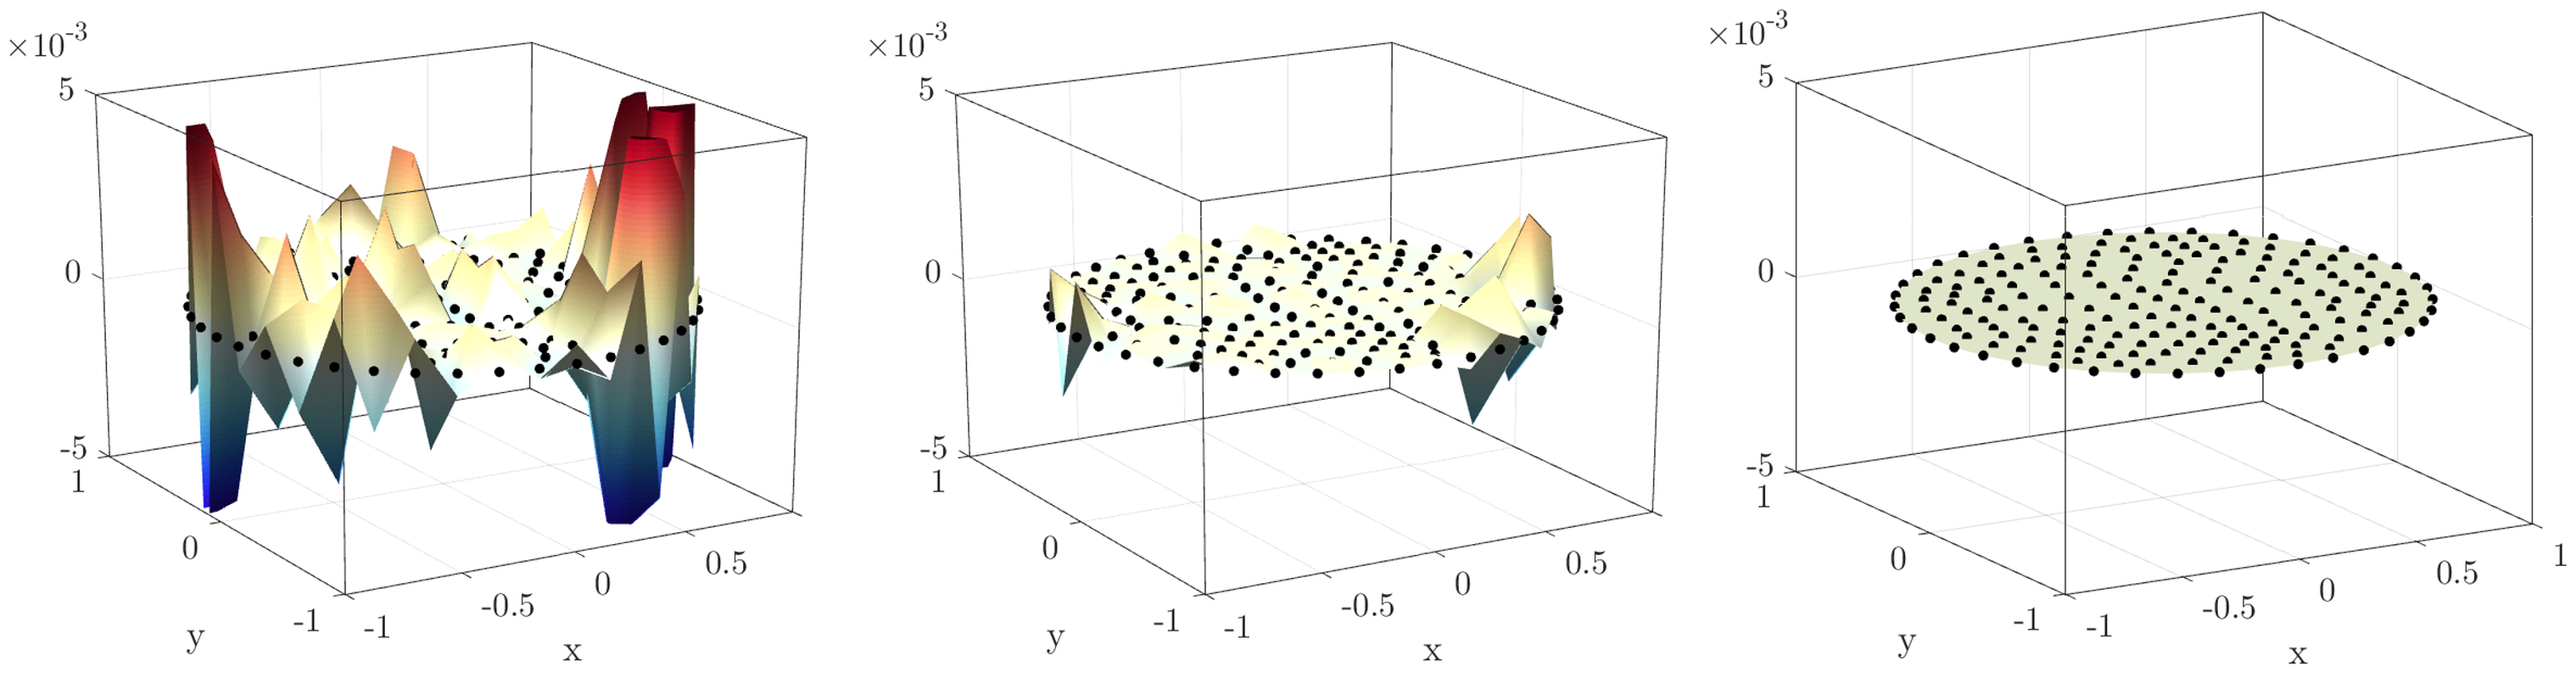
\includegraphics[width=\textwidth]{figs/fig01.png}
\caption{Examination of the 2nd order integration consistency for 2D cubic meshfree formulation.}\label{fig:1}
\end{figure}

\begin{figure}[pos=htbp]
\centering
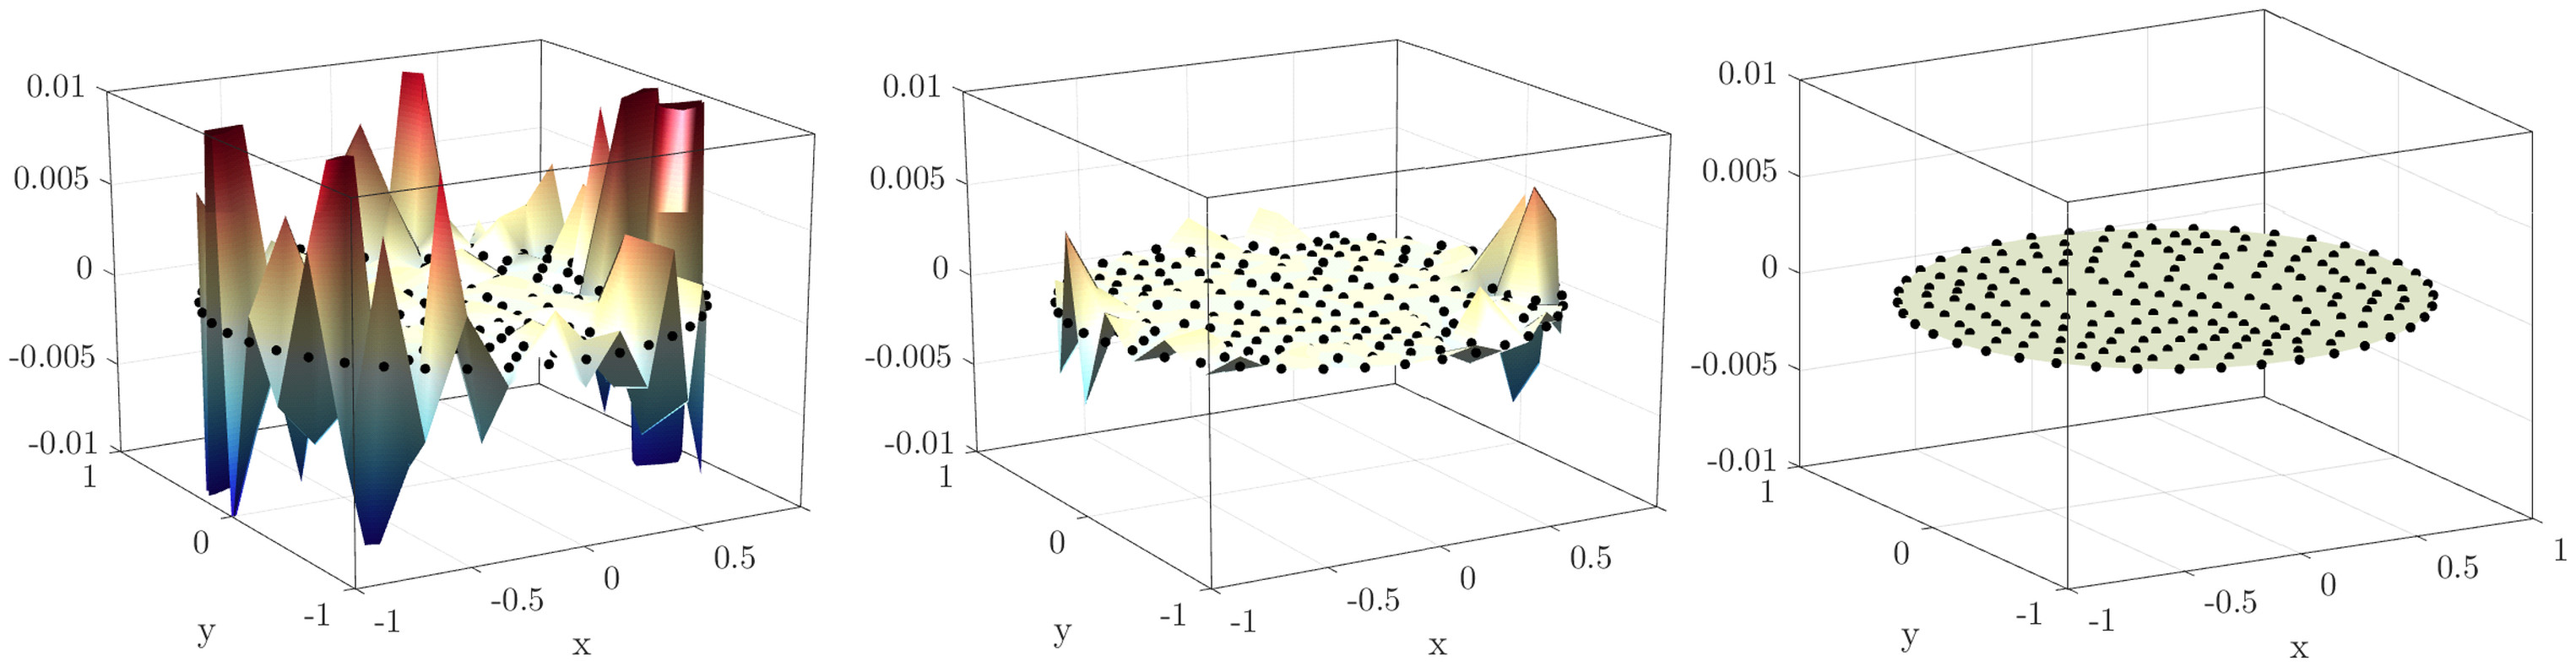
\includegraphics[width=\textwidth]{figs/fig02.png}
\caption{Examination of the 3rd order integration consistency for 2D cubic meshfree formulation.}\label{fig:2}
\end{figure}

\begin{figure}[pos=htbp]
\centering
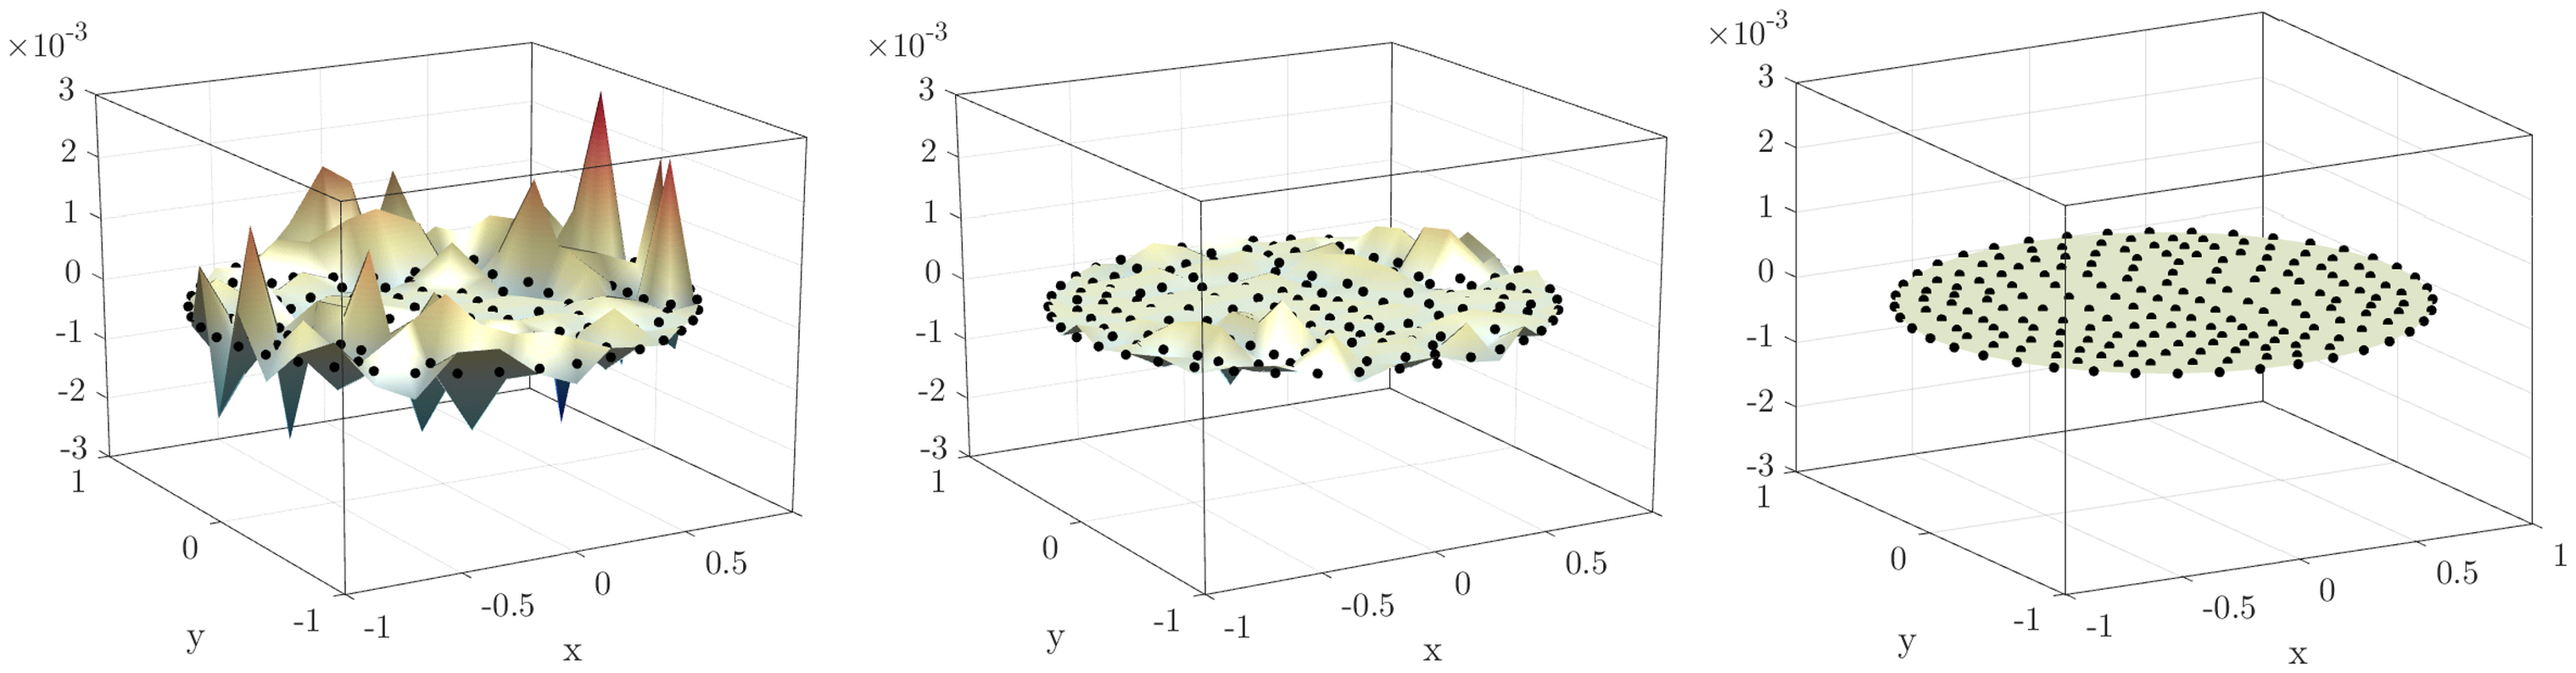
\includegraphics[width=\textwidth]{figs/fig03.png}
\caption{Examination of the 3rd order integration consistency for 2D quartic meshfree formulation.}\label{fig:3}
\end{figure}

\begin{figure}[pos=htbp]
\centering
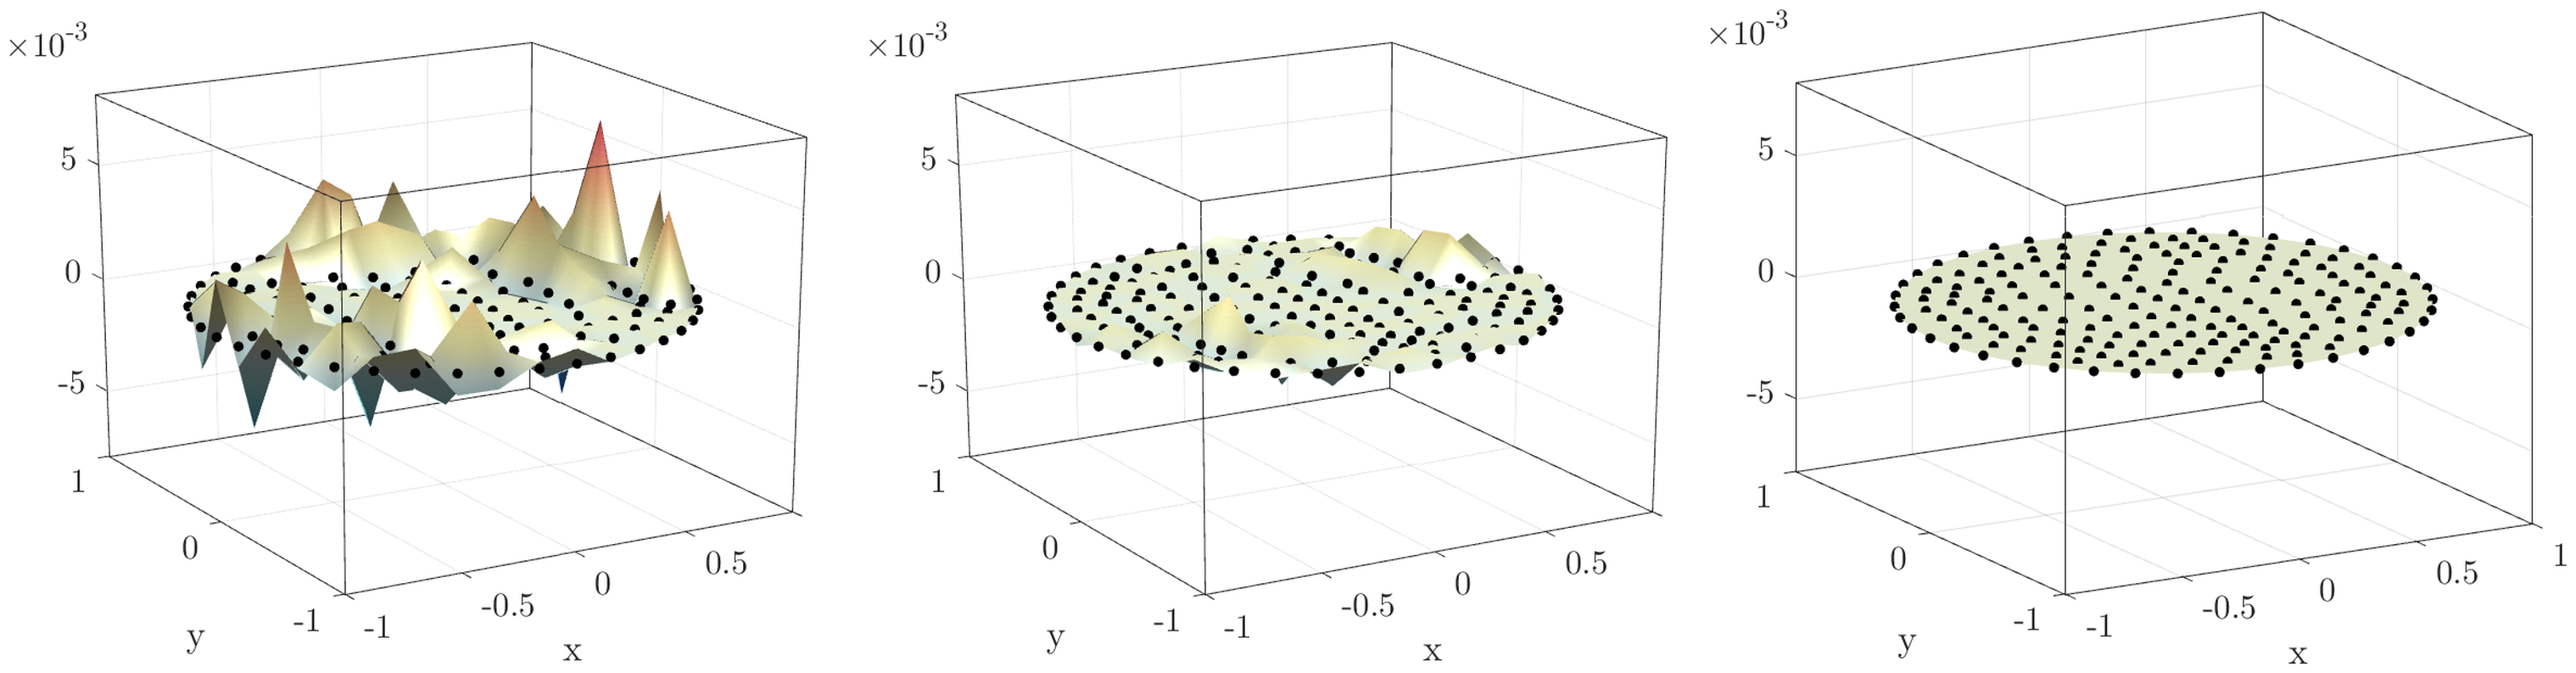
\includegraphics[width=\textwidth]{figs/fig04.png}
\caption{Examination of the 4th order integration consistency for 2D quartic meshfree formulation.}\label{fig:4}
\end{figure}

Figs. \ref{fig:1}--\ref{fig:4} clearly show the various orders of integration consistency of GI and RKGSI for cubic and quartic basis function.
Since RKGSI was generated from integration constraints of weak forms regarding to various orders $q$ of meshfree formulations, it naturally possess the integration consistency the same degree of basis functions.

\subsection{Examination for convergence rates of quadratic meshfree formulation}\label{sec:quadratic}

As stated in Section \ref{sec:error}, only when the order of basis function satisfy the minimum requirement $p\ge3$, can the $L_2$ error of various integral schemes achieves optimal convergence performance $p+1$, otherwise, only $p$th order convergence rate of $L_2$ error can be ensured when $p=2$.
Then two benchmark problems will be adopted to test the above theoretical convergence value.

We consider a 1D cantilever beam as shown in Fig. \ref{fig:5}.
The analytical solution and corresponding boundary conditions are as follows:
\begin{equation}\label{eq:90}
\begin{cases}
w=\sin x-x\\[2pt]
w(0)=0,\quad \theta(0)=0
\end{cases}
\end{equation}
The material and geometry properties of this problem are: flexural rigidity $D=2\times10^{4}$, Poisson's ratio $\nu=0.3$, length $L=10$.
The left boundary is subject to displacement and rotation boundary conditions, which are imposed by Nitsche's method.
Six regular meshfree discretizations with $11$, $21$, $41$, $81$, $161$, $321$ nodes are adopted to observe the convergence performance.
For quadratic meshfree computation, the normalized support size is set as 2.6.

\begin{figure}[pos=htbp]
\centering
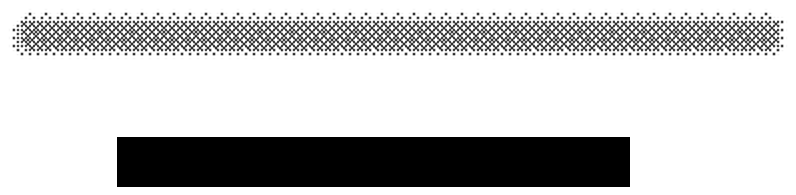
\includegraphics[width=0.7\textwidth]{figs/fig05.png}
\caption{Description of 1D cantilever beam.}\label{fig:5}
\end{figure}

\begin{figure}[pos=htbp]
\centering
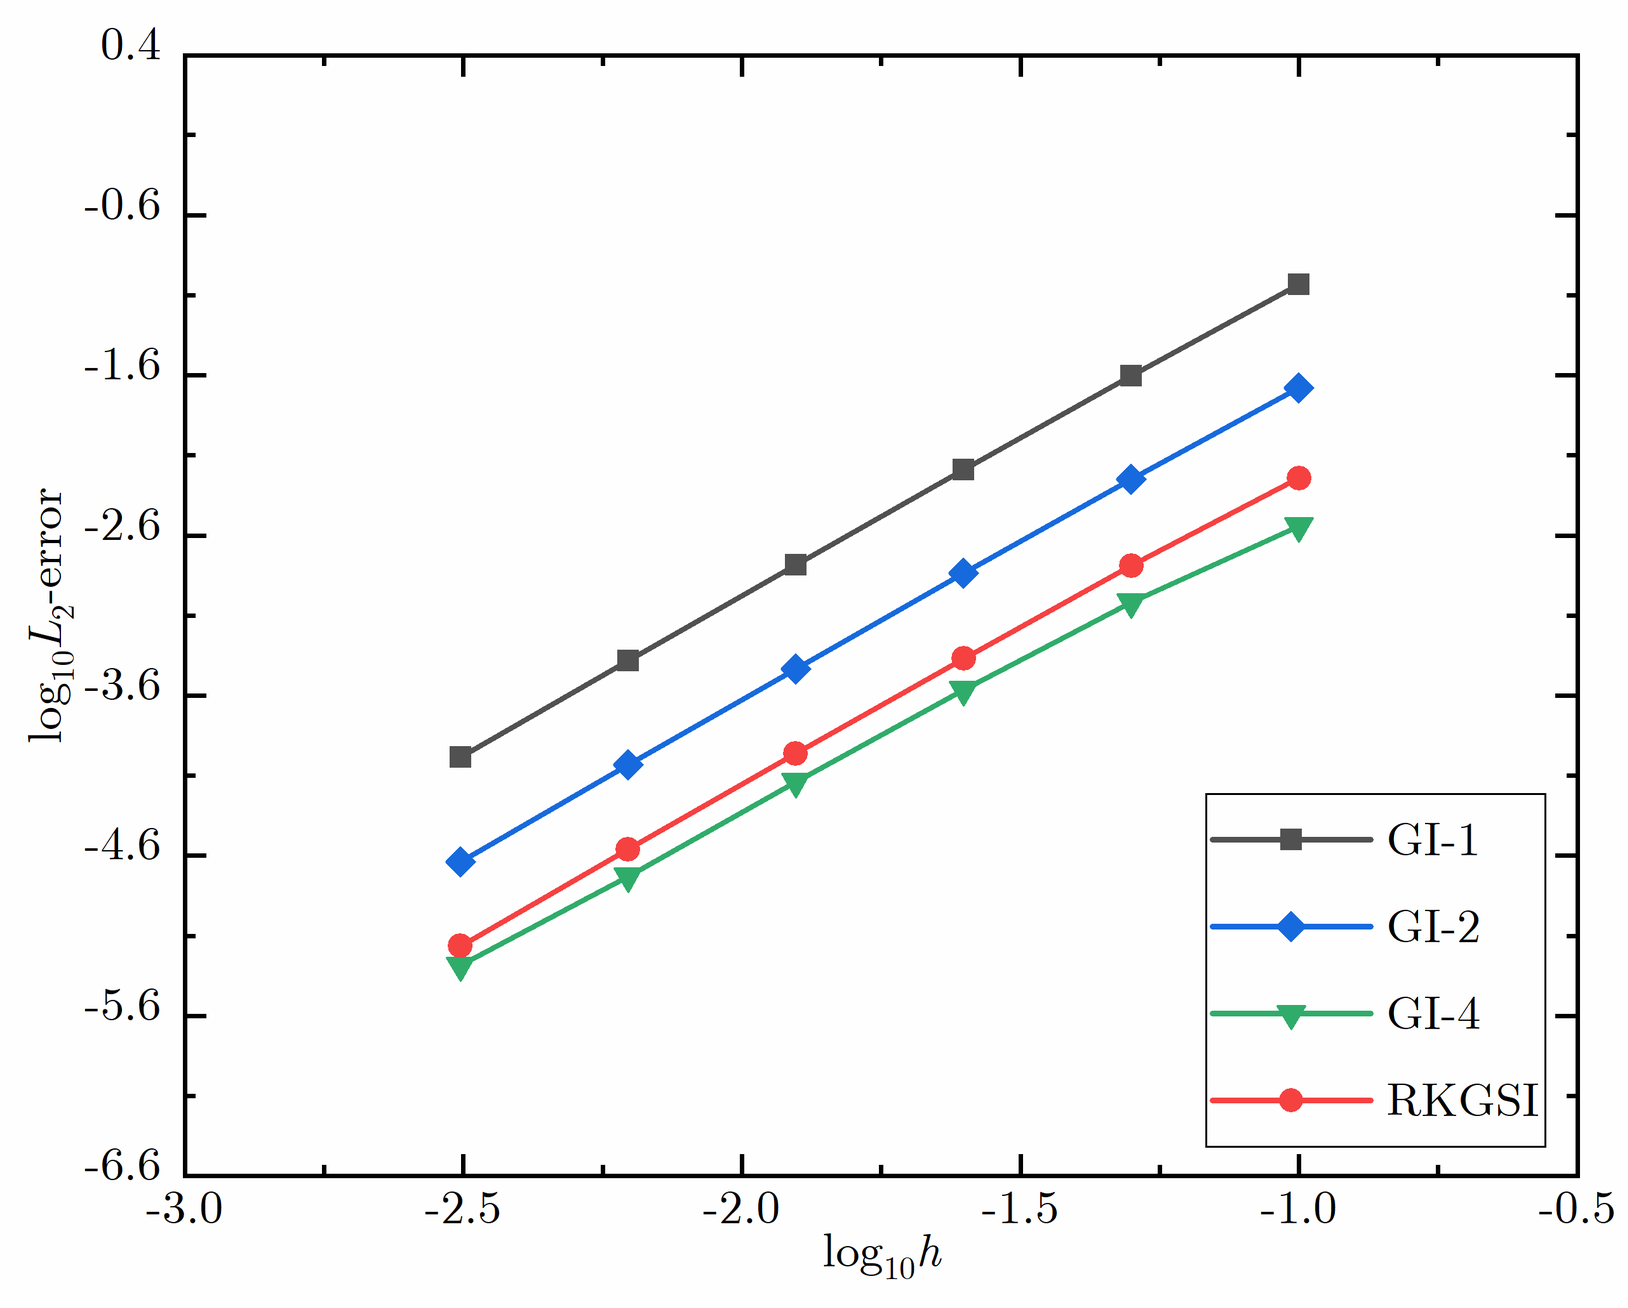
\includegraphics[width=0.55\textwidth]{figs/fig06.png}
\caption{$L_2$-error comparison for the 1D cantilever beam with $p=2$.}\label{fig:6}
\end{figure}

\begin{figure}[pos=htbp]
\centering
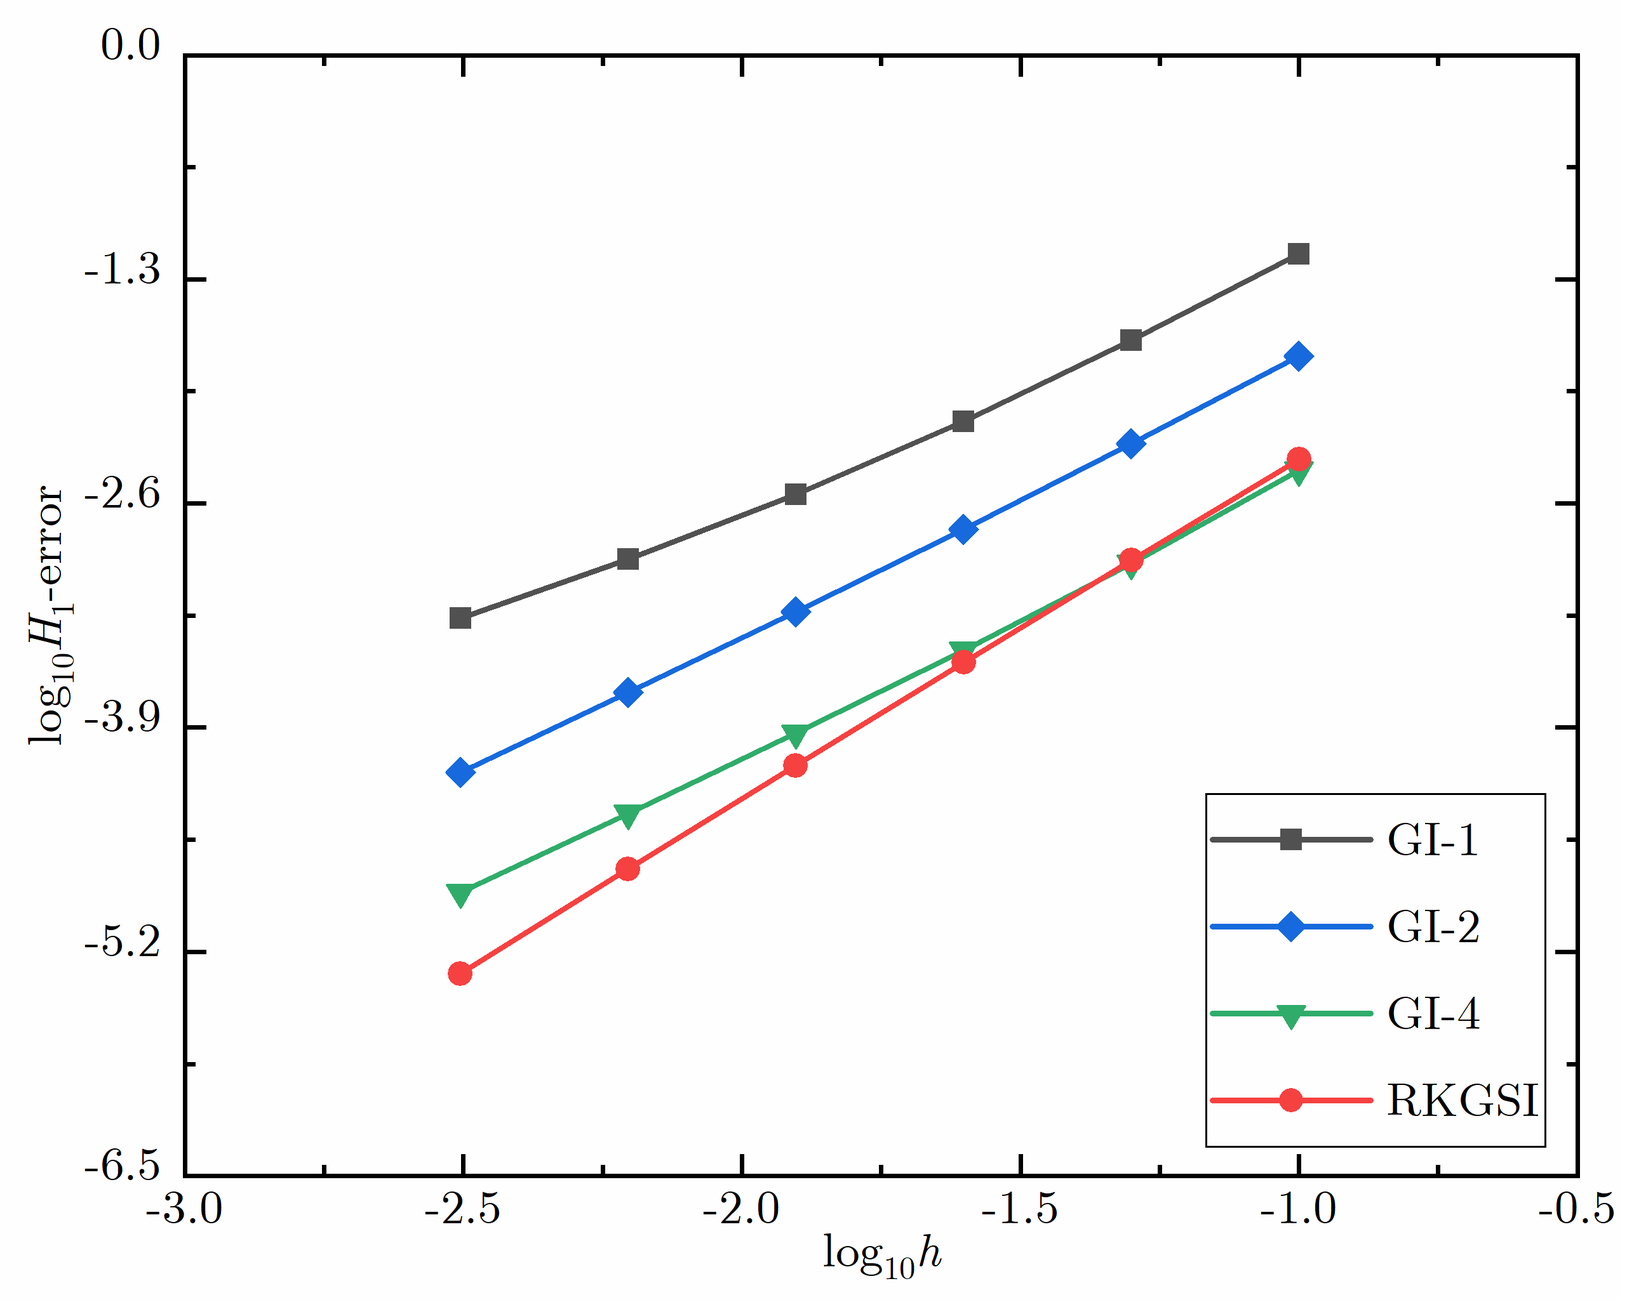
\includegraphics[width=0.55\textwidth]{figs/fig07.png}
\caption{$H_1$-error comparison for the 1D cantilever beam with $p=2$.}\label{fig:7}
\end{figure}

\begin{figure}[pos=htbp]
\centering
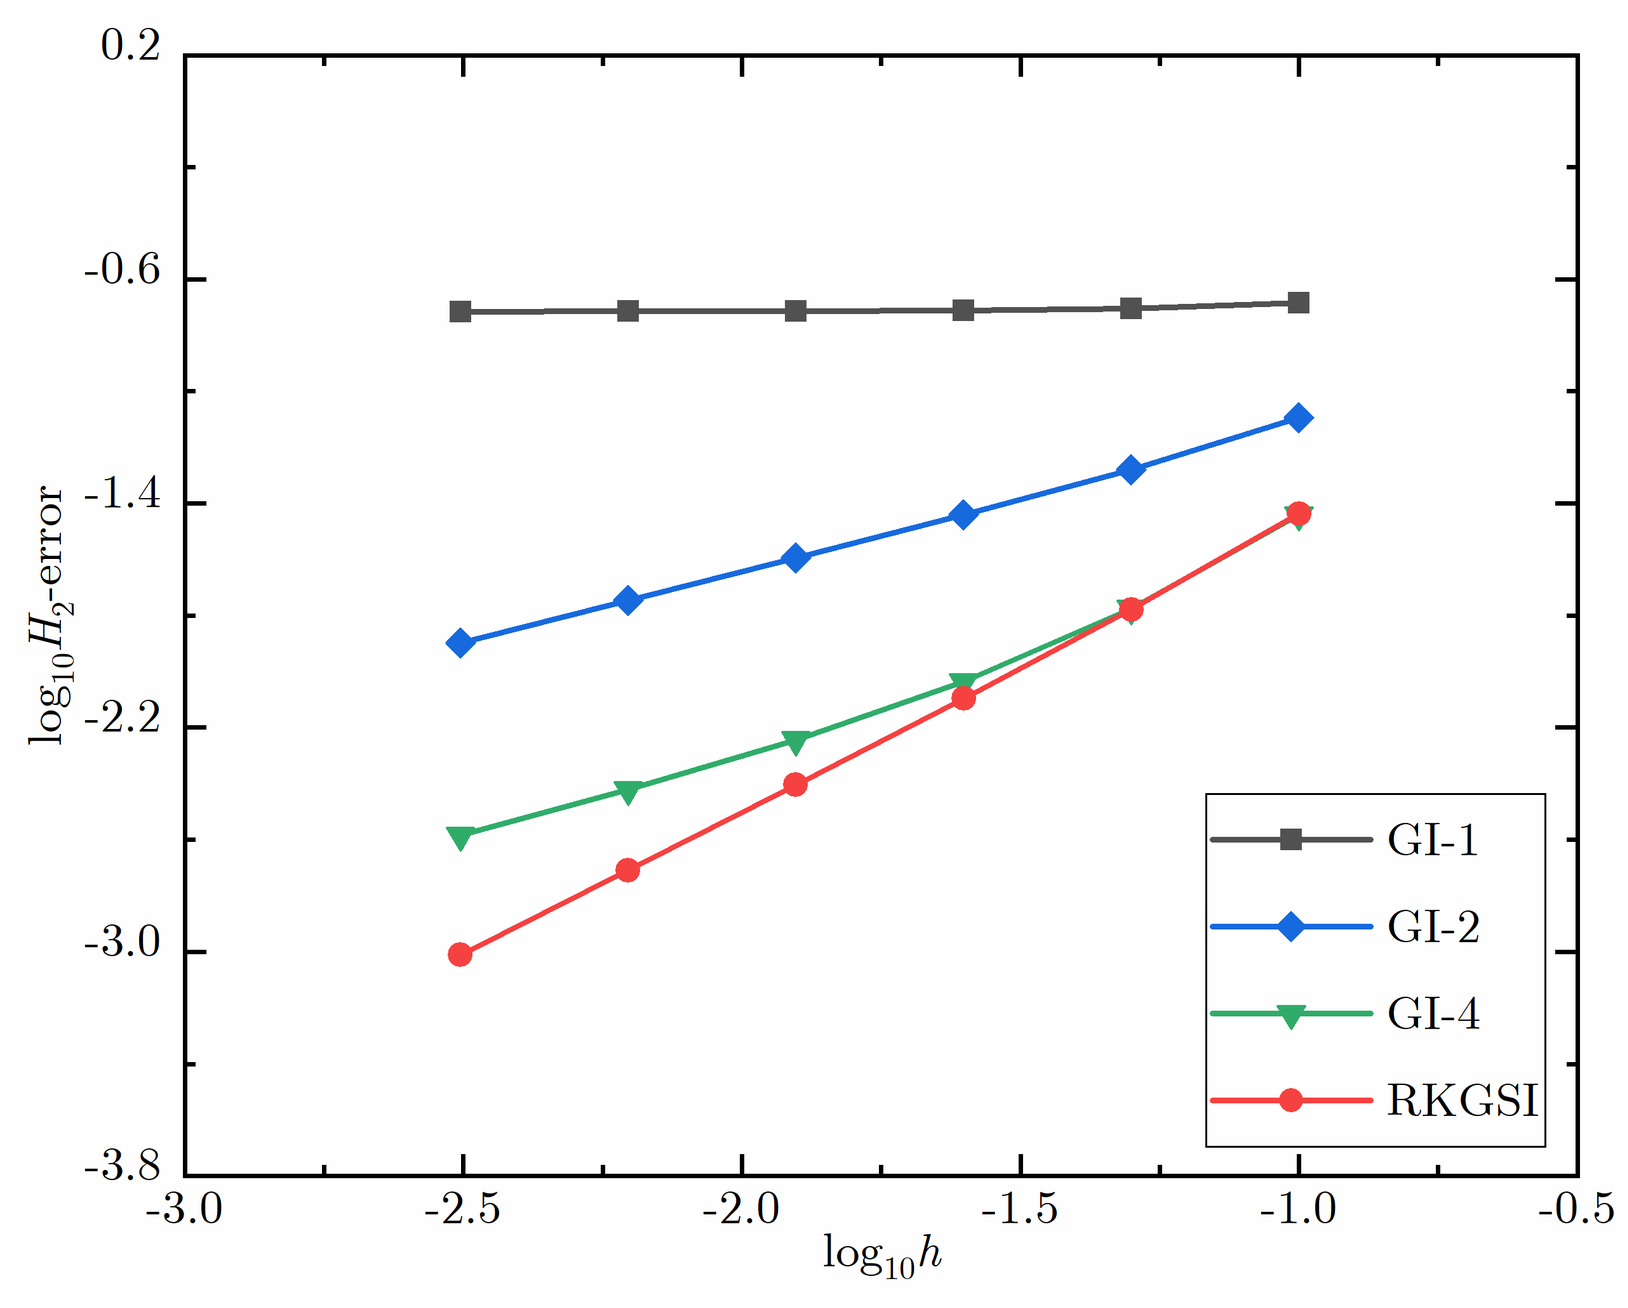
\includegraphics[width=0.55\textwidth]{figs/fig08.png}
\caption{$H_2$-error comparison for the 1D cantilever beam with $p=2$.}\label{fig:8}
\end{figure}

Figs. \ref{fig:6}--\ref{fig:8} show the convergence rates of compute error regarding to $L_2$, $H_1$ and $H_2$ norm for Gauss integration based methods (GI-1, 2, 4) and reproducing kernel gradient smoothing integration based method (RKGSI).
It clearly evinces the importance of the order of basis function, when $p=2$, all the integral schemes both ensure second order of convergence for $L_2$ error even though RKGSI possess the same order of integration consistency as basis function ($q=p=2$), while the integration consistency of GI only be $q=1$.
For $H_1$ and $H_2$ error in Figs. \ref{fig:7} and \ref{fig:8}, notable advantages of RKGSI can be observed with smaller nodal distances, which originates from deficiency of integration consistency of GI.

Another 2D benchmark problem is a left-clamped plate shown in Fig. \ref{fig:9}, whose material properties is the same as the previous 1D beam, geometry property is $L_x=L_y=1$.
The analytical solution and boundary conditions are given by:
\begin{equation}\label{eq:91}
\begin{cases}
w=\left(\sin x-x\right)\left(y+y^{2}\right)\\[2pt]
w(0,y)=0,\quad \theta(0,y)=0
\end{cases}
\end{equation}

\begin{figure}[pos=htbp]
\centering
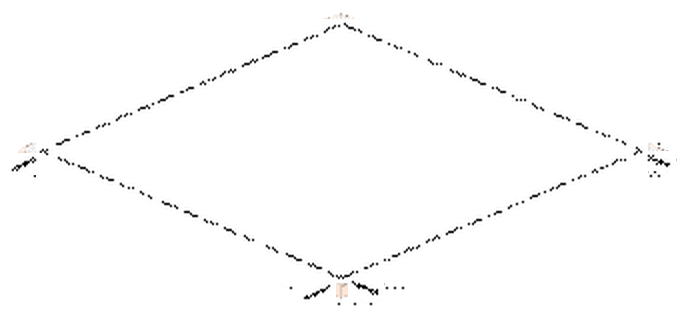
\includegraphics[width=0.6\textwidth]{figs/fig09.png}
\caption{Description of left-clamped plate.}\label{fig:9}
\end{figure}

\begin{figure}[pos=htbp]
\centering
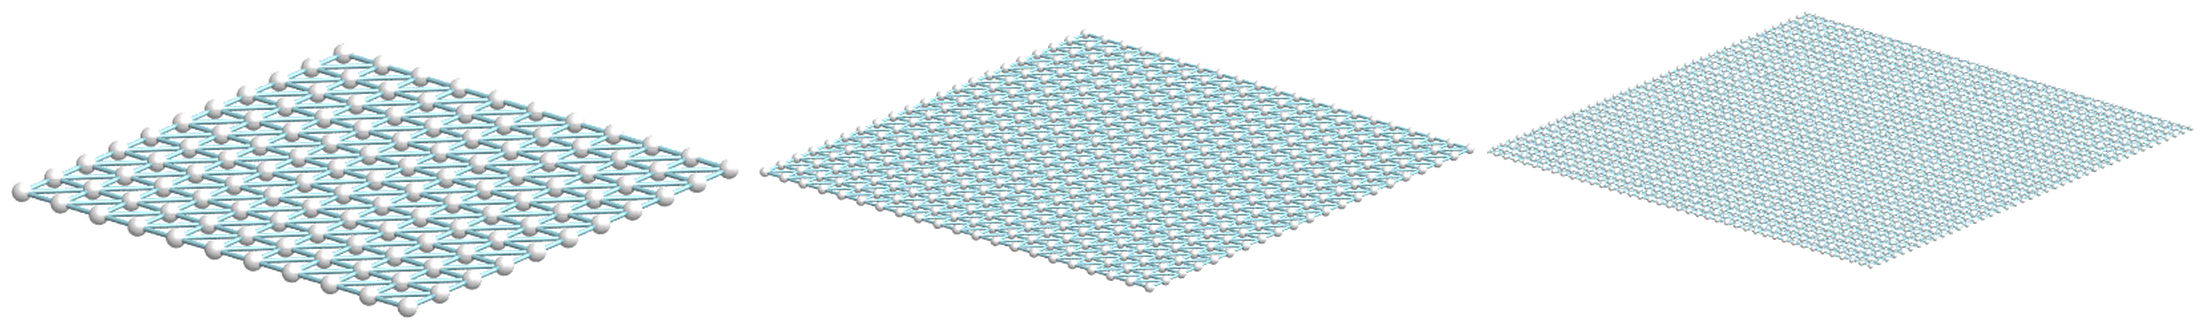
\includegraphics[width=\textwidth]{figs/fig10.png}
\caption{Meshfree discretizations with 36, 121, 441 nodes.}\label{fig:10}
\end{figure}

The normalized support size for quadratic meshfree formulation is set as 2.6.
As shown in Fig. \ref{fig:10}, five regular meshfree discretizations with 36, 121, 441, 1681, 6561 nodes are employed in order to observe the numerical convergence rates of GI and RKGSI.
The convergence performances listed in Figs. \ref{fig:11}--\ref{fig:13} further confirm the theoretical conclusion, which is, when $p=2$, the $L_2$, $H_1$ and $H_2$ errors of RKGSI with $q=p$ respectively converge at the rate of 2, 2 and 1 under refining discretizations, while the convergence rates of GI only achieves about 2, 1 and 0 due to a smaller order of integration consistency than basis function ($q<p$) in traditional Galerkin meshfree methods (such as GI-3, 6 and 9).

\begin{figure}[pos=htbp]
\centering
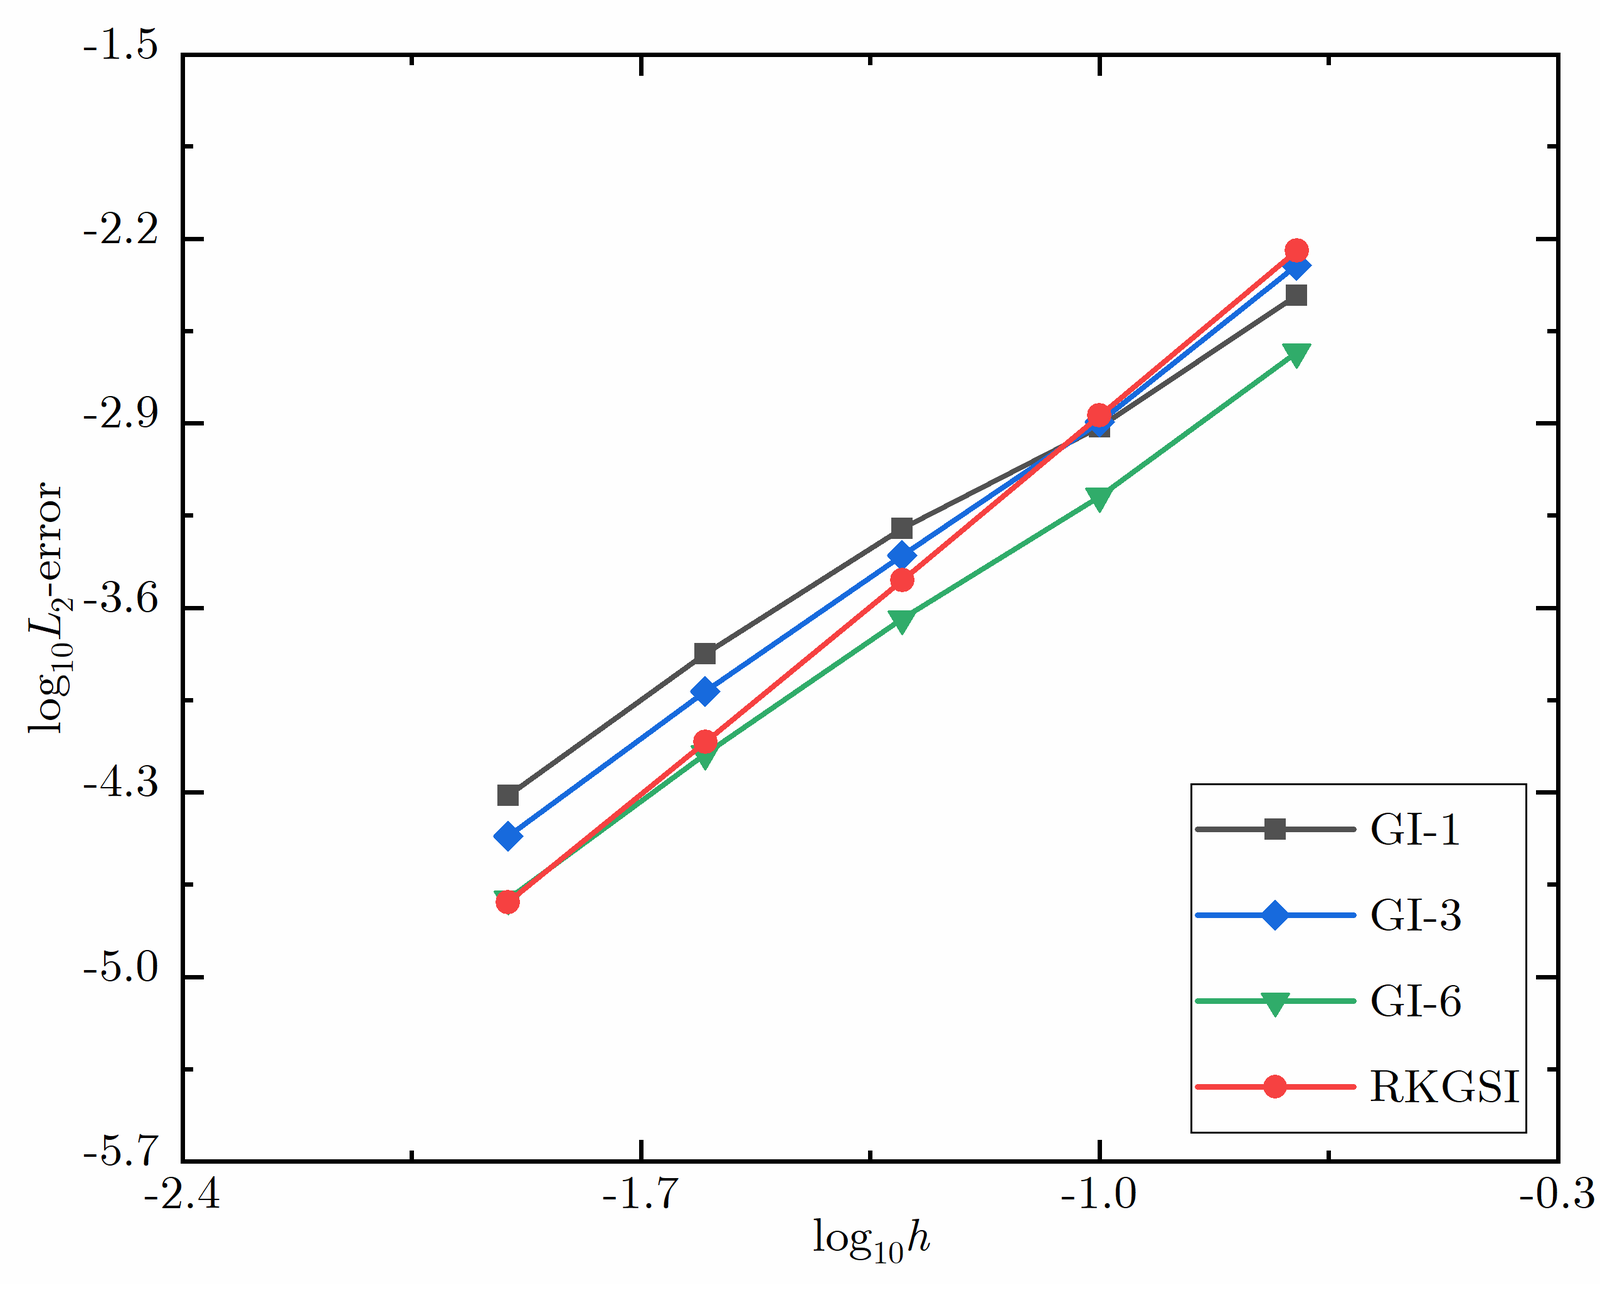
\includegraphics[width=0.55\textwidth]{figs/fig11.png}
\caption{$L_2$-error comparison for the 2D singly clamped plate with $p=2$.}\label{fig:11}
\end{figure}

\begin{figure}[pos=htbp]
\centering
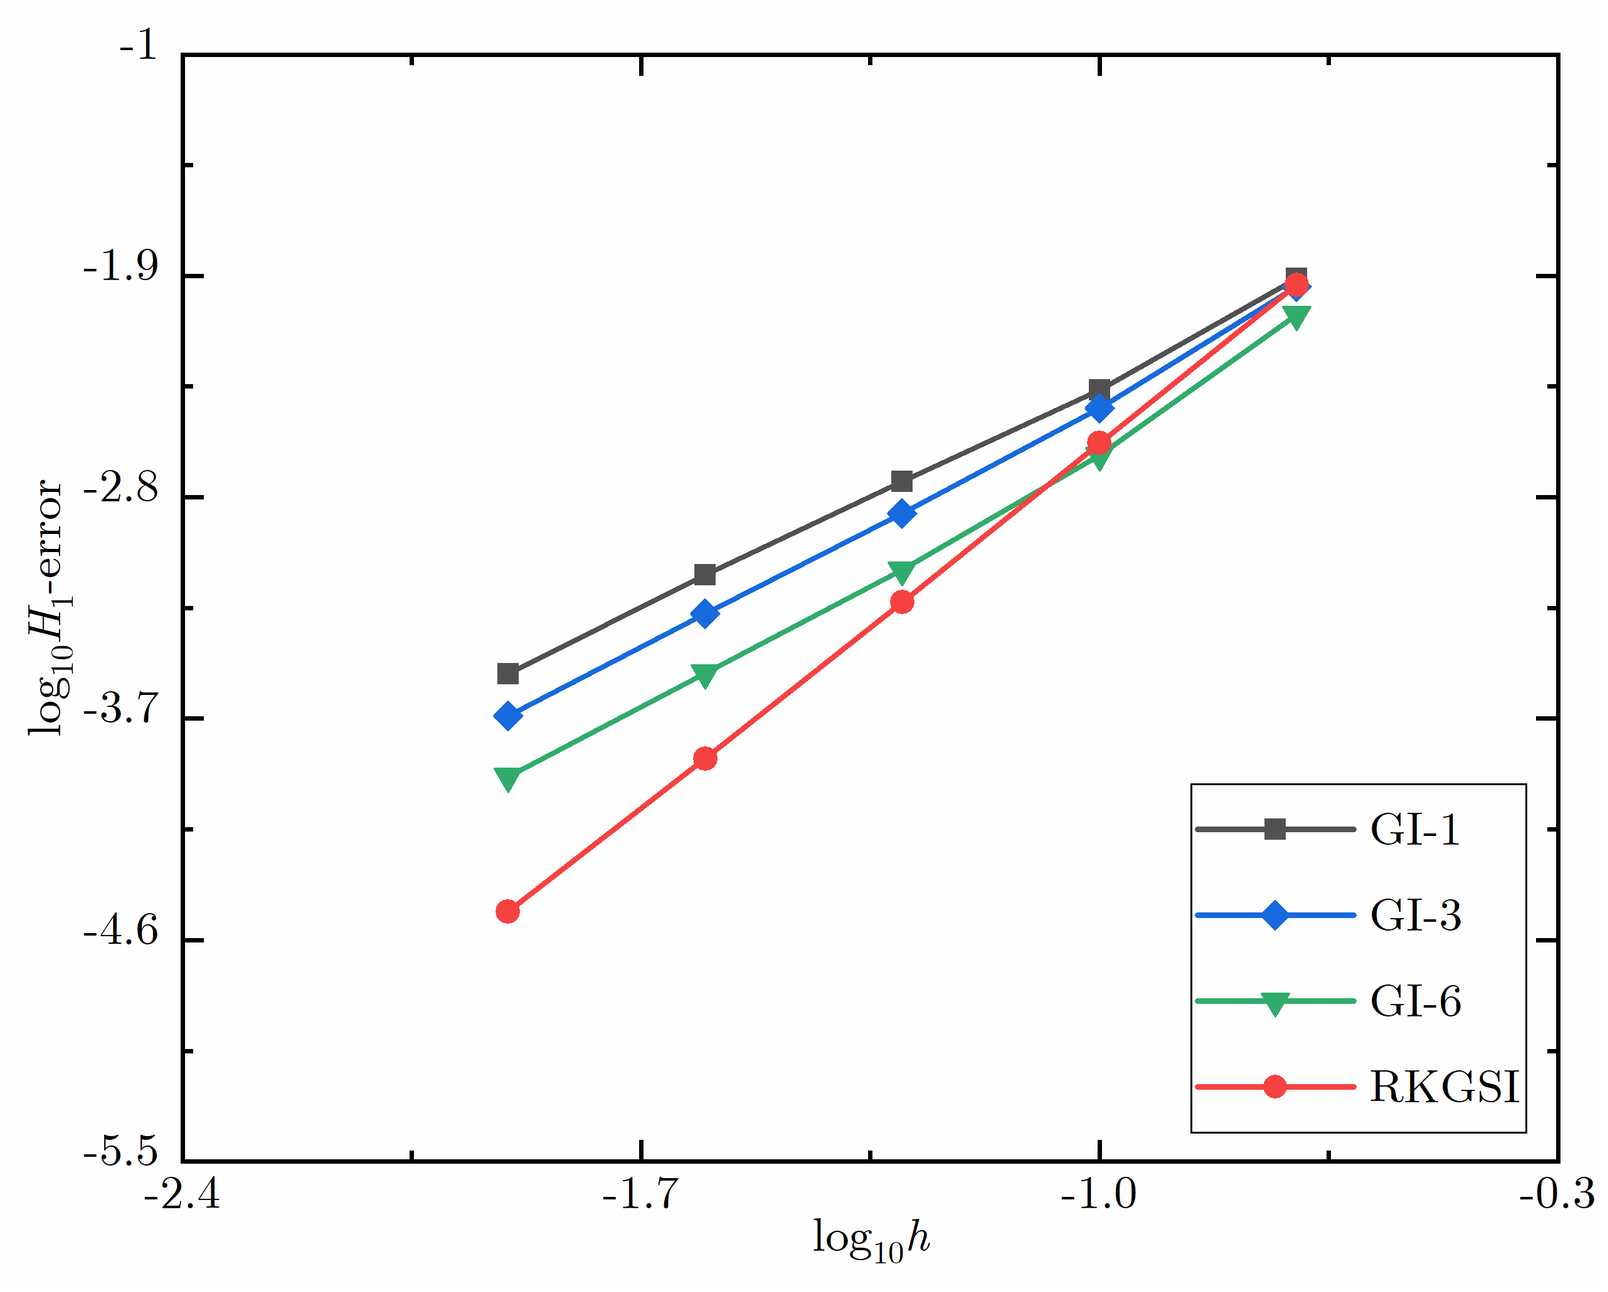
\includegraphics[width=0.55\textwidth]{figs/fig12.png}
\caption{$H_1$-error comparison for the 2D singly clamped plate with $p=2$.}\label{fig:12}
\end{figure}

\begin{figure}[pos=htbp]
\centering
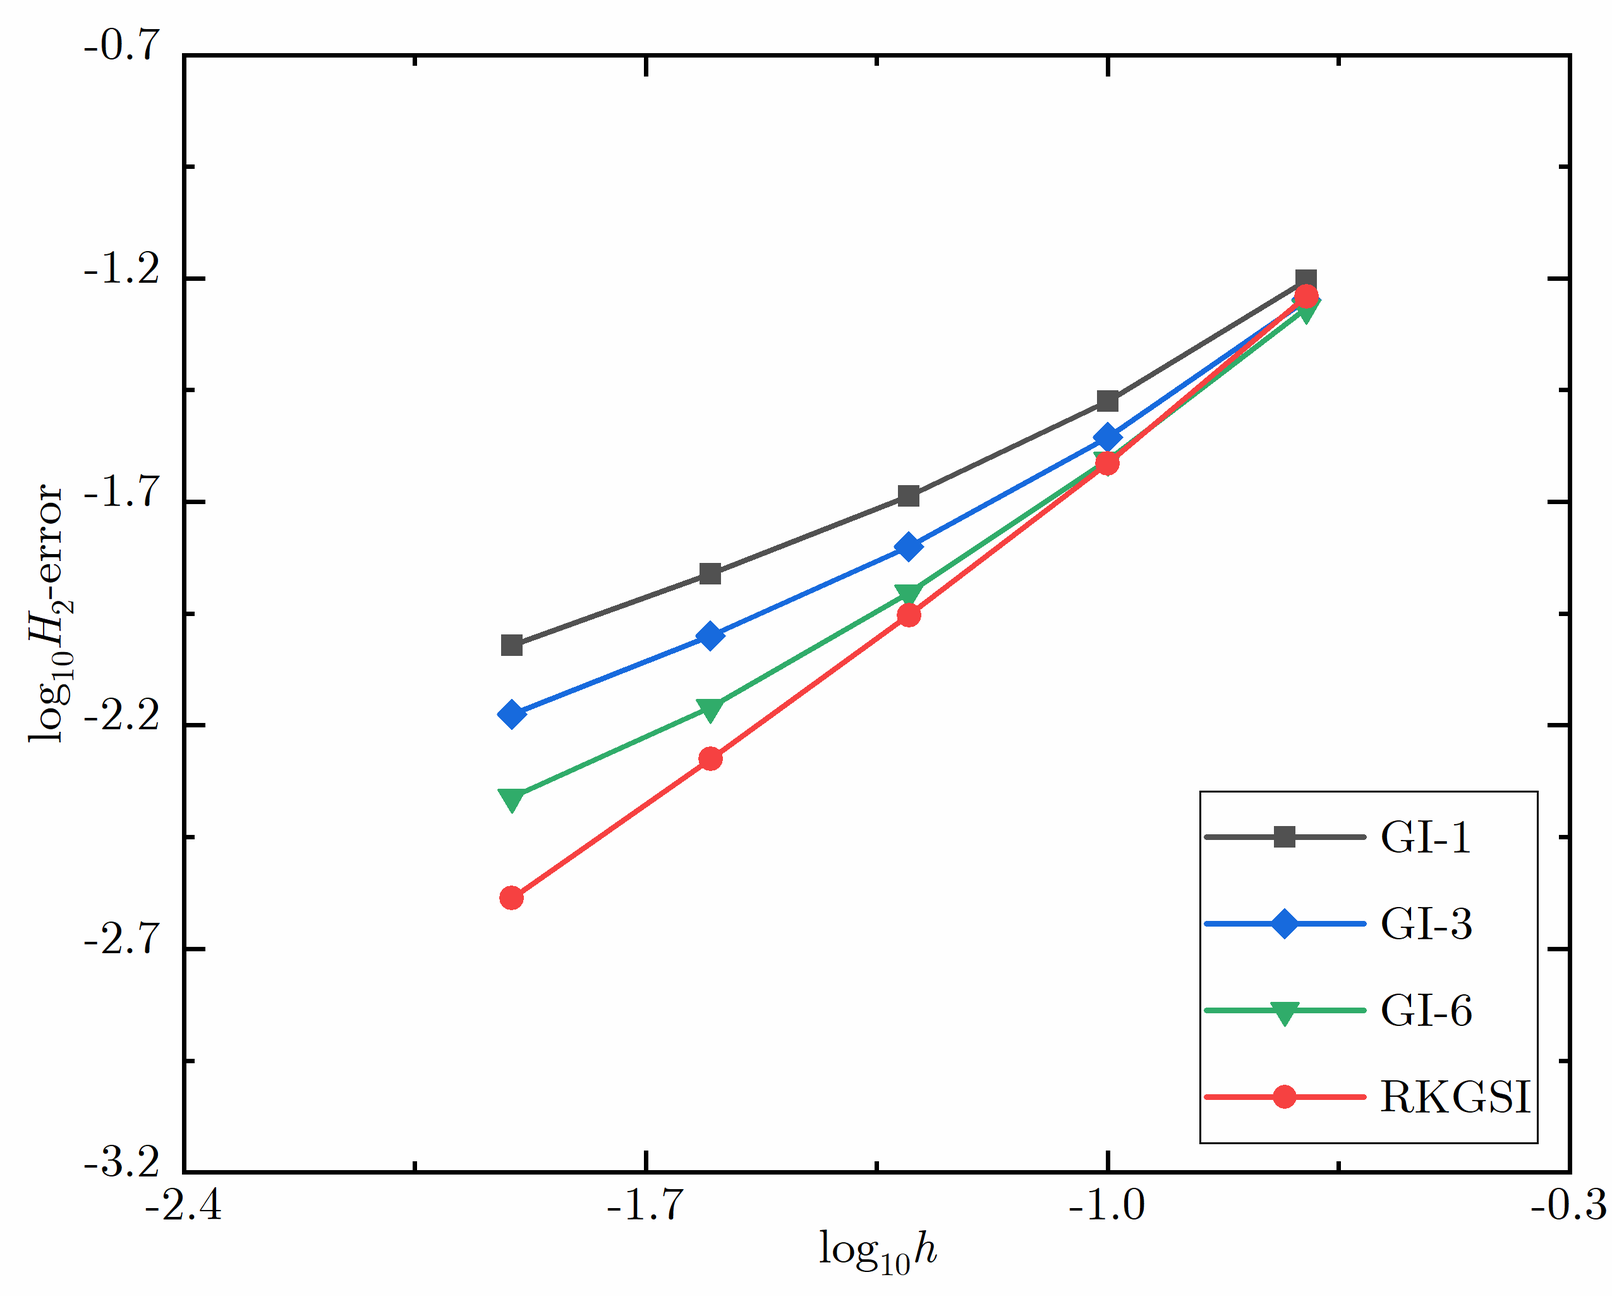
\includegraphics[width=0.55\textwidth]{figs/fig13.png}
\caption{$H_2$-error comparison for the 2D singly clamped plate with $p=2$.}\label{fig:13}
\end{figure}

For better illustrating the importance of integration consistency, in subsequent contents, we will focus on cubic and quartic meshfree formulation with GI and RGKSI.

\subsection{1D manufactured beam}\label{sec:manufactured1d}

In order to assess the convergence performance of Galerkin meshfree methods with cubic and quartic basis function, we consider a manufactured beam as shown in Fig. \ref{fig:14}, and an octal polynomial solution is employed to perform the meshfree computation:
\begin{equation}\label{eq:92}
w=x^{8}/100+2x^{7}/100+x^{6}+x^{5}+5x^{4}+3x^{3}+4x^{2}+5x+6
\end{equation}
All specific values of boundary conditions are determined by Eq. \eqref{eq:92}.
The displacement and moment boundary conditions are imposed on both sides.
Also, the material and geometry properties are the same as 1D cantilever beam in Section \ref{sec:quadratic}.

\begin{figure}[pos=htbp]
\centering
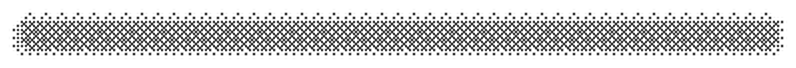
\includegraphics[width=0.85\textwidth]{figs/fig14.png}
\caption{Description of 1D manufactured beam.}\label{fig:14}
\end{figure}

Five meshfree discretizations with 11, 21, 41, 81, 161 nodes are adopted to observe the convergence performance.
For meshfree computation, the normalized support sizes are respectively prescribed as 3.5 and 4.5 for $p=3,4$.
The convergence results referring to $L_2$, $H_1$ and $H_2$ error norms for cubic and quartic meshfree formulation are listed in Figs. \ref{fig:15}--\ref{fig:20}, respectively.
The results clearly show that the convergence rates of GI-3, GI-6 and GI-9 adopted in cubic meshfree formulation, GI-4, GI-8 and GI-13 adopted in quartic meshfree formulation both are 2, 1, 0, respectively.
This is because Gauss integration can not meet the cubic and quartic integration constraints corresponding to the orders of basis functions, i.e., the integration consistency of GI is $q=1$, which is lower than $p$, thus the integration error totally governs the convergence performance of Galerkin meshfree methods with the nodal distance constantly decreasing.
On the contrary, according to the previous description, since RKGSI based meshfree formulation possess corresponding integration consistency $q=p$, it is capable for producing optimal convergence rates of $L_2$, $H_1$ and $H_2$ error norms, which respectively are 4, 3 and 2 in cubic case, 5, 4, 3 in quartic case.

\begin{figure}[pos=htbp]
\centering
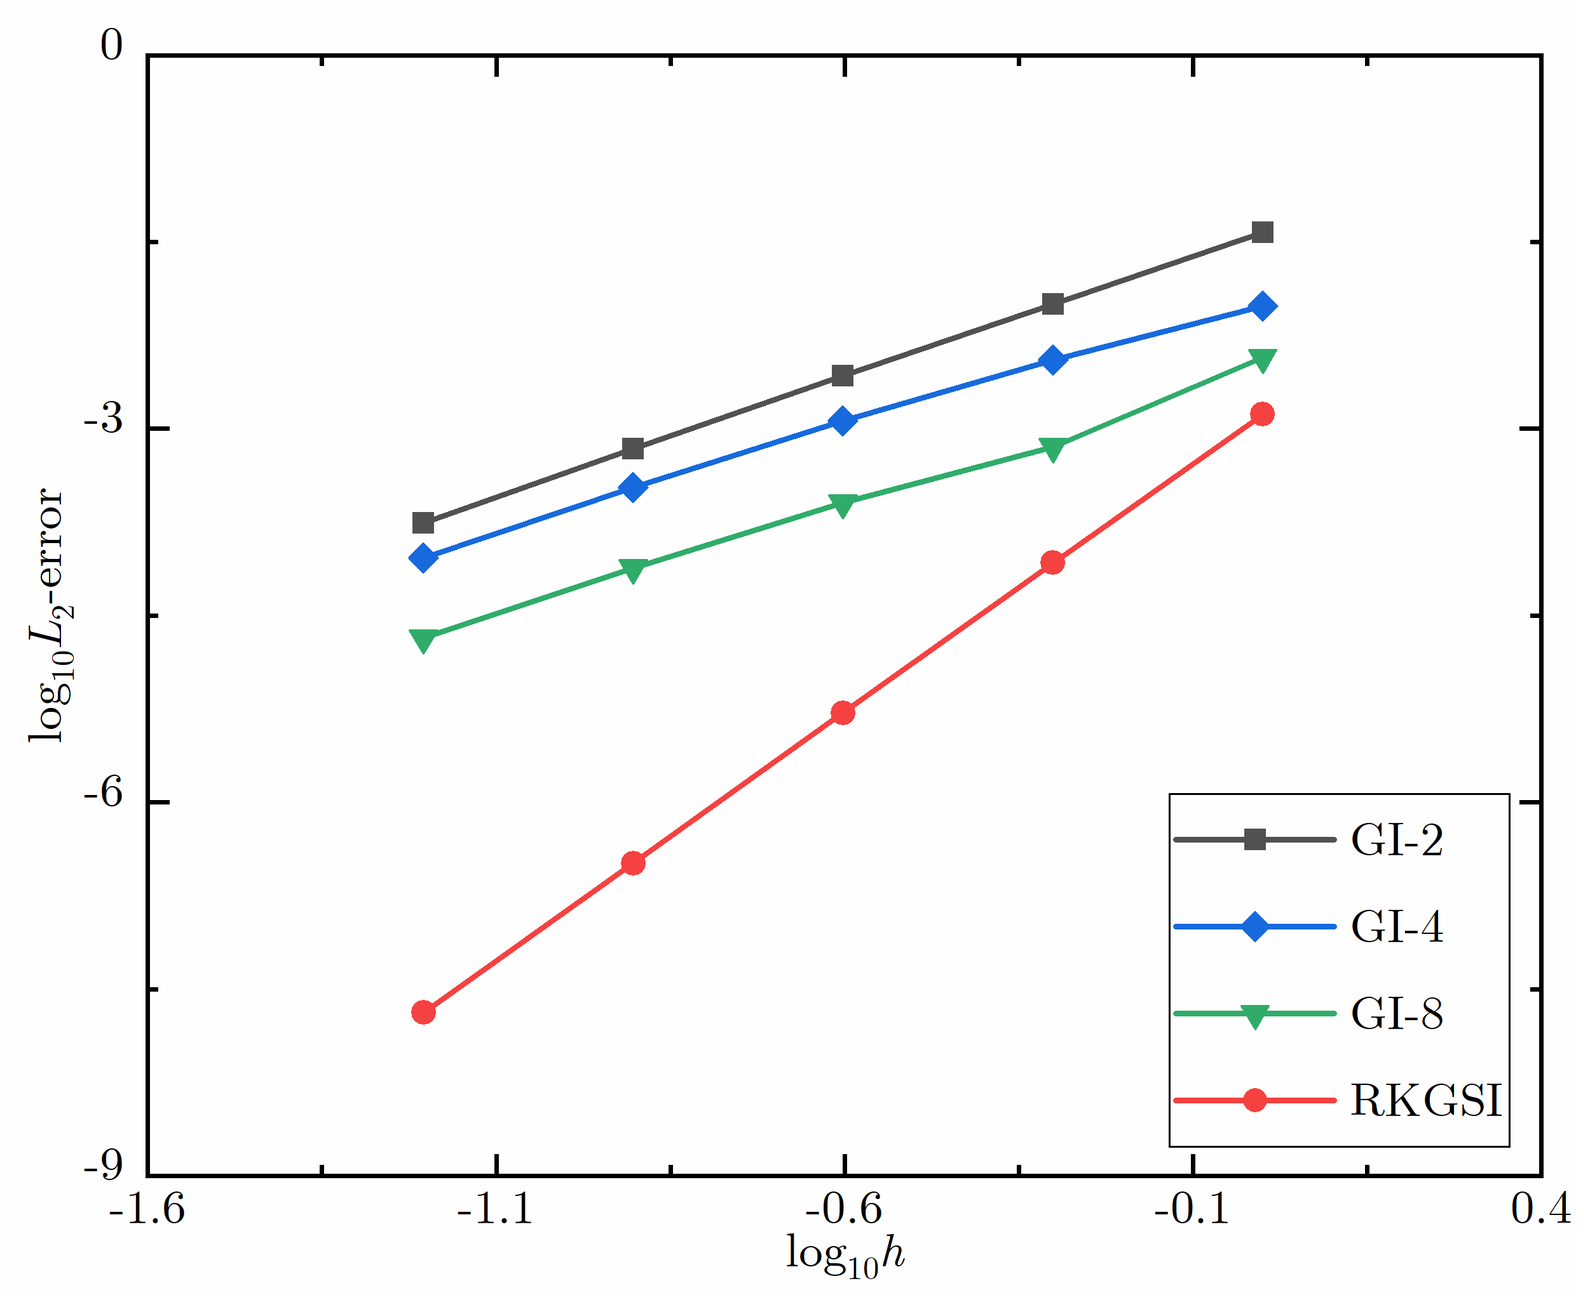
\includegraphics[width=0.55\textwidth]{figs/fig15.png}
\caption{$L_2$-error comparison for the 1D manufactured beam with $p=3$.}\label{fig:15}
\end{figure}

\begin{figure}[pos=htbp]
\centering
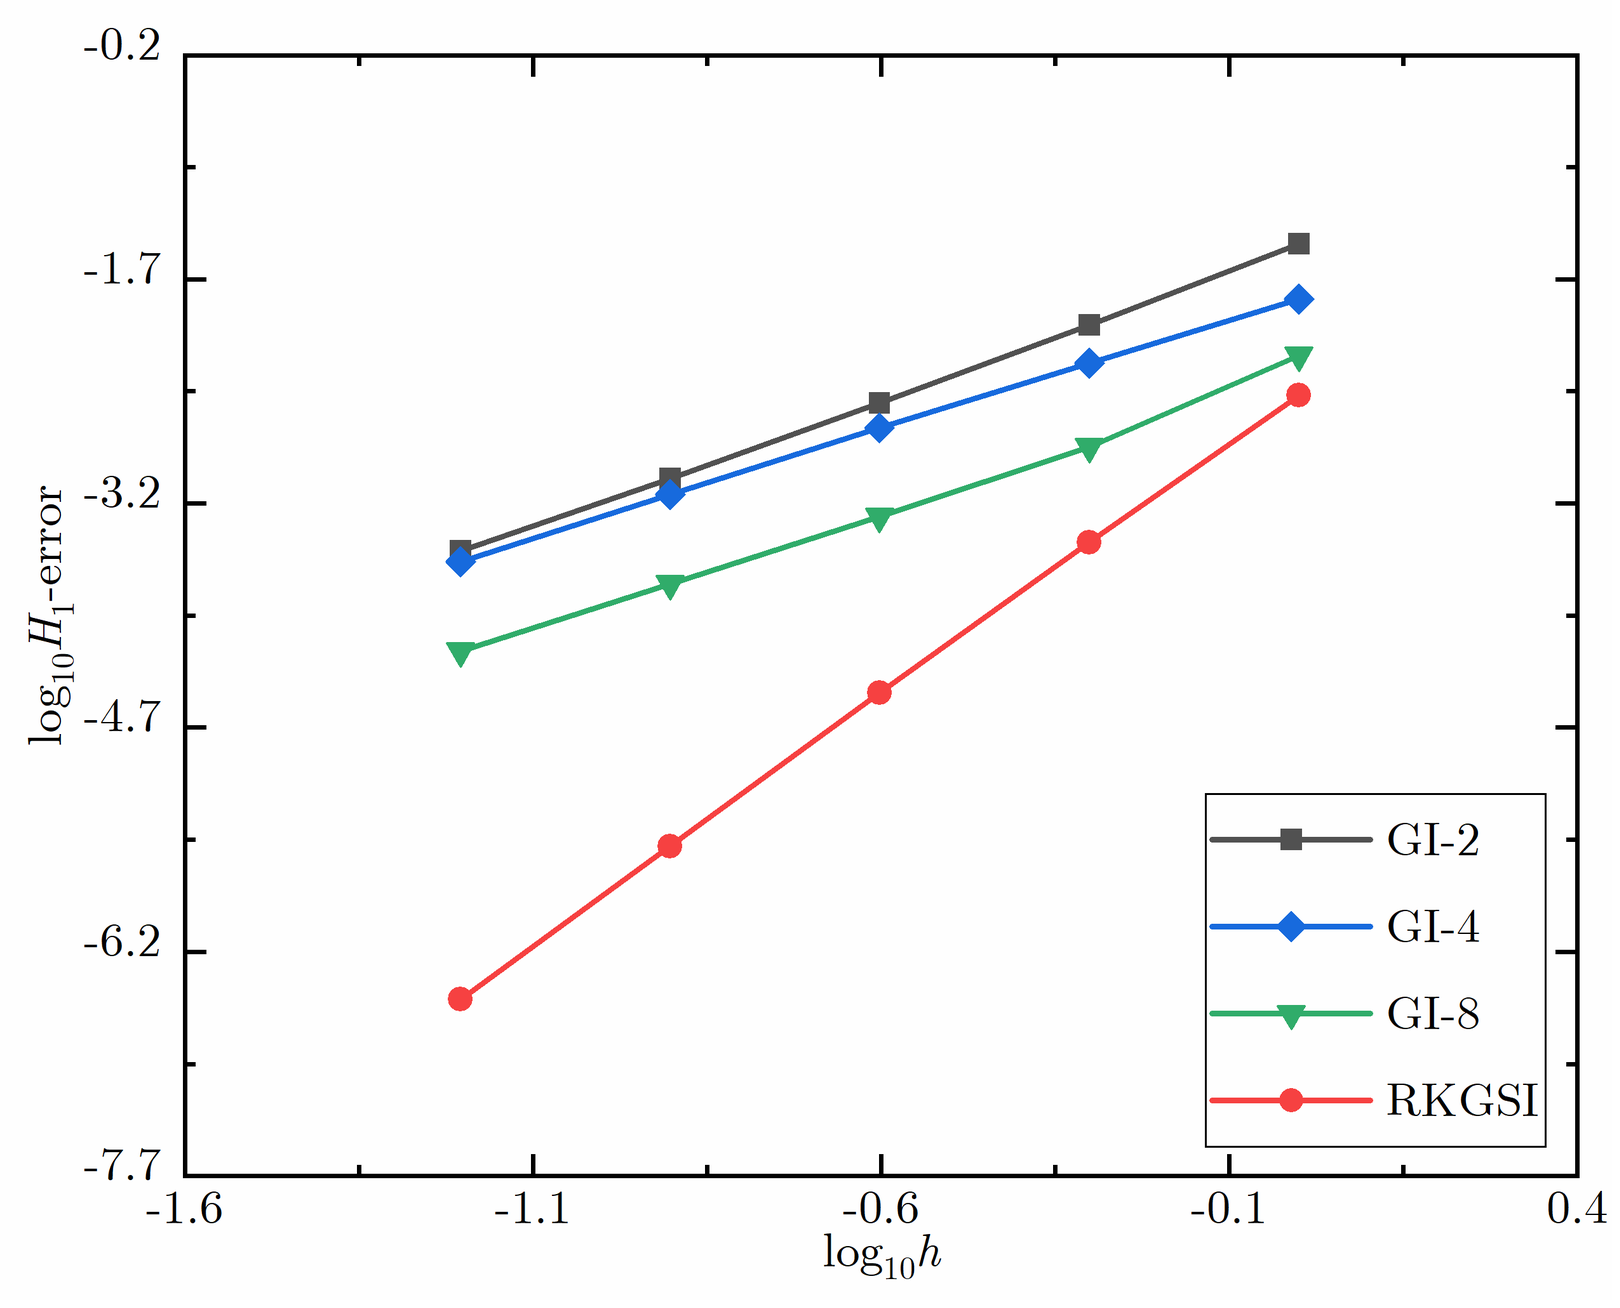
\includegraphics[width=0.55\textwidth]{figs/fig16.png}
\caption{$H_1$-error comparison for the 1D manufactured beam with $p=3$.}\label{fig:16}
\end{figure}

\begin{figure}[pos=htbp]
\centering
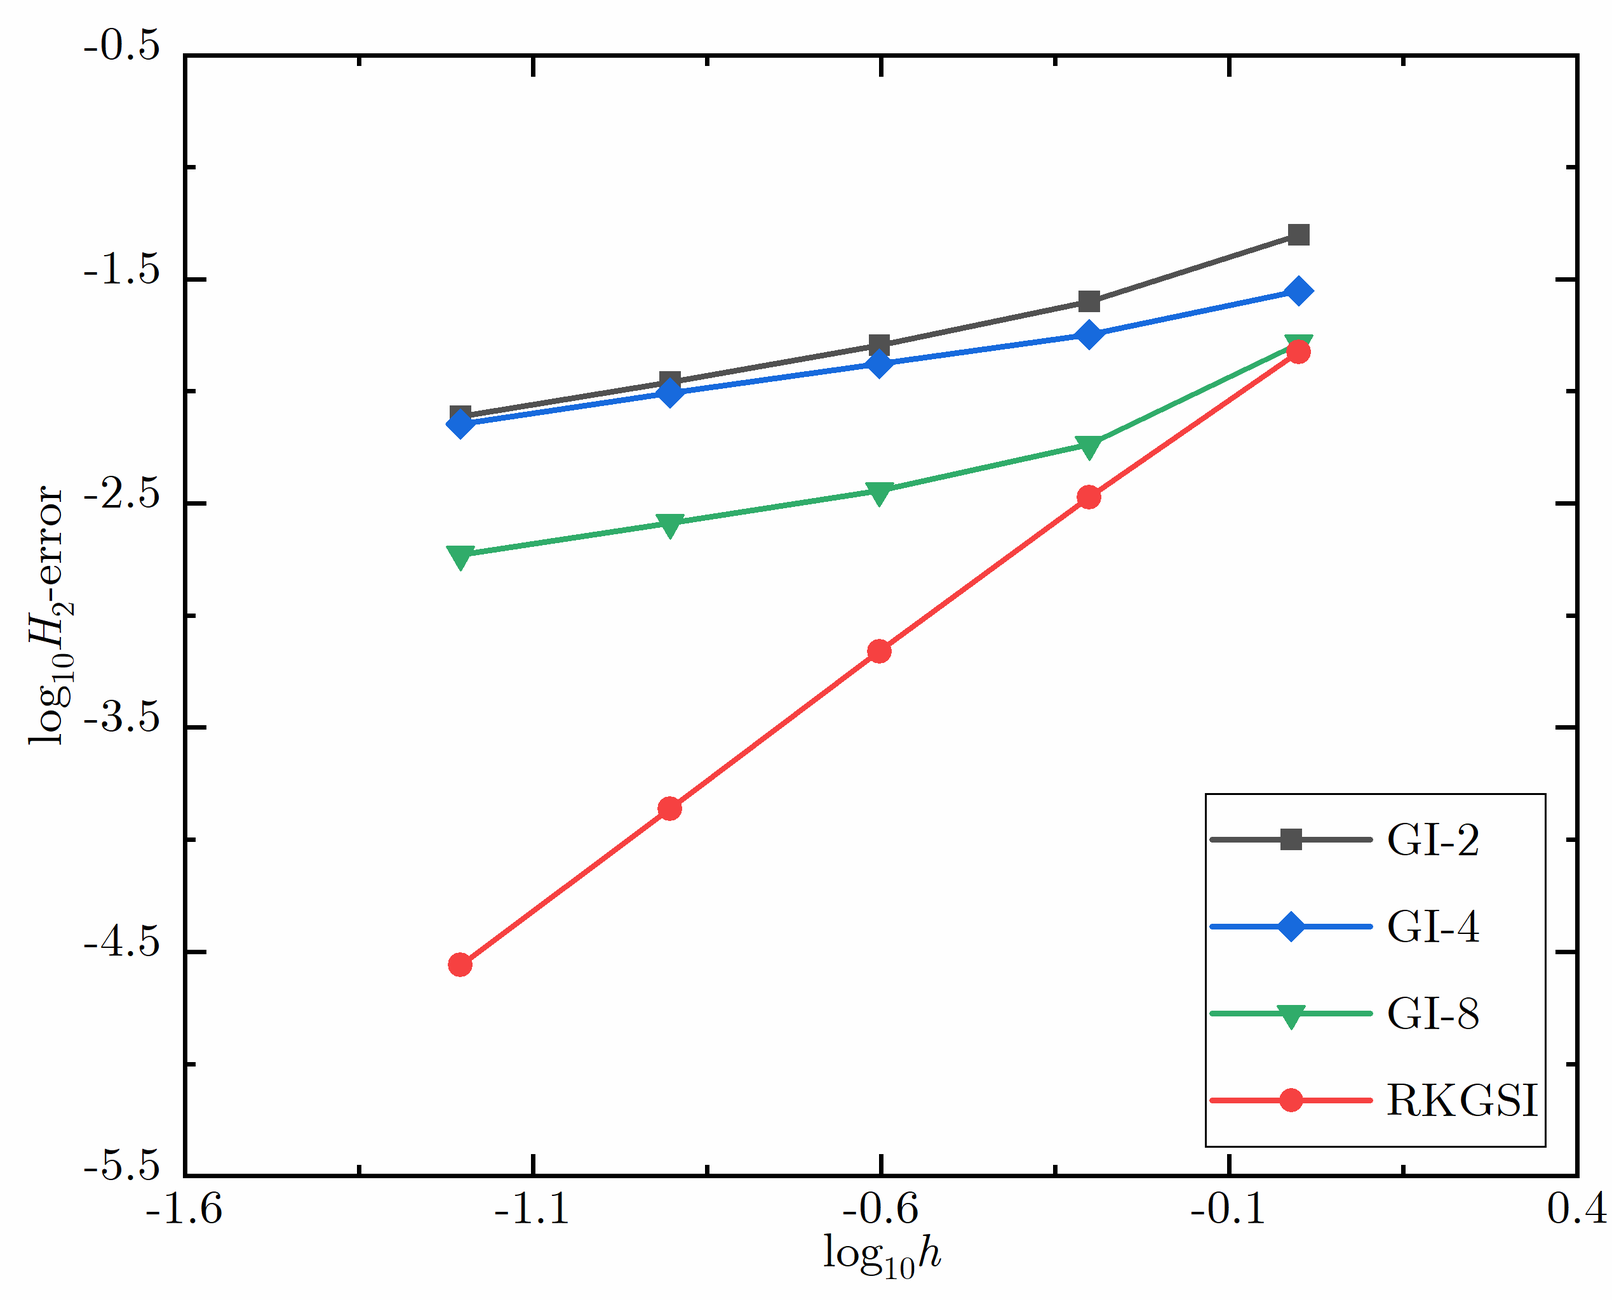
\includegraphics[width=0.55\textwidth]{figs/fig17.png}
\caption{$H_2$-error comparison for the 1D manufactured beam with $p=3$.}\label{fig:17}
\end{figure}

\begin{figure}[pos=htbp]
\centering
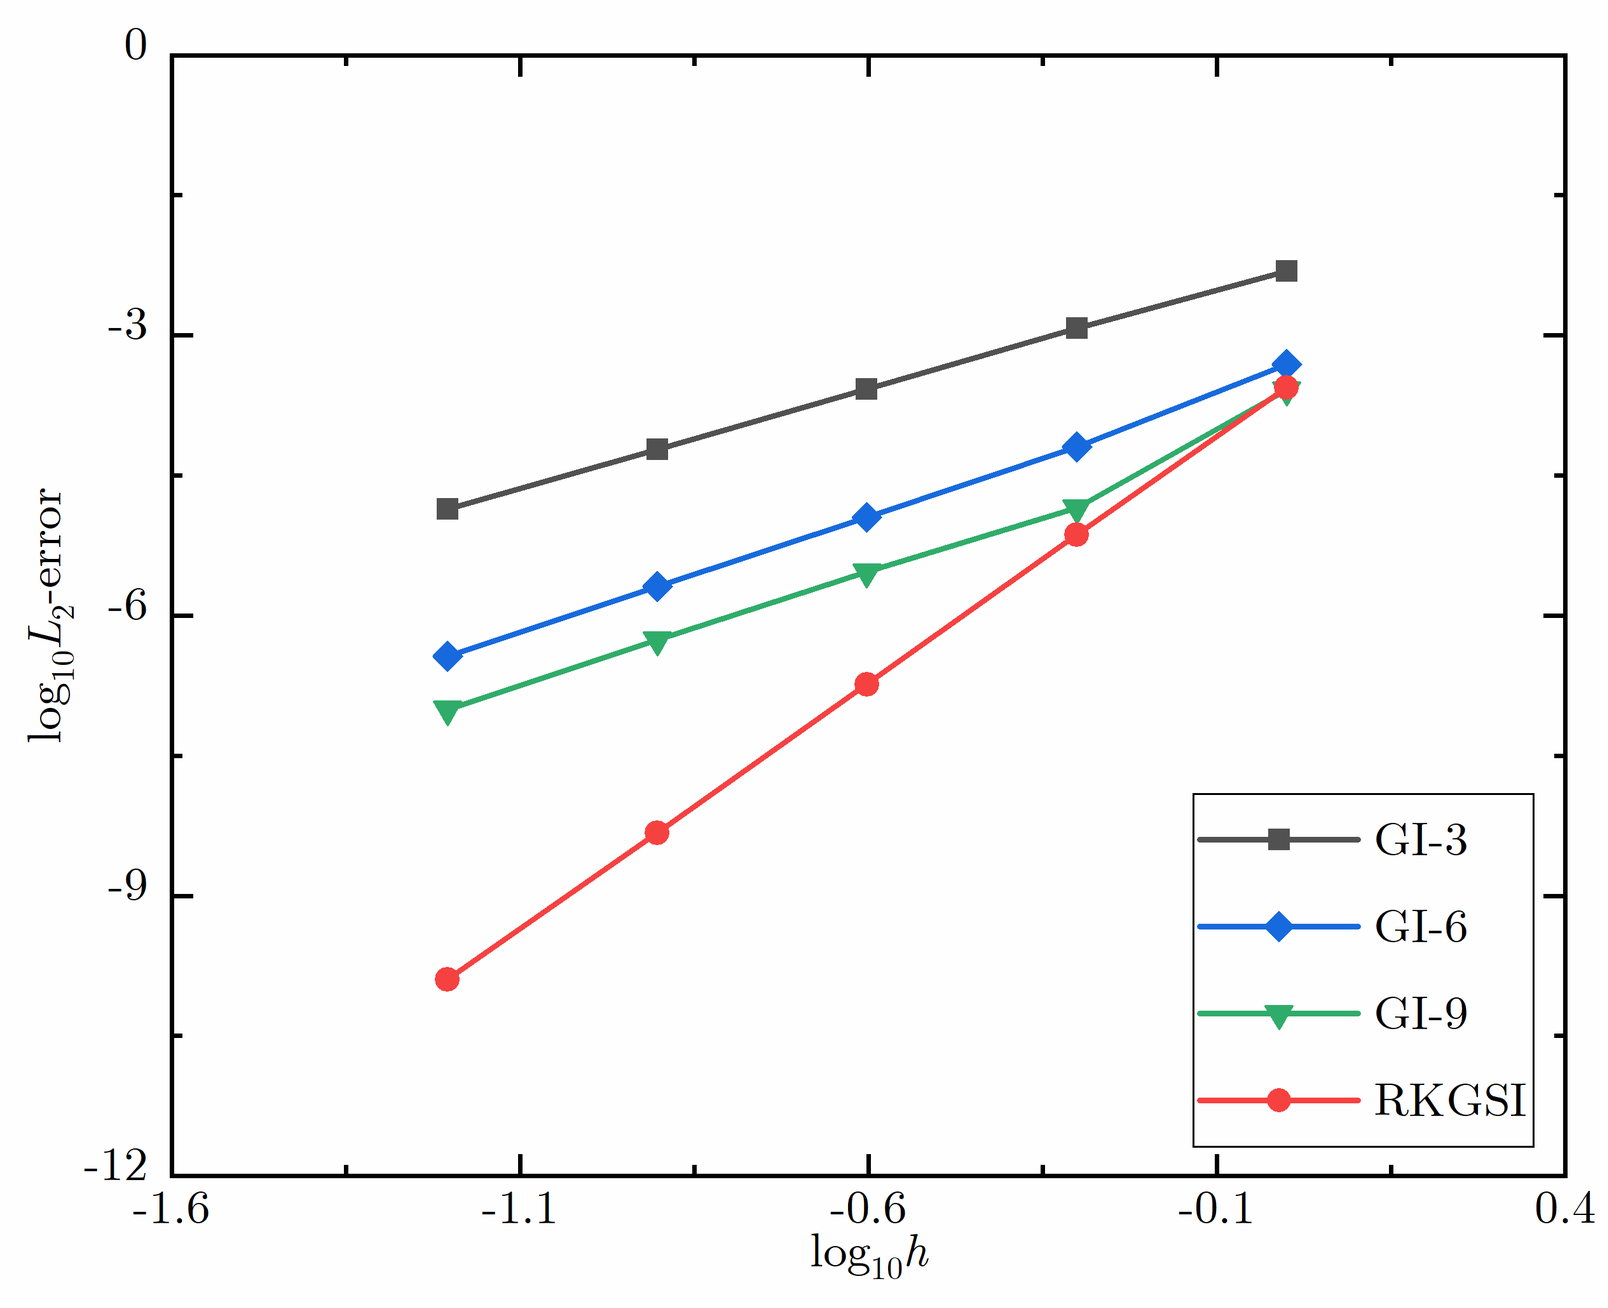
\includegraphics[width=0.55\textwidth]{figs/fig18.png}
\caption{$L_2$-error comparison for the 1D manufactured beam with $p=4$.}\label{fig:18}
\end{figure}

\begin{figure}[pos=htbp]
\centering
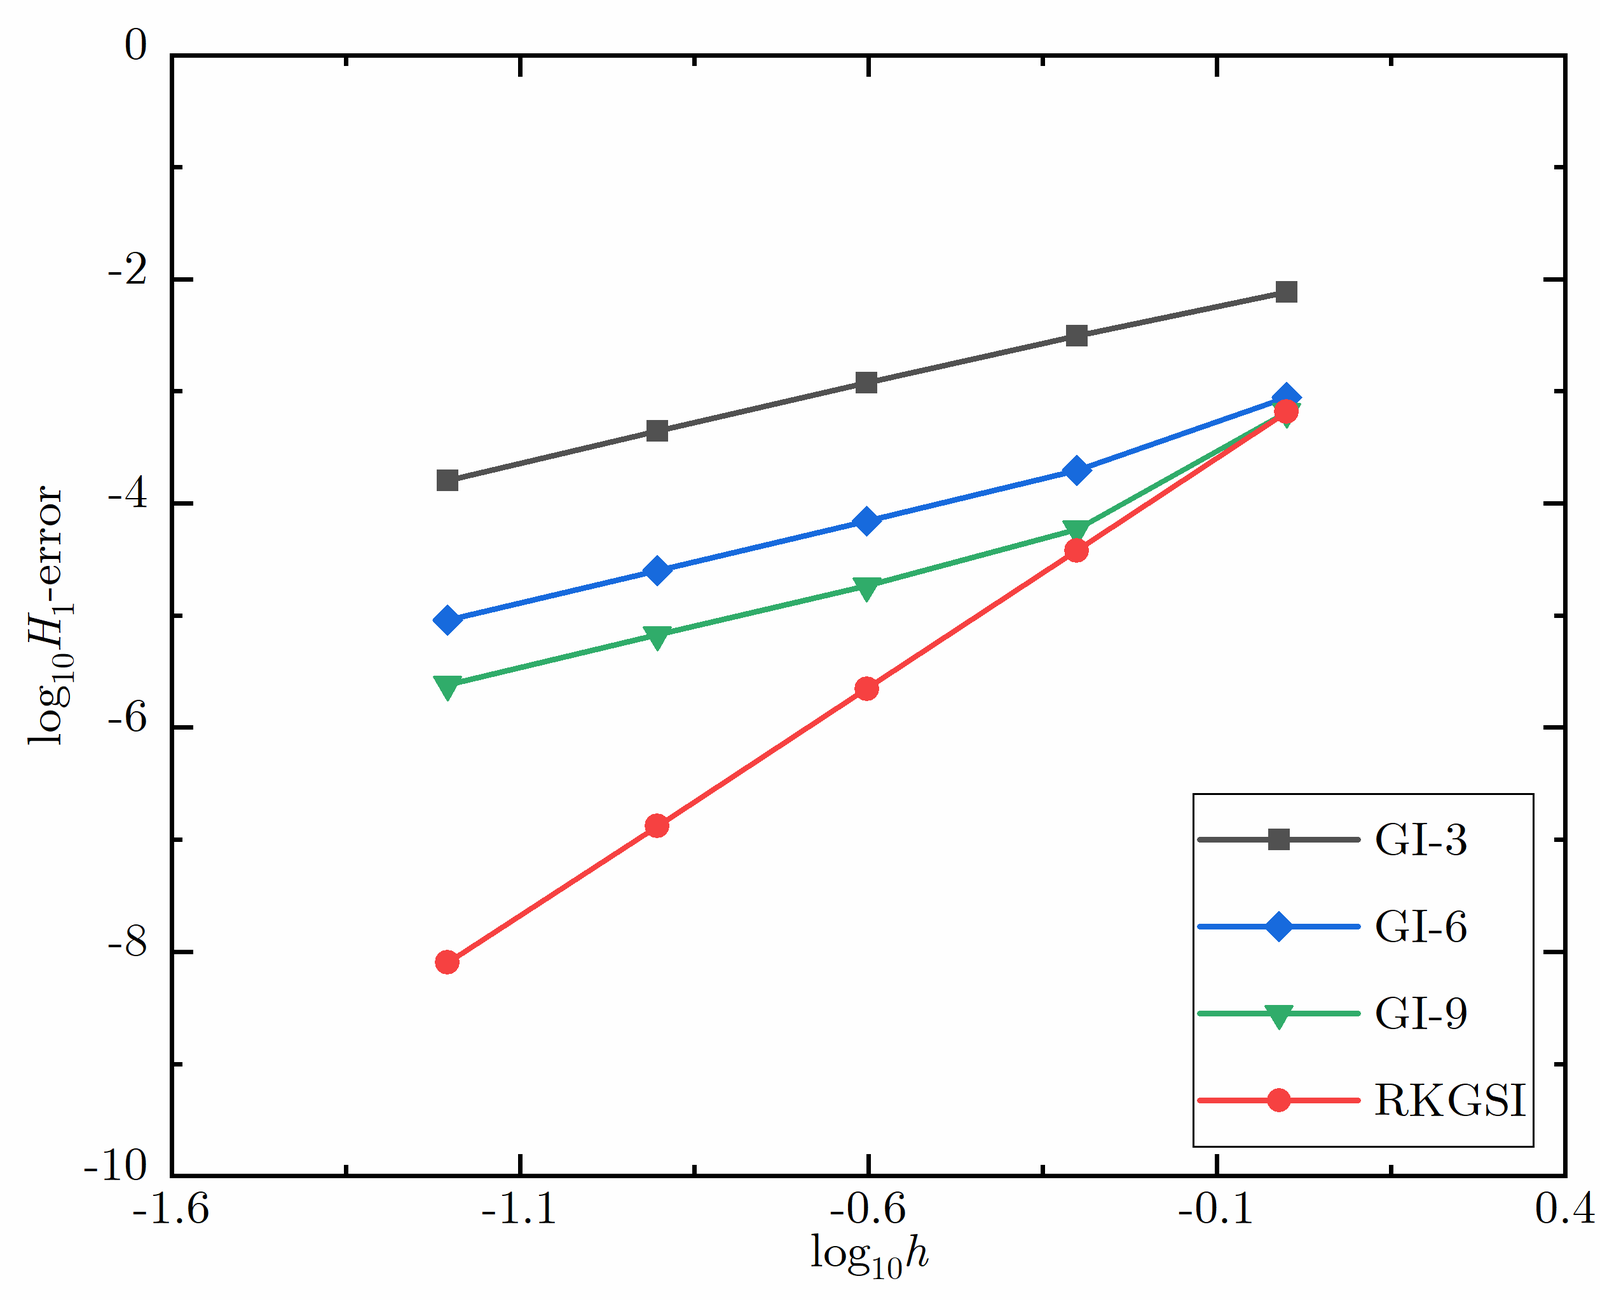
\includegraphics[width=0.55\textwidth]{figs/fig19.png}
\caption{$H_1$-error comparison for the 1D manufactured beam with $p=4$.}\label{fig:19}
\end{figure}

\begin{figure}[pos=htbp]
\centering
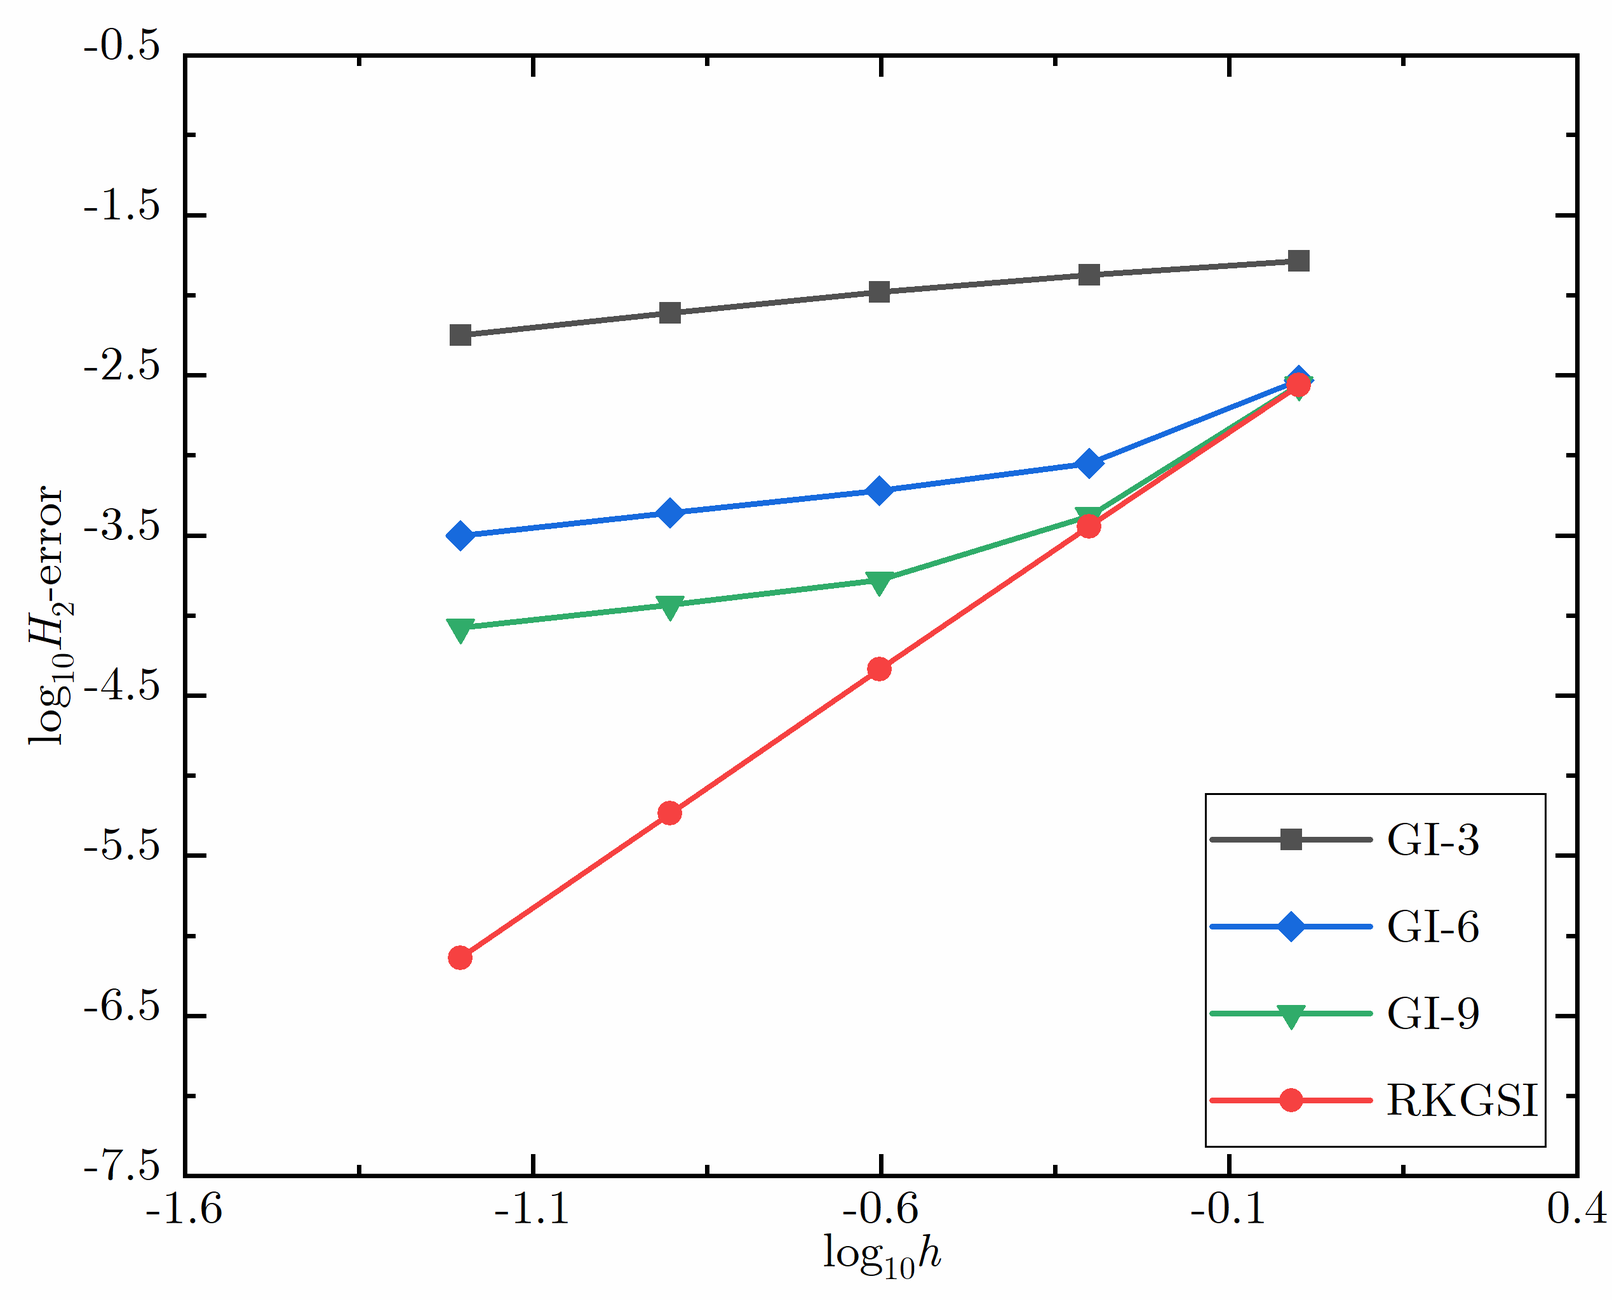
\includegraphics[width=0.55\textwidth]{figs/fig20.png}
\caption{$H_2$-error comparison for the 1D manufactured beam with $p=4$.}\label{fig:20}
\end{figure}

\subsection{2D manufactured plate}\label{sec:manufactured2d}

As shown in Fig. \ref{fig:21}, we perform the assessment of convergence performance on a manufactured plate, whose material and geometric properties are $D=2\times10^{4}$, Poisson's ratio $\nu=0.3$, length $L=10$.
The manufactured solution is state as:
\begin{equation}\label{eq:93}
w=\left(x+2y+1\right)^{8}/1000
\end{equation}

\begin{figure}[pos=htbp]
\centering
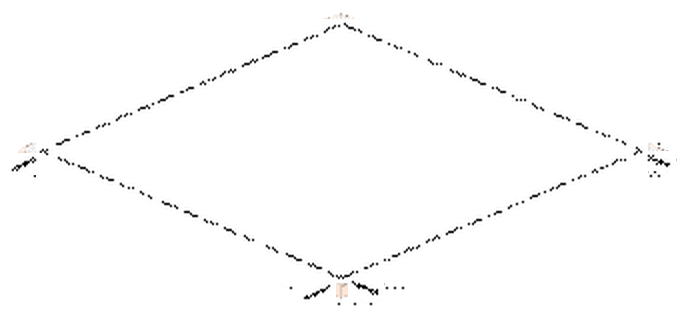
\includegraphics[width=0.6\textwidth]{figs/fig21.png}
\caption{Description of 2D manufactured plate.}\label{fig:21}
\end{figure}

The same as Section \ref{sec:quadratic}, five regular grids with 36, 121, 441, 1681, and 6561 nodes are applied to discrete the 2D domain.
The corresponding results are listed in Figs. \ref{fig:22}--\ref{fig:27}, which clearly evince that, with the reduce of nodal distance, the convergence rates of Gauss integration based method constantly deteriorate until reach the theoretical values, which are far below the optimal ones.
However, no matter which order of basis function is adopted, the convergence rates of RKGSI always keep $(p+1)$, $p$ and $(p-1)$, regarding the $L_2$, $H_1$ and $H_2$ error norms.

\begin{figure}[pos=htbp]
\centering
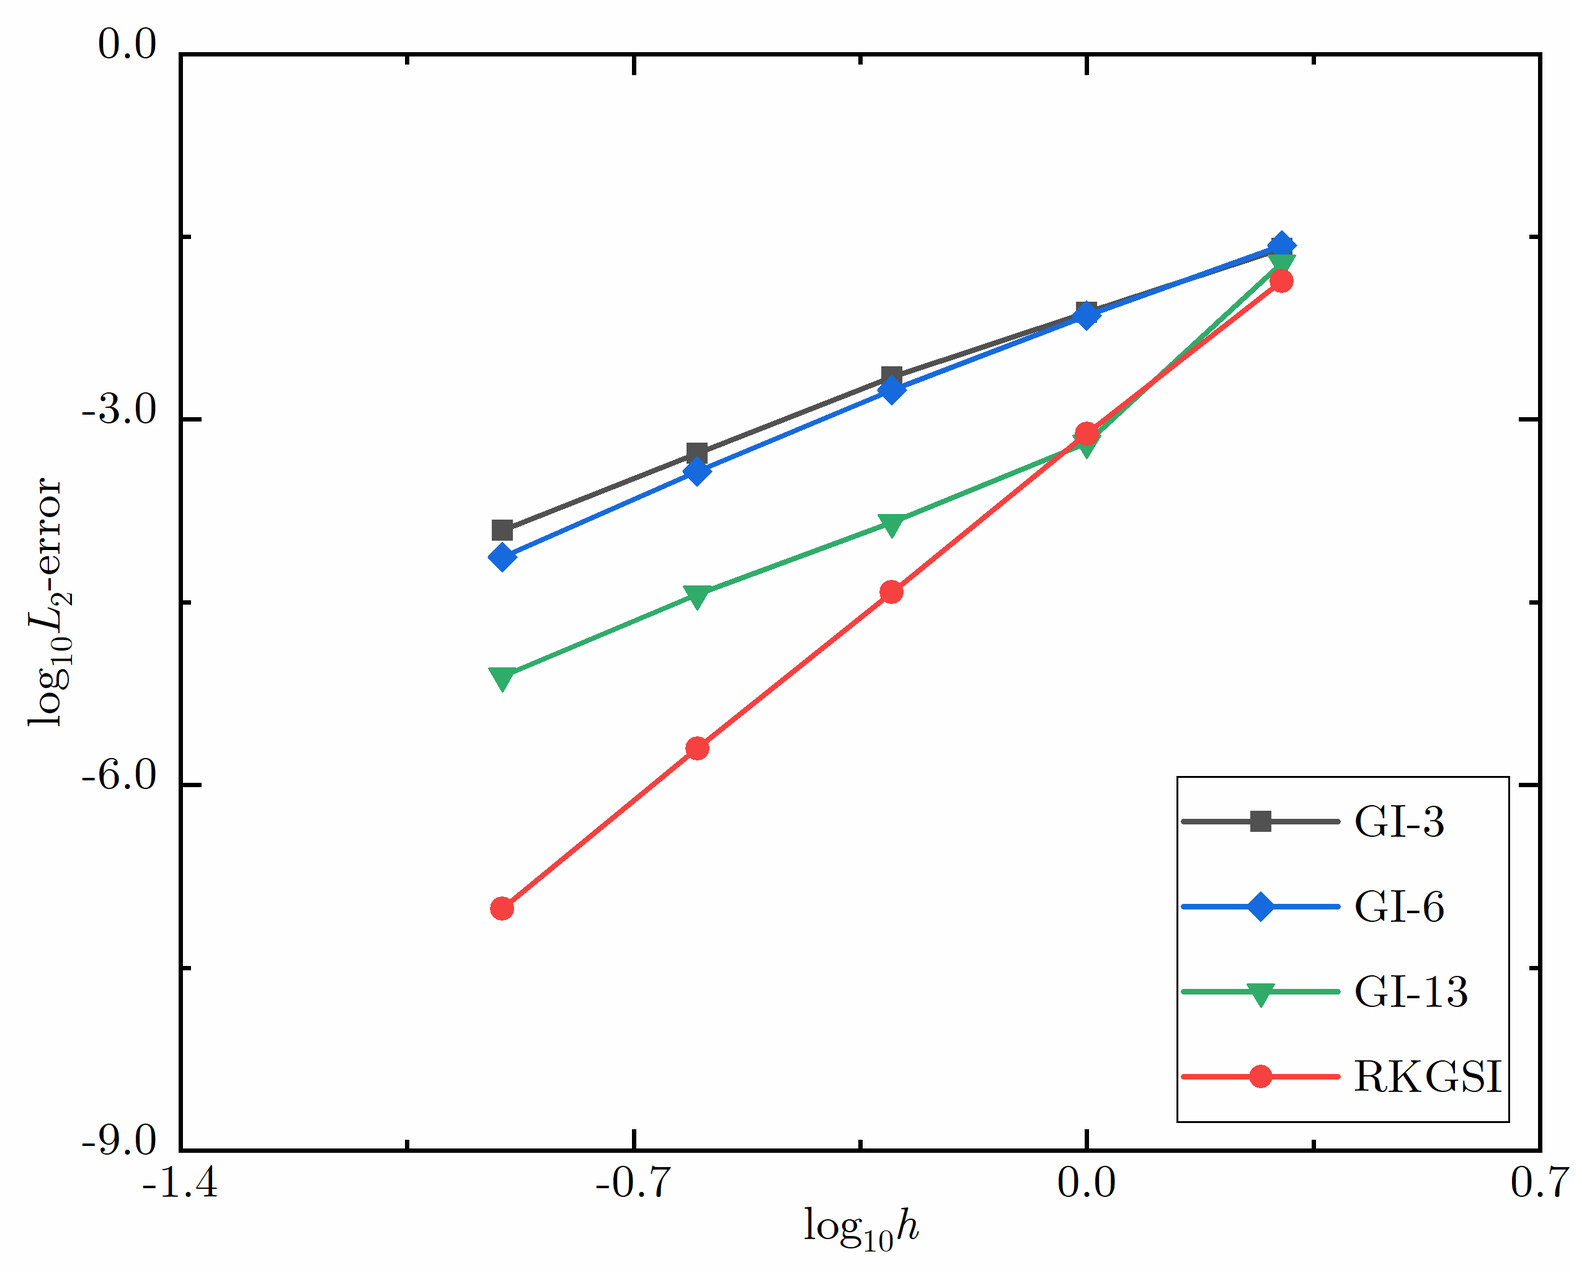
\includegraphics[width=0.55\textwidth]{figs/fig22.png}
\caption{$L_2$-error comparison for the 2D manufactured plate with $p=3$.}\label{fig:22}
\end{figure}

\begin{figure}[pos=htbp]
\centering
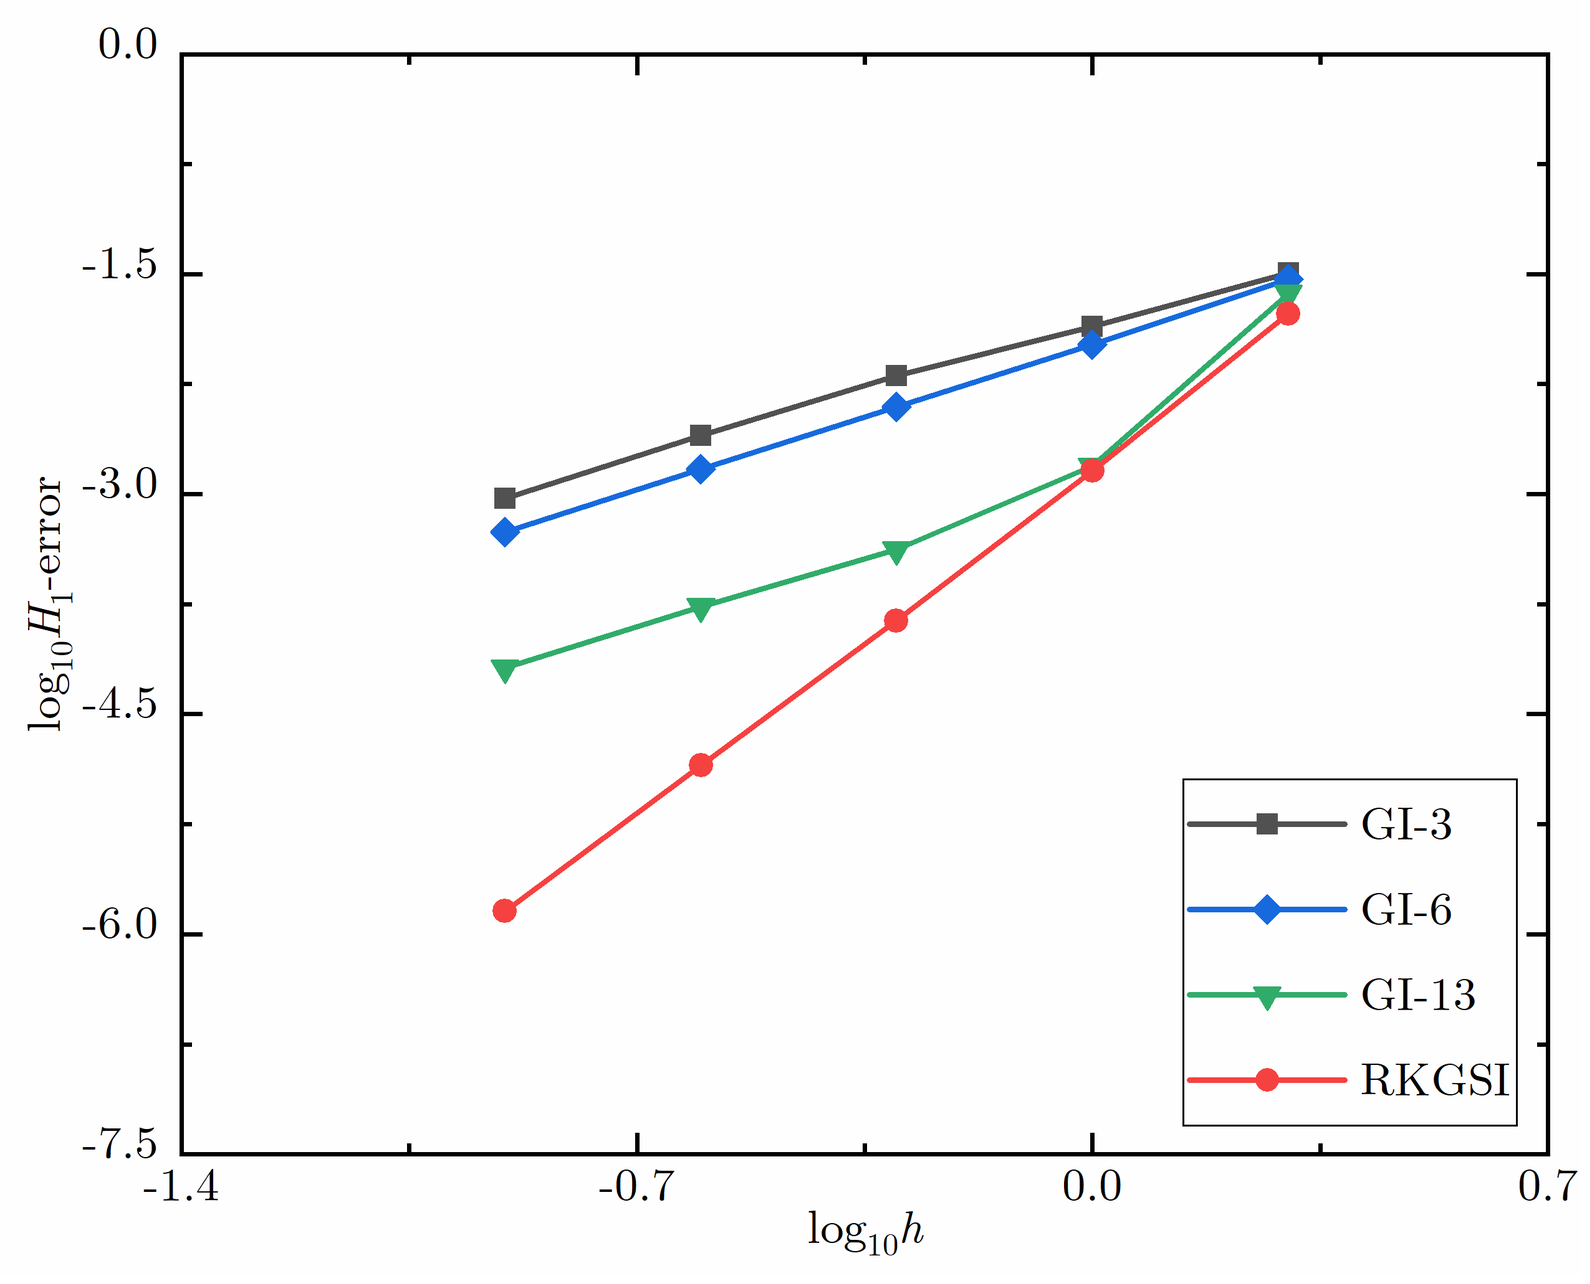
\includegraphics[width=0.55\textwidth]{figs/fig23.png}
\caption{$H_1$-error comparison for the 2D manufactured plate with $p=3$.}\label{fig:23}
\end{figure}

\begin{figure}[pos=htbp]
\centering
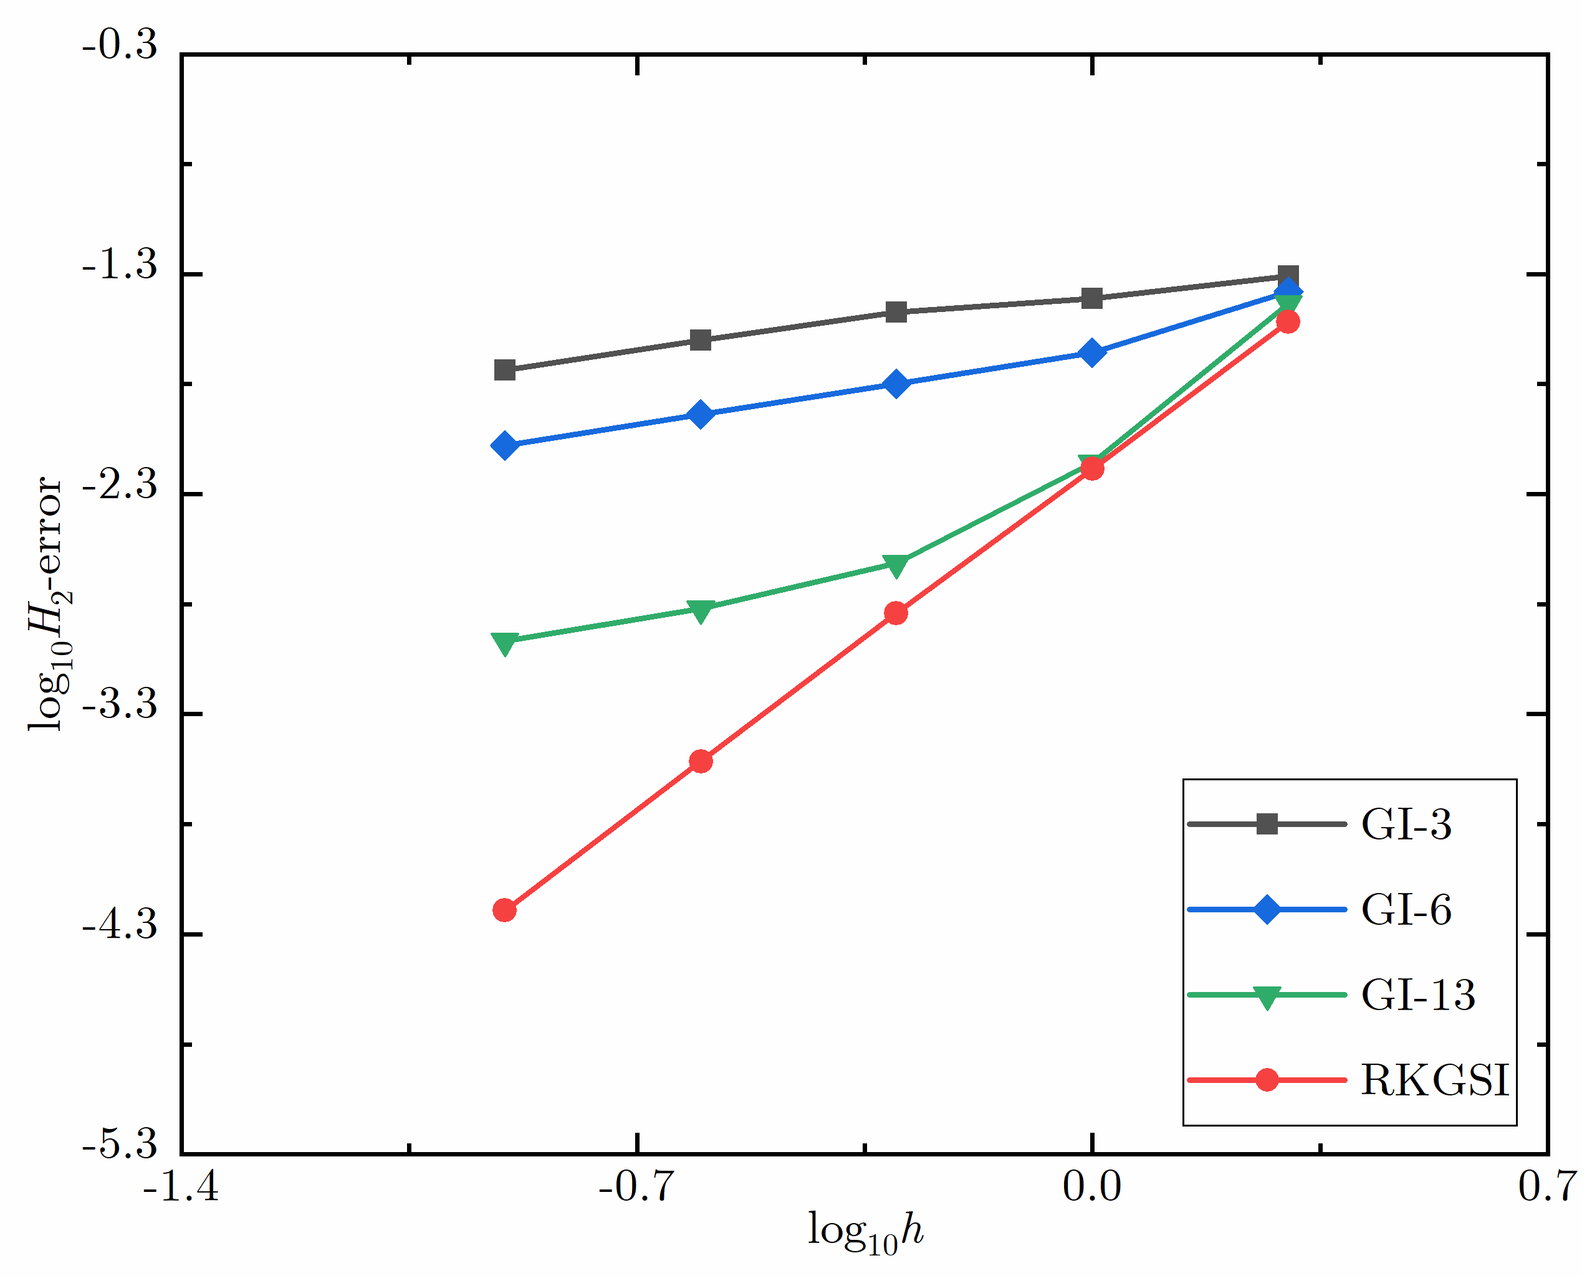
\includegraphics[width=0.55\textwidth]{figs/fig24.png}
\caption{$H_2$-error comparison for the 2D manufactured plate with $p=3$.}\label{fig:24}
\end{figure}

\begin{figure}[pos=htbp]
\centering
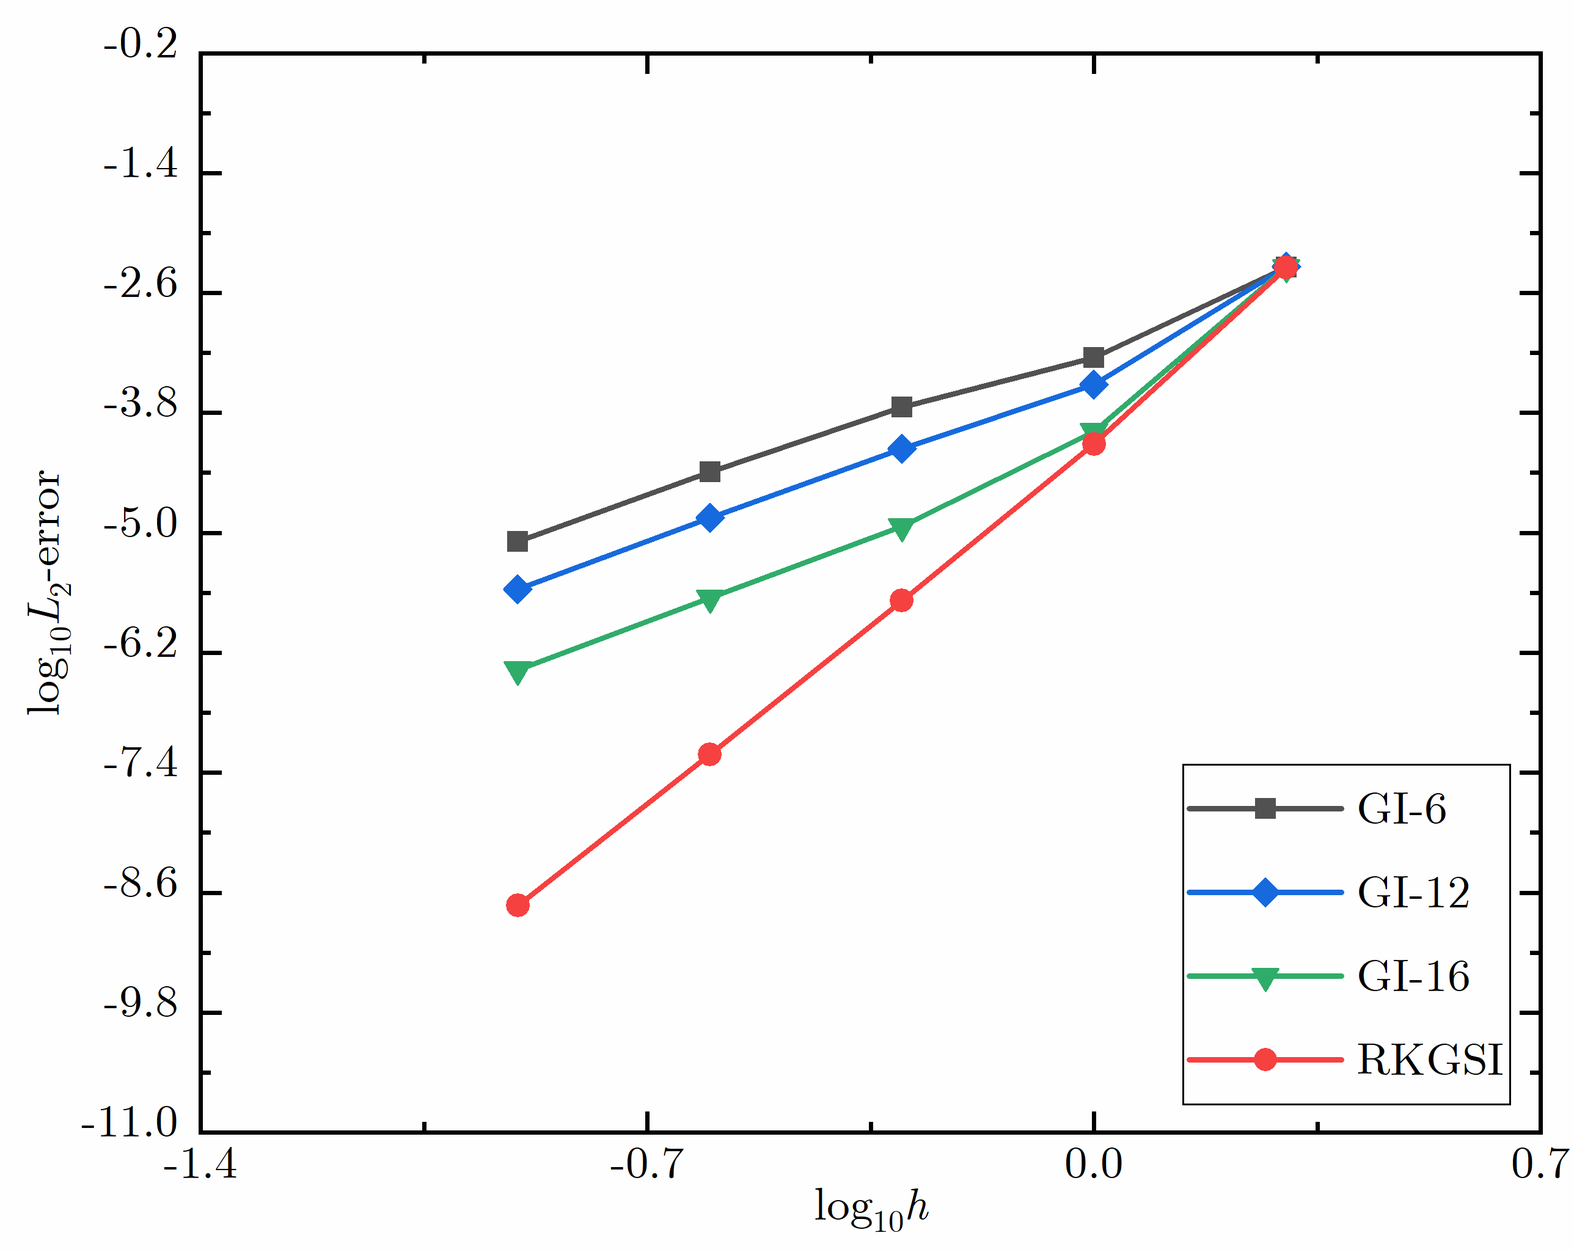
\includegraphics[width=0.55\textwidth]{figs/fig25.png}
\caption{$L_2$-error comparison for the 2D manufactured plate with $p=4$.}\label{fig:25}
\end{figure}

\begin{figure}[pos=htbp]
\centering
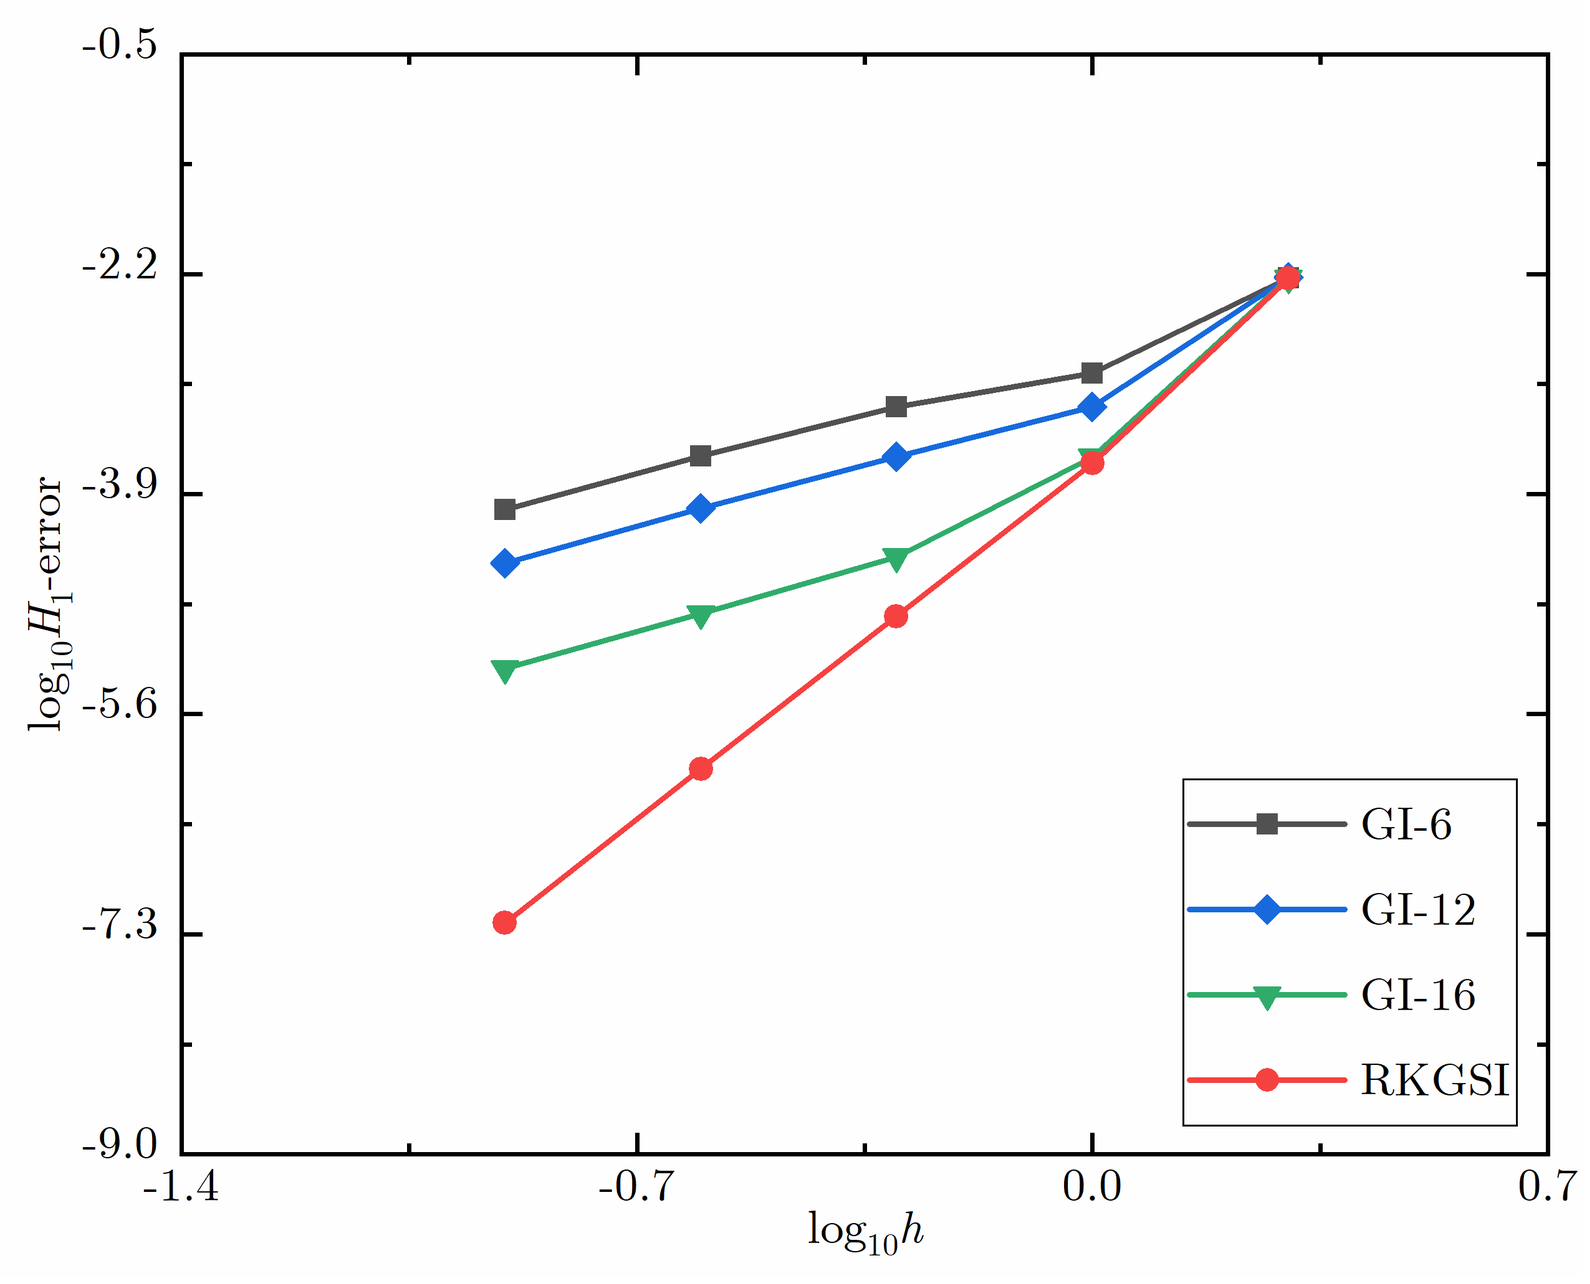
\includegraphics[width=0.55\textwidth]{figs/fig26.png}
\caption{$H_1$-error comparison for the 2D manufactured plate with $p=4$.}\label{fig:26}
\end{figure}

\begin{figure}[pos=htbp]
\centering
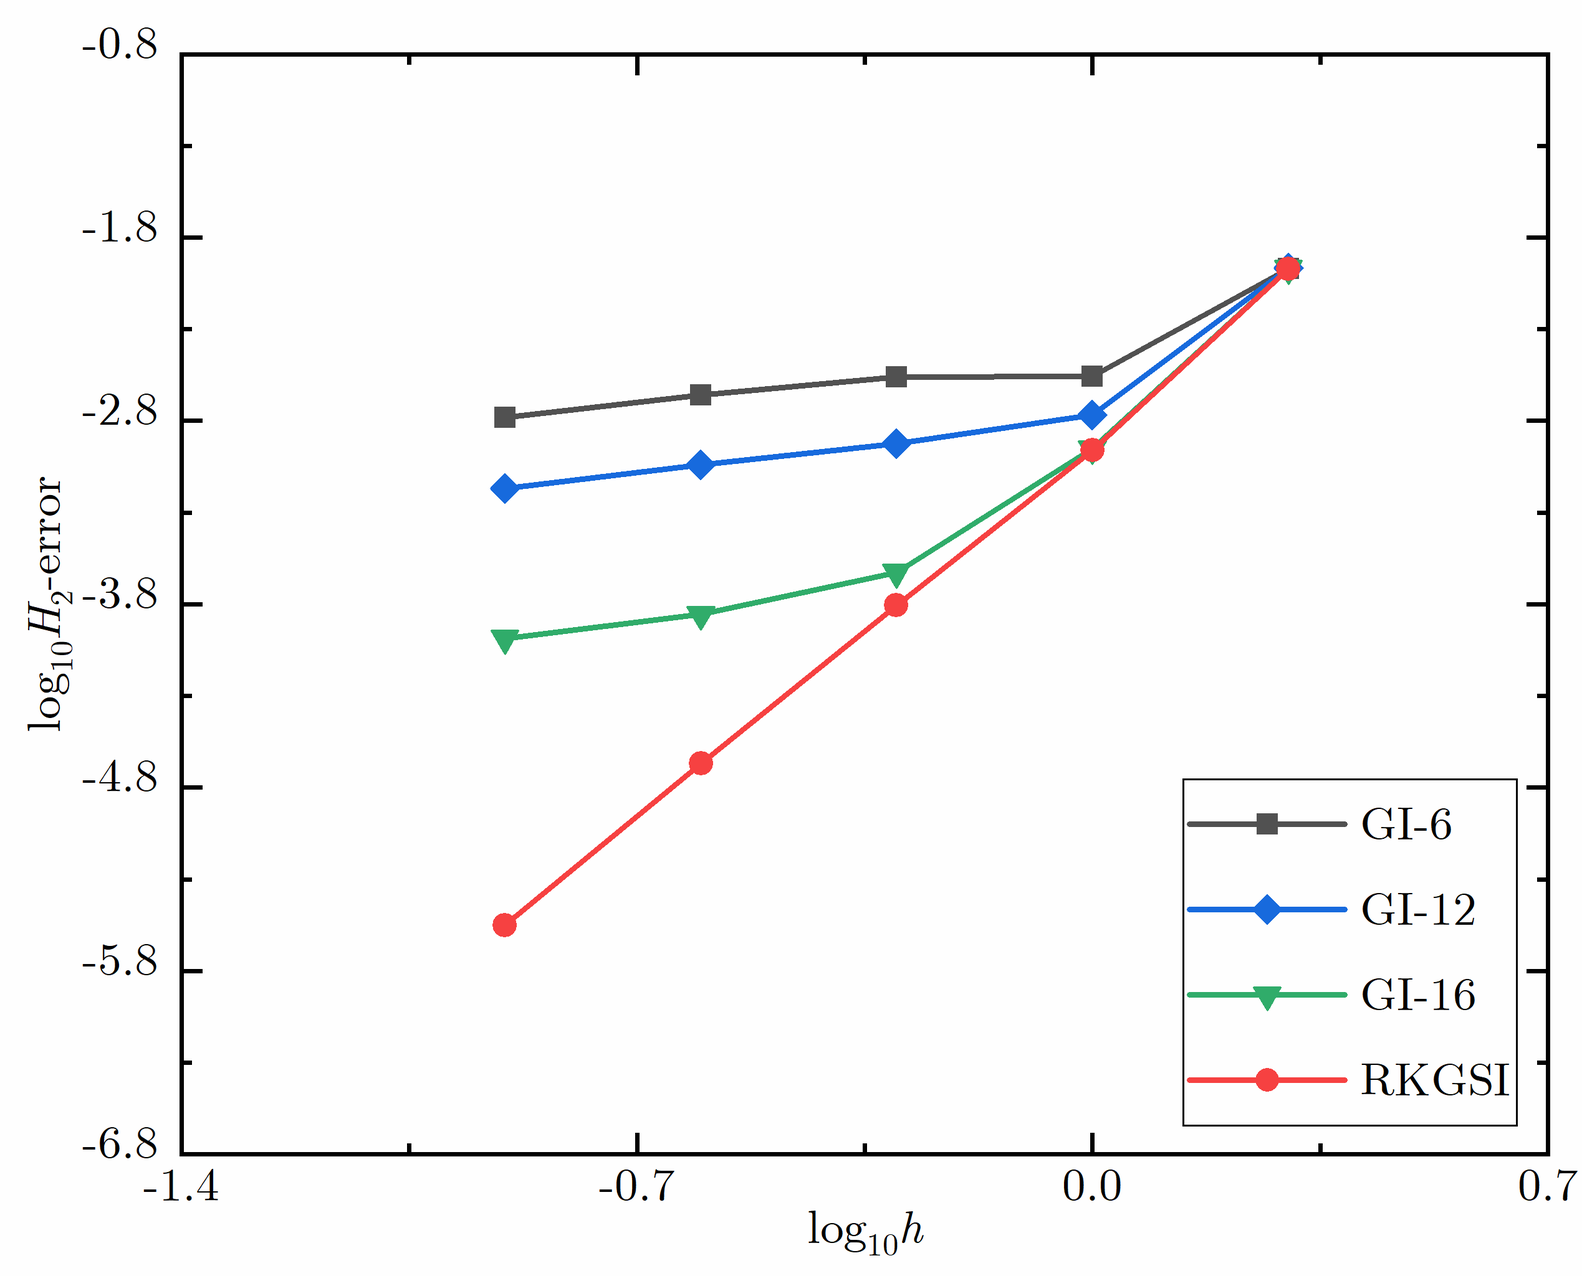
\includegraphics[width=0.55\textwidth]{figs/fig27.png}
\caption{$H_2$-error comparison for the 2D manufactured plate with $p=4$.}\label{fig:27}
\end{figure}

%% ---------------------------------------------------------------------------
%% 5. Conclusions
%% ---------------------------------------------------------------------------
\section{Conclusions}\label{sec:conclusion}

A series of explicit measures for $L_2$, $H_1$ and $H_2$ error estimates of Kirchhoff plate Galerkin meshfree method has been presented in this work, in which the important roles of numerical integration and meshfree approximation on Kirchhoff plate meshfree method were investigated.
It was shown that the integration consistency of meshfree formulation to Kirchhoff plate affects the error estimate of Galerkin orthogonality, thus the convergence rate of overall $L_2$, $H_1$ and $H_2$ errors are mutually controlled by the orders of integration consistency and approximation of meshfree formulation.
More specifically, these error estimates are divided into two parts, in which the first part comes from the error of meshfree interpolation and the second one originates from the order of integration consistency.
Moreover, since the order of meshfree interpolation will constrains the order selection of Lagrange interpolation in $L_2$ error analysis, only a high enough order of meshfree interpolation ($p\ge3$) can ensure $(p+1)$th order of convergence rate for $L_2$ error, otherwise, only $p$th order of convergence rate could be achieved even with the premise of enough order of the integration consistency.
In conclusion, since traditional numerical integration methods will cause the loss of orthogonality due to the poor integration consistency, thus cannot realize optimal convergence performance even with increased integral points.
Also, the convergence rate of $L_2$ error for quadratic meshfree formulation to Kirchhoff plate is limited to $p$th order.
Thus with the expectation of $(p+1)$th order convergence performance, cubic and quartic meshfree formulations are more suitable for Kirchhoff plate analysis.
A list of numerical examples well proves the proposed conclusions for error estimates of Kirchhoff plate meshfree methods.


%% ---------------------------------------------------------------------------
%% Bibliography
%% ---------------------------------------------------------------------------
%% ---------------------------------------------------------------------------
%% References -- numeric, in citation order (as numbered in the source)
%% ---------------------------------------------------------------------------
\begin{thebibliography}{51}

\bibitem{ref1} Belytschko T, Krongauz Y, Organ D, Fleming M, Krysl P (1996) Meshless methods: an overview and recent developments. \emph{Computer Methods in Applied Mechanics and Engineering} 139: 3--47.

\bibitem{ref2} Li S, Liu W K (2004) \emph{Meshfree Particle Methods}. Springer-Verlag.

\bibitem{ref3} Zhang X, Liu Y (2004) \emph{Meshless Methods}. Tsinghua University Press and Springer-Verlag.

\bibitem{ref4} Liu G R (2009) \emph{Meshfree Methods: Moving beyond the Finite Element Method}. 2nd ed. CRC Press.

\bibitem{ref5} Chen J S, Hillman M, Chi S W (2017) Meshfree methods: progress made after 20 years. \emph{Journal of Engineering Mechanics-ASCE} 143: 04017001.

\bibitem{ref6} Wang D, Wang J, Wu J (2020) Arbitrary order recursive formulation of meshfree gradients with application to superconvergent collocation analysis of {Kirchhoff} plates. \emph{Computational Mechanics} 65: 877--903.

\bibitem{ref7} Hillman M, Lin K C (2021) Nodally integrated thermo-mechanical {RKPM}: {Part I} -- Thermoelasticity. \emph{Computational Mechanics} 68: 795--820.

\bibitem{ref8} Zienkiewicz O C, Taylor R L, Fox D (2014) \emph{The Finite Element Method for Solid and Structural Mechanics}. 7th ed. Elsevier.

\bibitem{ref9} Belytschko T, Lu Y Y, Gu L (1994) Element-free {Galerkin} methods. \emph{International Journal for Numerical Methods in Engineering} 37: 229--256.

\bibitem{ref10} Belytschko T, Lu Y Y, Gu L, Tabbara M (1995) Element-free {Galerkin} methods for static and dynamic fracture. \emph{International Journal of Solids and Structures} 32: 2547--2570.

\bibitem{ref11} Liu W K, Han W, Lu H, Li S, Cao J (2004) Reproducing kernel element method. {Part I}: Theoretical formulation. \emph{Computer Methods in Applied Mechanics and Engineering} 193: 933--951.

\bibitem{ref12} Arroyo M, Ortiz M (2006) Local maximum-entropy approximation schemes: a seamless bridge between finite elements and meshfree methods. \emph{International Journal for Numerical Methods in Engineering} 65: 2167--2202.

\bibitem{ref13} Liu G R, Dai K Y, Nguyen T T (2007) A smoothed finite element method for mechanics problems. \emph{Computational Mechanics} 39: 859--877.

\bibitem{ref14} Duarte C A, Oden J T (1996) An hp adaptive method using clouds. \emph{Computer Methods in Applied Mechanics and Engineering} 139: 237--262.

\bibitem{ref15} Sukumar N, Moran B, Belytschko T (1998) The natural element method in solid mechanics. \emph{International Journal for Numerical Methods in Engineering} 43: 839--887.

\bibitem{ref16} Wang J G, Liu G R (2002) A point interpolation meshless method based on radial basis functions. \emph{International Journal for Numerical Methods in Engineering} 54: 1623--1648.

\bibitem{ref17} Guan P C, Chi S W, Chen J S, Slawson T R, Roth M J (2011) Semi-{Lagrangian} reproducing kernel particle method for fragment-impact problems. \emph{International Journal of Impact Engineering} 38: 1033--1047.

\bibitem{ref18} Wang D, Chen P (2014) Quasi-convex reproducing kernel meshfree method. \emph{Computational Mechanics} 54: 689--709.

\bibitem{ref19} Metsis P, Lantzounis N, Papadrakakis M (2015) A new hierarchical partition of unity formulation of {EFG} meshless methods. \emph{Computer Methods in Applied Mechanics and Engineering} 283: 782--805.

\bibitem{ref20} Trask N, Bochev P, Perego M (2020) A conservative, consistent, and scalable meshfree mimetic method. \emph{Journal of Computational Physics} 409: 109187.

\bibitem{ref21} Krysl P, Belytschko T (1995) Analysis of thin plates by the element-free {Galerkin} method. \emph{Computational Mechanics} 17(1--2): 26--35.

\bibitem{ref22} Liu G R, Chen X L (2001) A mesh-free method for static and free vibration analyses of thin plates of complicated shape. \emph{Journal of Sound and Vibration} 241: 839--855.

\bibitem{ref23} Liu L, Liu G R, Tan V B C (2002) Element free method for static and free vibration analysis of spatial thin shell structures. \emph{Computer Methods in Applied Mechanics and Engineering} 191: 5923--5942.

\bibitem{ref24} Gu Y T, Liu G R (2001) A meshless local {Petrov--Galerkin} ({MLPG}) formulation for static and free vibration analyses of thin plates. \emph{Computer Modeling in Engineering and Sciences} 2: 463--476.

\bibitem{ref25} Simkins D C, Li S, Lu H, Liu W K (2004) Reproducing kernel element method. {Part IV}: Globally compatible triangular hierarchy. \emph{Computer Methods in Applied Mechanics and Engineering} 193: 1013--1034.

\bibitem{ref26} Wang D, Chen J S (2008) A {Hermite} reproducing kernel approximation for thin-plate analysis with sub-domain stabilized conforming integration. \emph{International Journal for Numerical Methods in Engineering} 74: 368--390.

\bibitem{ref27} Oh H-S, Davis C, Jeong J W (2012) Meshfree particle methods for thin plates. \emph{Computer Methods in Applied Mechanics and Engineering} 209--212: 156--171. \url{https://doi.org/10.1016/j.cma.2011.10.011}

\bibitem{ref28} Deng L, Wang D, Wang J, Wu J (2019) A gradient smoothing {Galerkin} meshfree method for thin plate analysis with linear basis function. \emph{Chinese Journal of Theoretical and Applied Mechanics} 51(3): 690--702.

\bibitem{ref29} Dolbow J, Belytschko T (1999) Numerical integration of the {Galerkin} weak form in meshfree methods. \emph{Computational Mechanics} 23: 219--230.

\bibitem{ref30} Babu{\v{s}}ka I, Banerjee U, Osborn J E, Li Q L (2008) Quadrature for meshless methods. \emph{International Journal for Numerical Methods in Engineering} 76: 1434--1470.

\bibitem{ref31} Chen J S, Wu C T, Yoon S, You Y (2001) A stabilized conforming nodal integration for {Galerkin} meshfree methods. \emph{International Journal for Numerical Methods in Engineering} 50: 435--466.

\bibitem{ref32} Chen J S, Yoon S, Wu C T (2002) Nonlinear version of stabilized conforming nodal integration for {Galerkin} meshfree methods. \emph{International Journal for Numerical Methods in Engineering} 53: 2587--2615.

\bibitem{ref33} Wang D, Chen J S (2004) Locking-free stabilized conforming nodal integration for meshfree {Mindlin--Reissner} plate formulation. \emph{Computer Methods in Applied Mechanics and Engineering} 193: 1065--1083.

\bibitem{ref34} Chen J S, Wang D (2006) A constrained reproducing kernel particle formulation for shear deformable shell in {Cartesian} coordinates. \emph{International Journal for Numerical Methods in Engineering} 68: 151--172.

\bibitem{ref35} Duan Q, Li X, Zhang H, Belytschko T (2012) Second-order accurate derivatives and integration schemes for meshfree methods. \emph{International Journal for Numerical Methods in Engineering} 92: 399--424.

\bibitem{ref36} Wang D, Chen J S (2008) A {Hermite} reproducing kernel approximation for thin-plate analysis with sub-domain stabilized conforming integration. \emph{International Journal for Numerical Methods in Engineering} 74: 368--390.

\bibitem{ref37} Wang D, Wu Y (2008) An efficient {Galerkin} meshfree analysis of shear deformable cylindrical panels. \emph{Interaction and Multiscale Mechanics} 1: 339--355.

\bibitem{ref38} Wang D, Lin Z (2011) Dispersion and transient analyses of {Hermite} reproducing kernel {Galerkin} meshfree method with sub-domain stabilized conforming integration for thin beam and plate structures. \emph{Computational Mechanics} 48: 47--63.

\bibitem{ref39} Wang D, Song C, Peng H (2015) A circumferentially enhanced {Hermite} reproducing kernel meshfree method for buckling analysis of {Kirchhoff--Love} cylindrical shells. \emph{International Journal of Structural Stability and Dynamics} 15: 1450090.

\bibitem{ref40} Duan Q, Gao X, Wang B, Li X, Zhang H, Belytschko T, Shao Y (2014) Consistent element-free {Galerkin} method. \emph{International Journal for Numerical Methods in Engineering} 99: 79--101.

\bibitem{ref41} Chen J S, Hillman M, R{\"u}ter M (2013) An arbitrary order variationally consistent integration for {Galerkin} meshfree methods. \emph{International Journal for Numerical Methods in Engineering} 95: 387--418.

\bibitem{ref42} Wang D, Wu J (2016) An efficient nesting sub-domain gradient smoothing integration algorithm with quadratic exactness for {Galerkin} meshfree methods. \emph{Computer Methods in Applied Mechanics and Engineering} 298: 485--519.

\bibitem{ref43} Wang D, Wu J (2019) An inherently consistent reproducing kernel gradient smoothing framework toward efficient {Galerkin} meshfree formulation with explicit quadrature. \emph{Computer Methods in Applied Mechanics and Engineering} 349: 628--672.

\bibitem{ref44} Wu J, Wang D, Lin Z, Qi D (2020) An efficient gradient smoothing meshfree formulation for the fourth-order phase field modeling of brittle fracture. \emph{Computational Particle Mechanics} 7: 193--207.

\bibitem{ref45} Du H, Wu J, Wang D, et al. (2022) A unified reproducing kernel gradient smoothing {Galerkin} meshfree approach to strain gradient elasticity. \emph{Computational Mechanics} 70: 73--100.

\bibitem{ref46} Liu W K, Li S, Belytschko T (1997) Moving least-square reproducing kernel methods ({I}) {Methodology} and convergence. \emph{Computer Methods in Applied Mechanics and Engineering} 143: 113--154.

\bibitem{ref47} Salehi R, Dehghan M (2013) A moving least square reproducing polynomial meshless method. \emph{Applied Numerical Mathematics} 69: 34--58.

\bibitem{ref48} Han W, Meng X (2001) Error analysis of the reproducing kernel particle method. \emph{Computer Methods in Applied Mechanics and Engineering} 190: 6157--6181.

\bibitem{ref49} Osorio M, French D (2013) Error estimates for a multidimensional meshfree {Galerkin} method with diffuse derivatives and stabilization. \emph{Ingenier{\'i}a y Ciencia} 9: 53--76.

\bibitem{ref50} Wu J, Wang D (2021) An accuracy analysis of {Galerkin} meshfree methods accounting for numerical integration. \emph{Computer Methods in Applied Mechanics and Engineering} 375: 113631.

\bibitem{ref51} Quarteroni A, Valli A (1994) \emph{Numerical Approximation of Partial Differential Equations}. Springer.

\end{thebibliography}


\end{document}
